\section{DOM fit of \oSix}
\label{o16DOMOutput}
\begin{figure}[hbtp]
    \captionsetup[subfigure]{labelformat=empty}
    \centering
    \begin{subfigure}[c]{0.39\textheight}
        \centering
        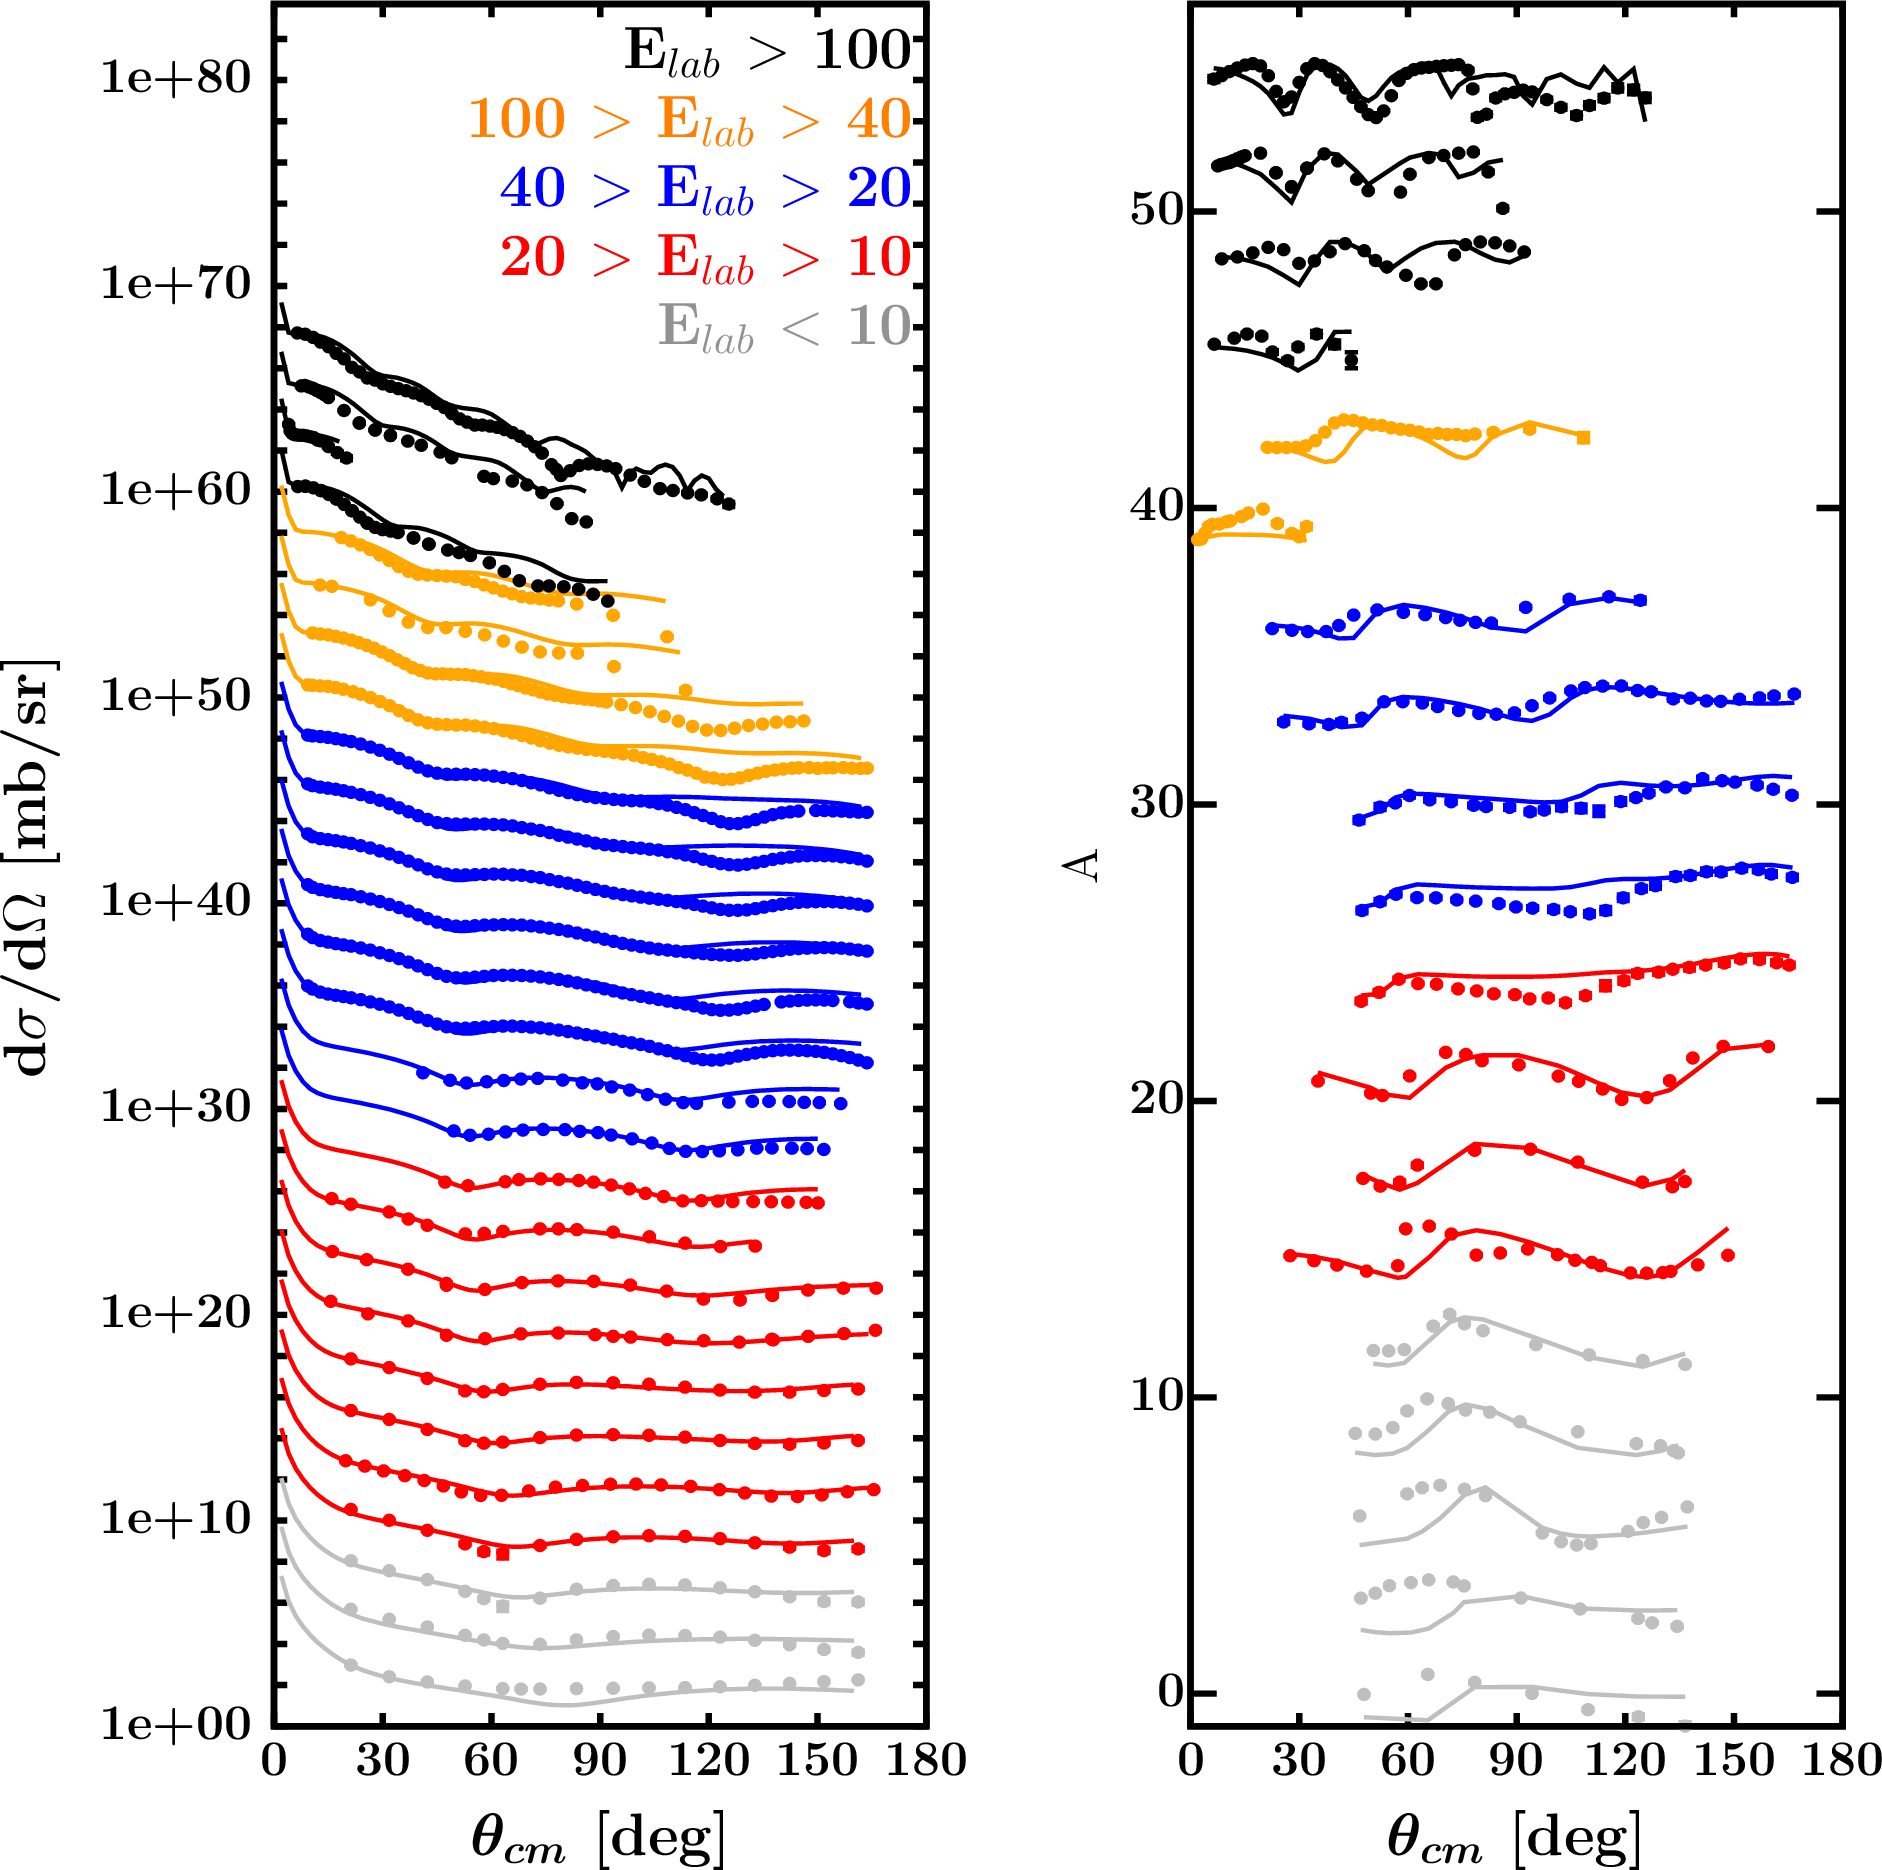
\includegraphics[width=\linewidth]{figures/o16_protonElastic.png}
        \caption{\oSix\ proton elastic scattering}
        \label{DOMFitData_o16_proton_elastic}
    \end{subfigure}\hspace{6pt}
    \begin{subfigure}[c]{0.39\textheight}
        \centering
        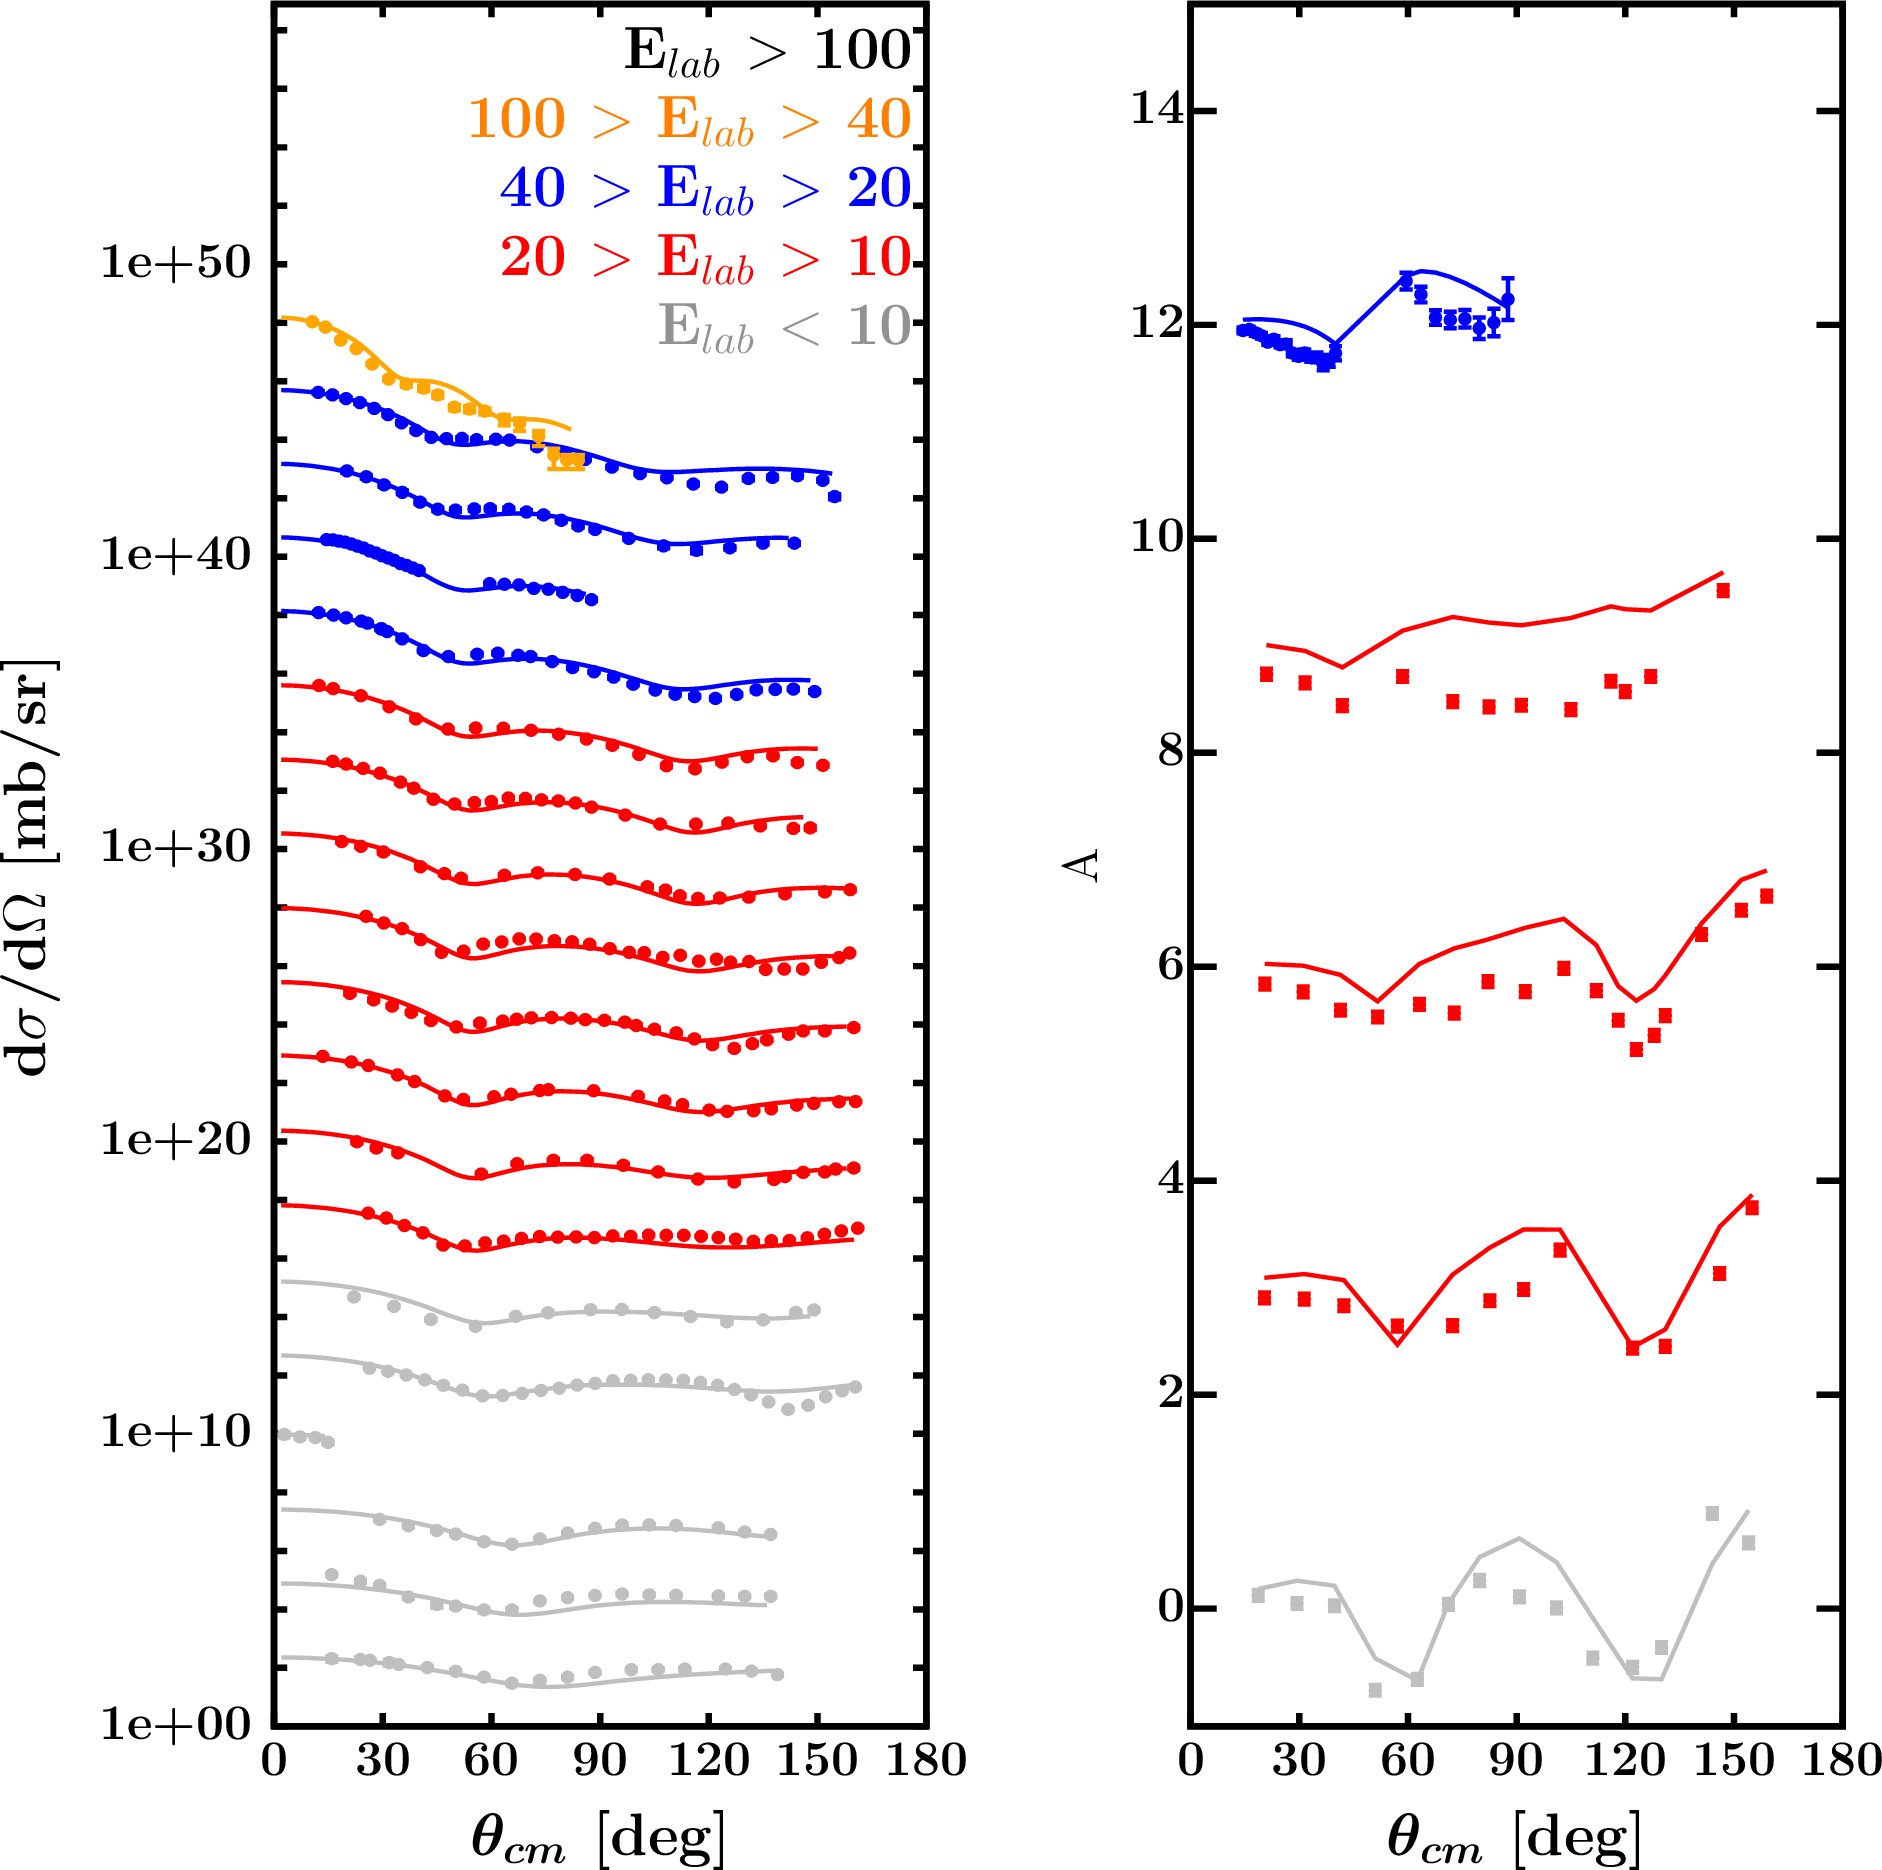
\includegraphics[width=0.52\linewidth]{figures/o16_neutronElastic.png}
        \caption{\oSix\ neutron elastic scattering}
        \label{DOMFitData_o16_neutron_elastic}
    \end{subfigure}\vspace{0.70in}
    \begin{subfigure}[c]{0.45\textwidth}
        \centering
        %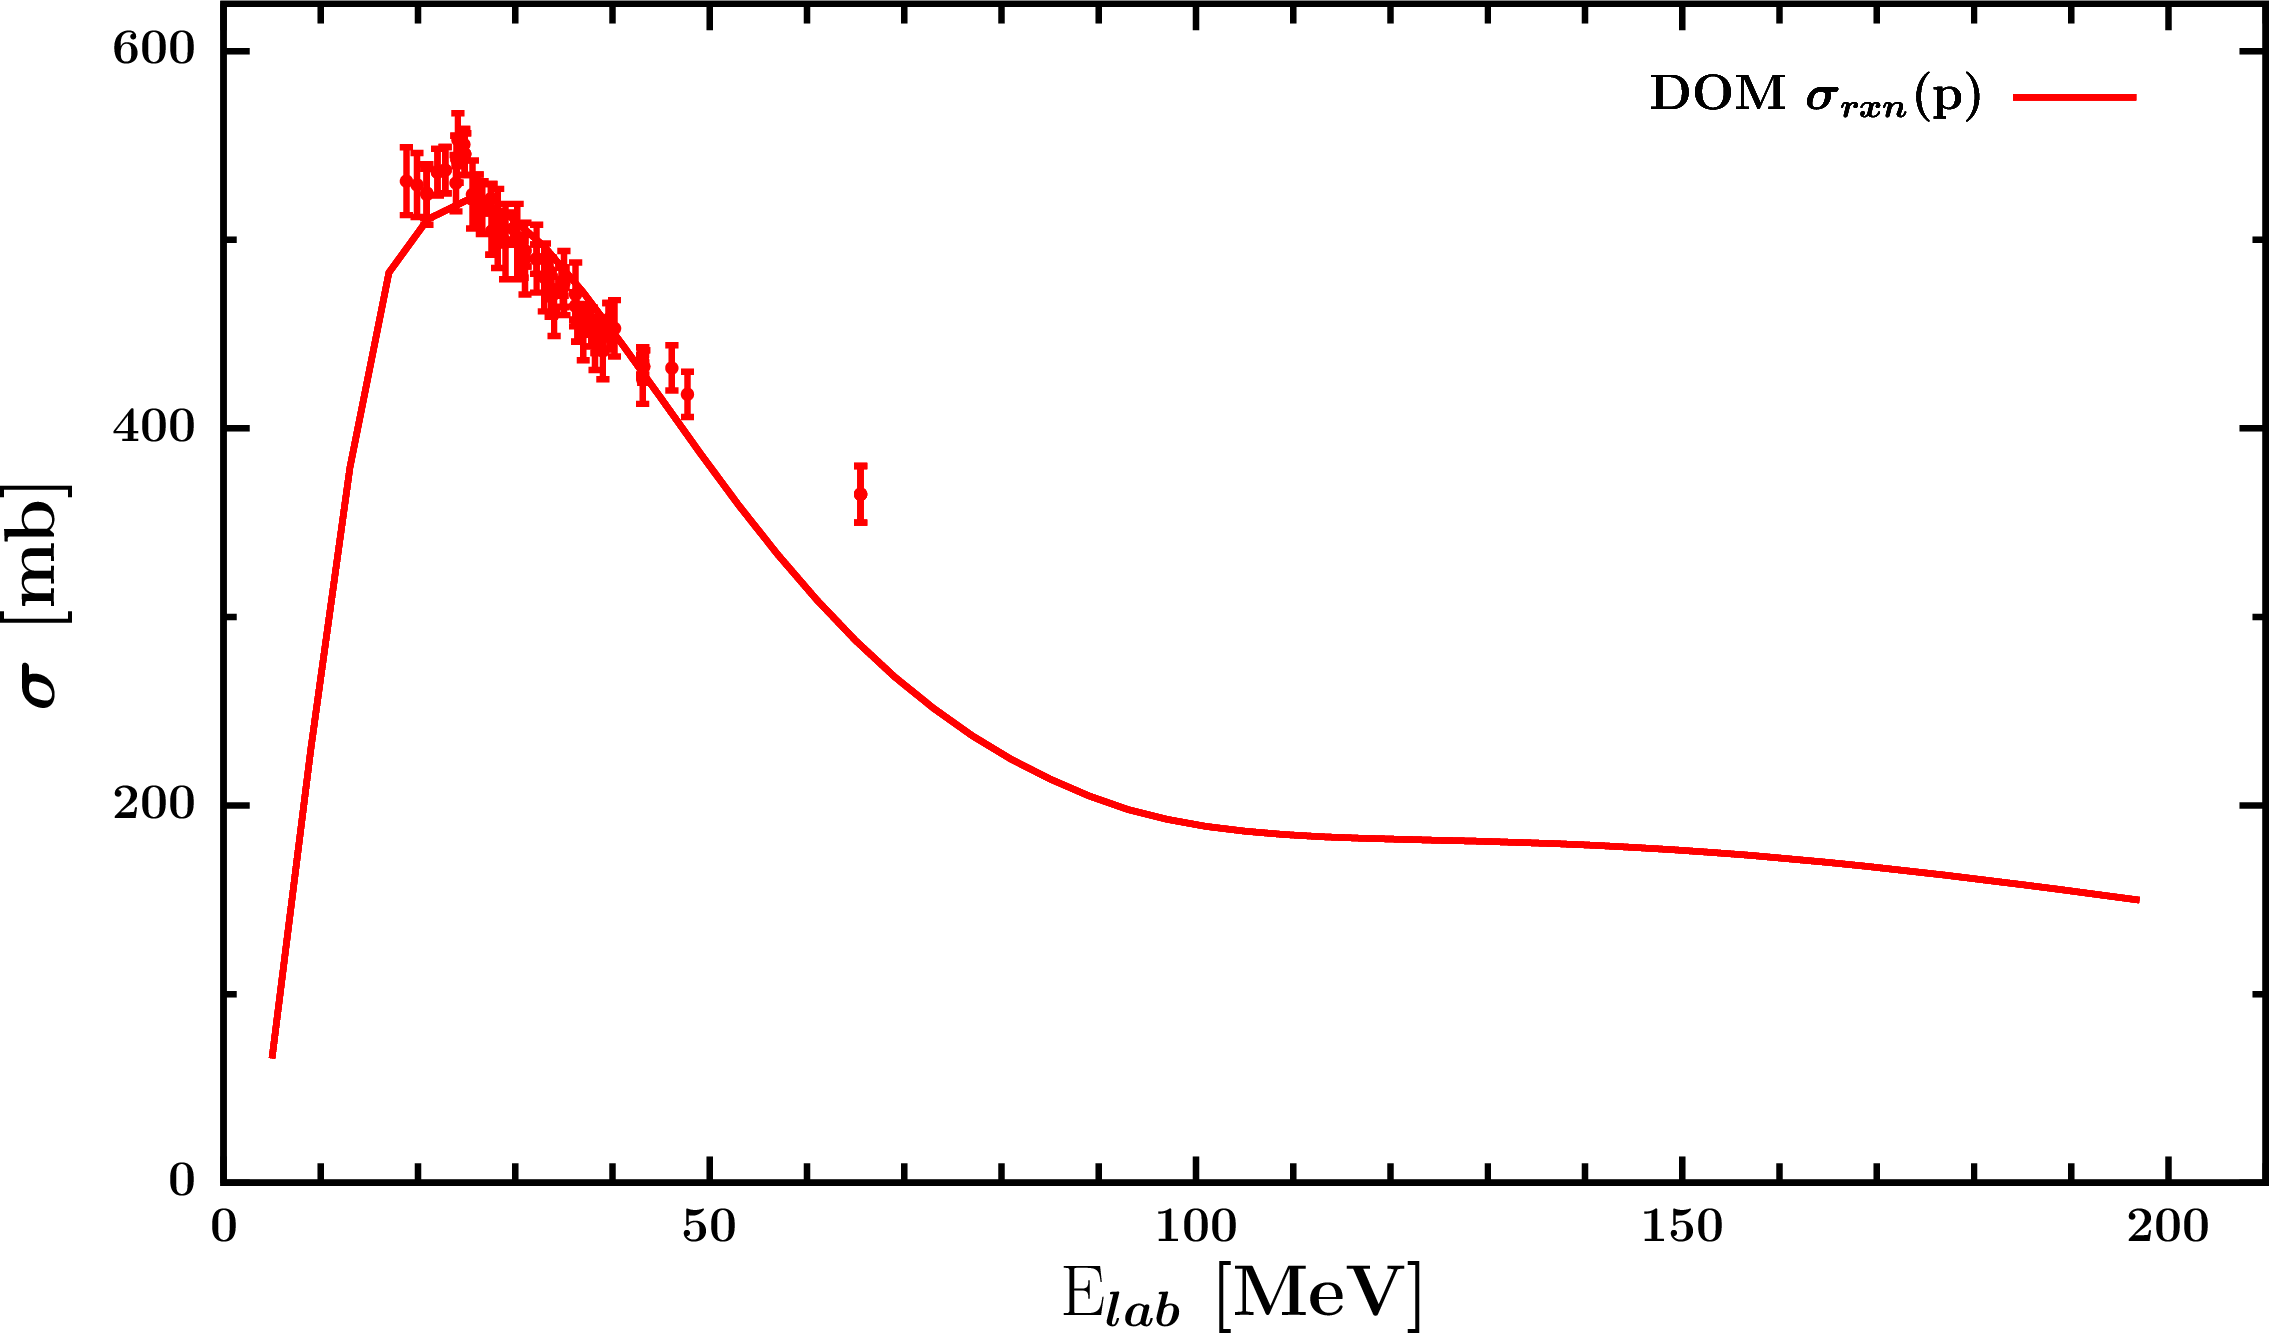
\includegraphics[width=\linewidth]{figures/o16_protonInelastic.png}
        \caption{No \oSix\ proton \rxn\\ data were available}
        \label{DOMFitData_o16_proton_inelastic}
    \end{subfigure}\hspace{6pt}
    \begin{subfigure}[c]{0.45\textwidth}
        \centering
        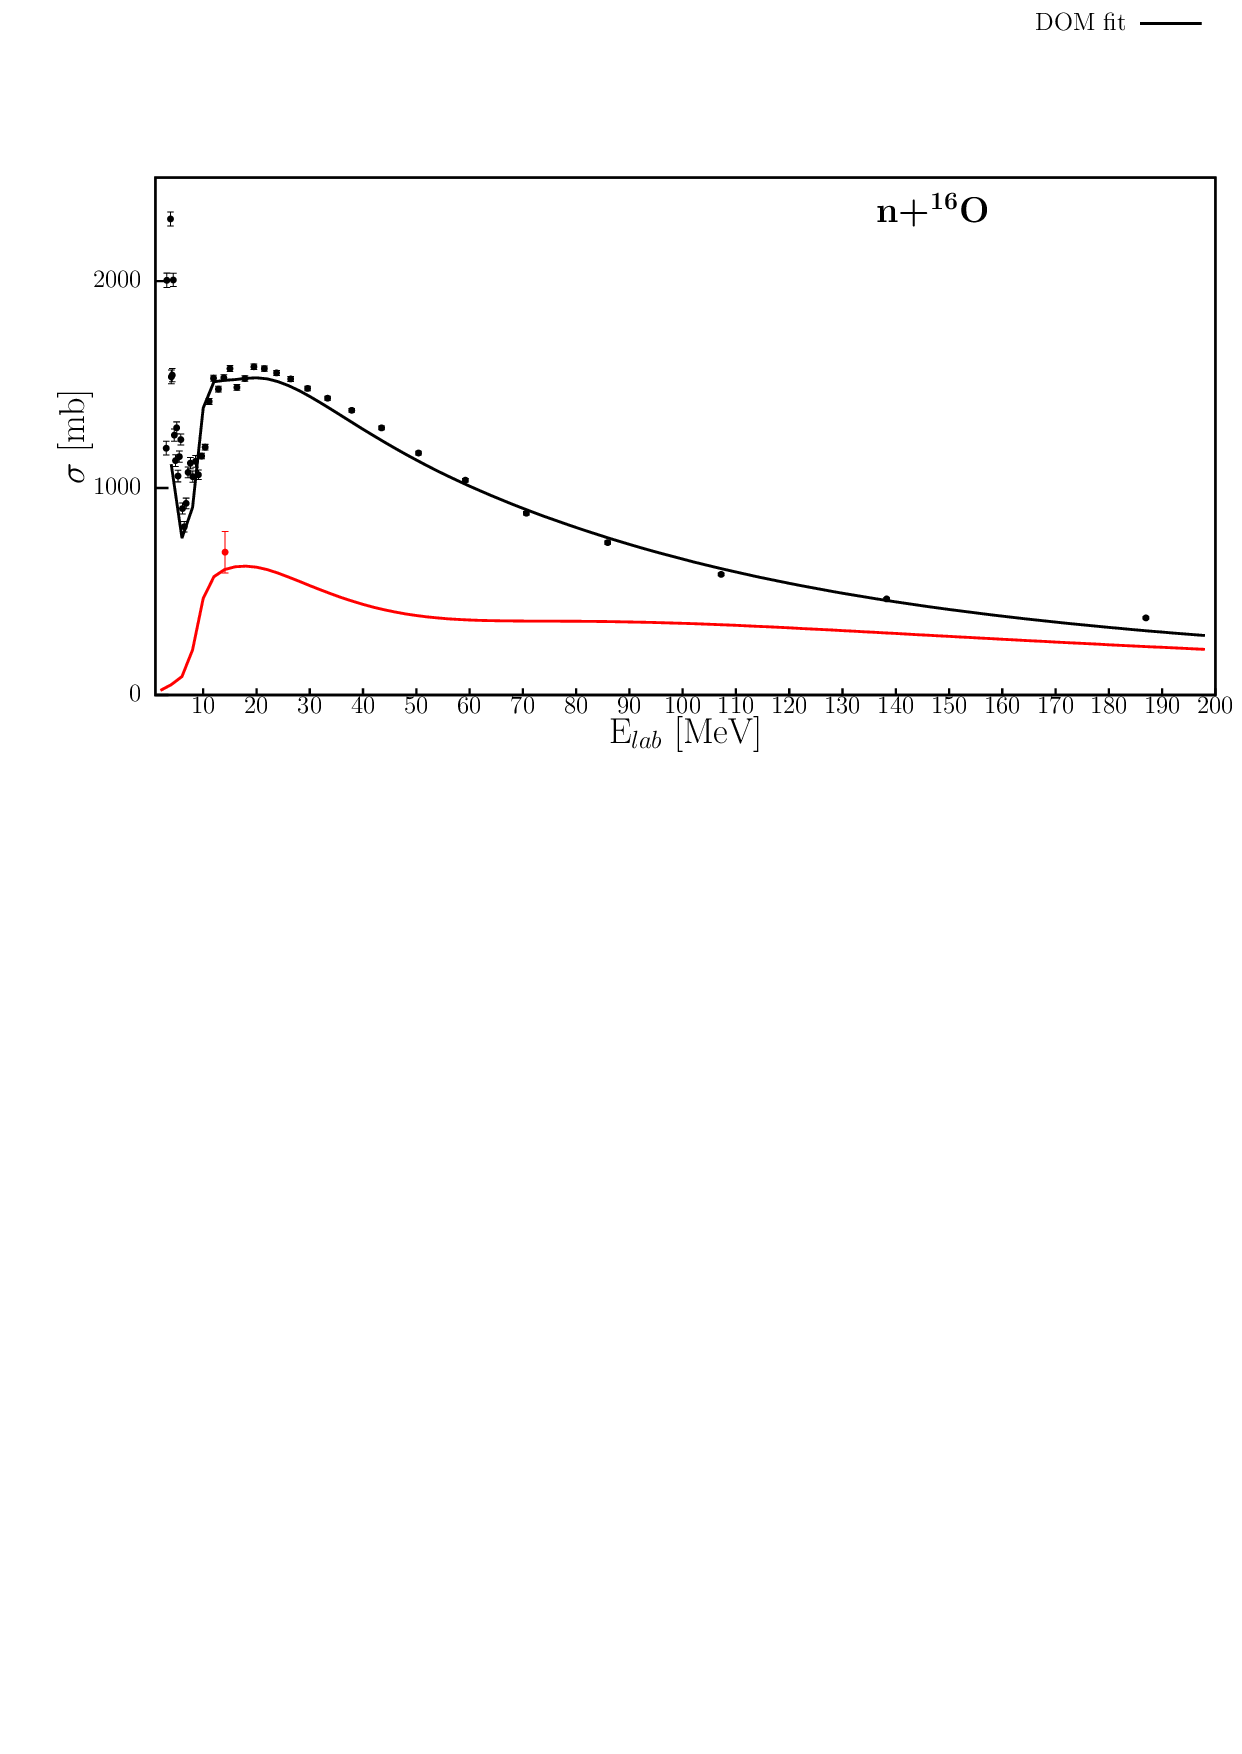
\includegraphics[width=\linewidth]{figures/o16_neutronInelastic.png}
        \caption{\oSix\ neutron \rxn\ and \tot}
        \label{DOMFitData_o16_neutron_inelastic}
    \end{subfigure}
\end{figure}
\afterpage{\clearpage}
\begin{figure}[hbtp]
    \captionsetup[subfigure]{labelformat=empty}
    \centering
    \begin{subfigure}[b]{0.45\textwidth}
        \centering
        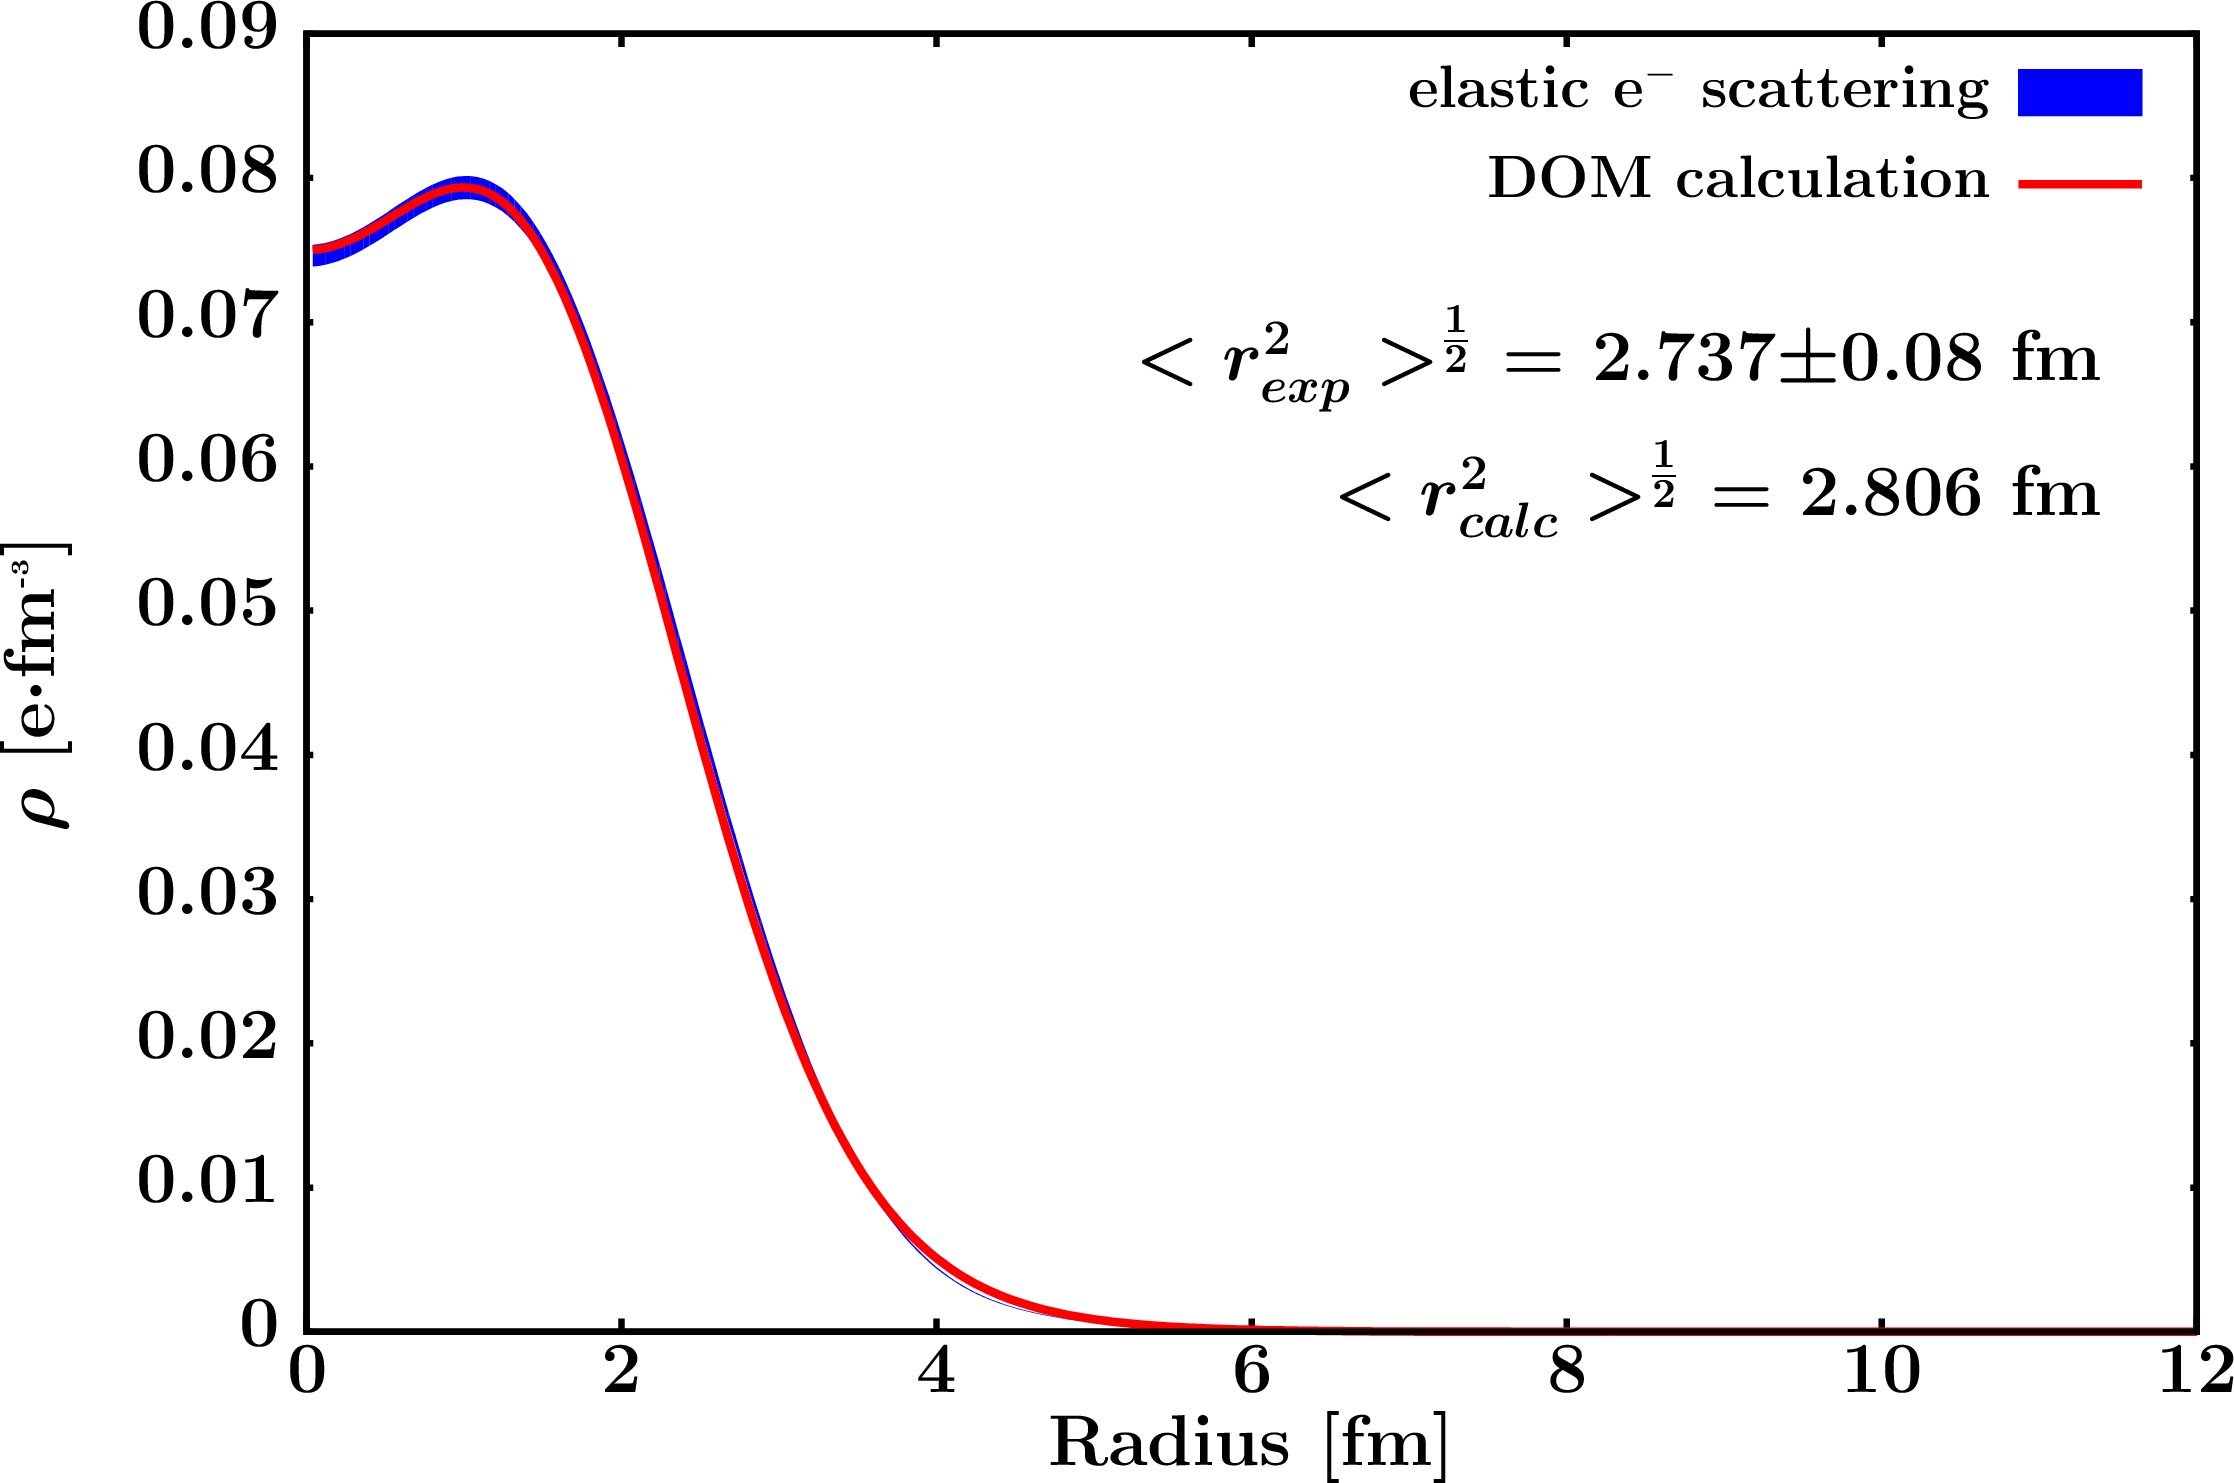
\includegraphics[width=\linewidth]{figures/o16_chargeDensity.png}
        \caption{\oSix\ charge density}
        \label{DOMFitData_o16_chargeDensity}
    \end{subfigure}\hspace{6pt}
    \begin{subfigure}[b]{0.45\textwidth}
        \centering
        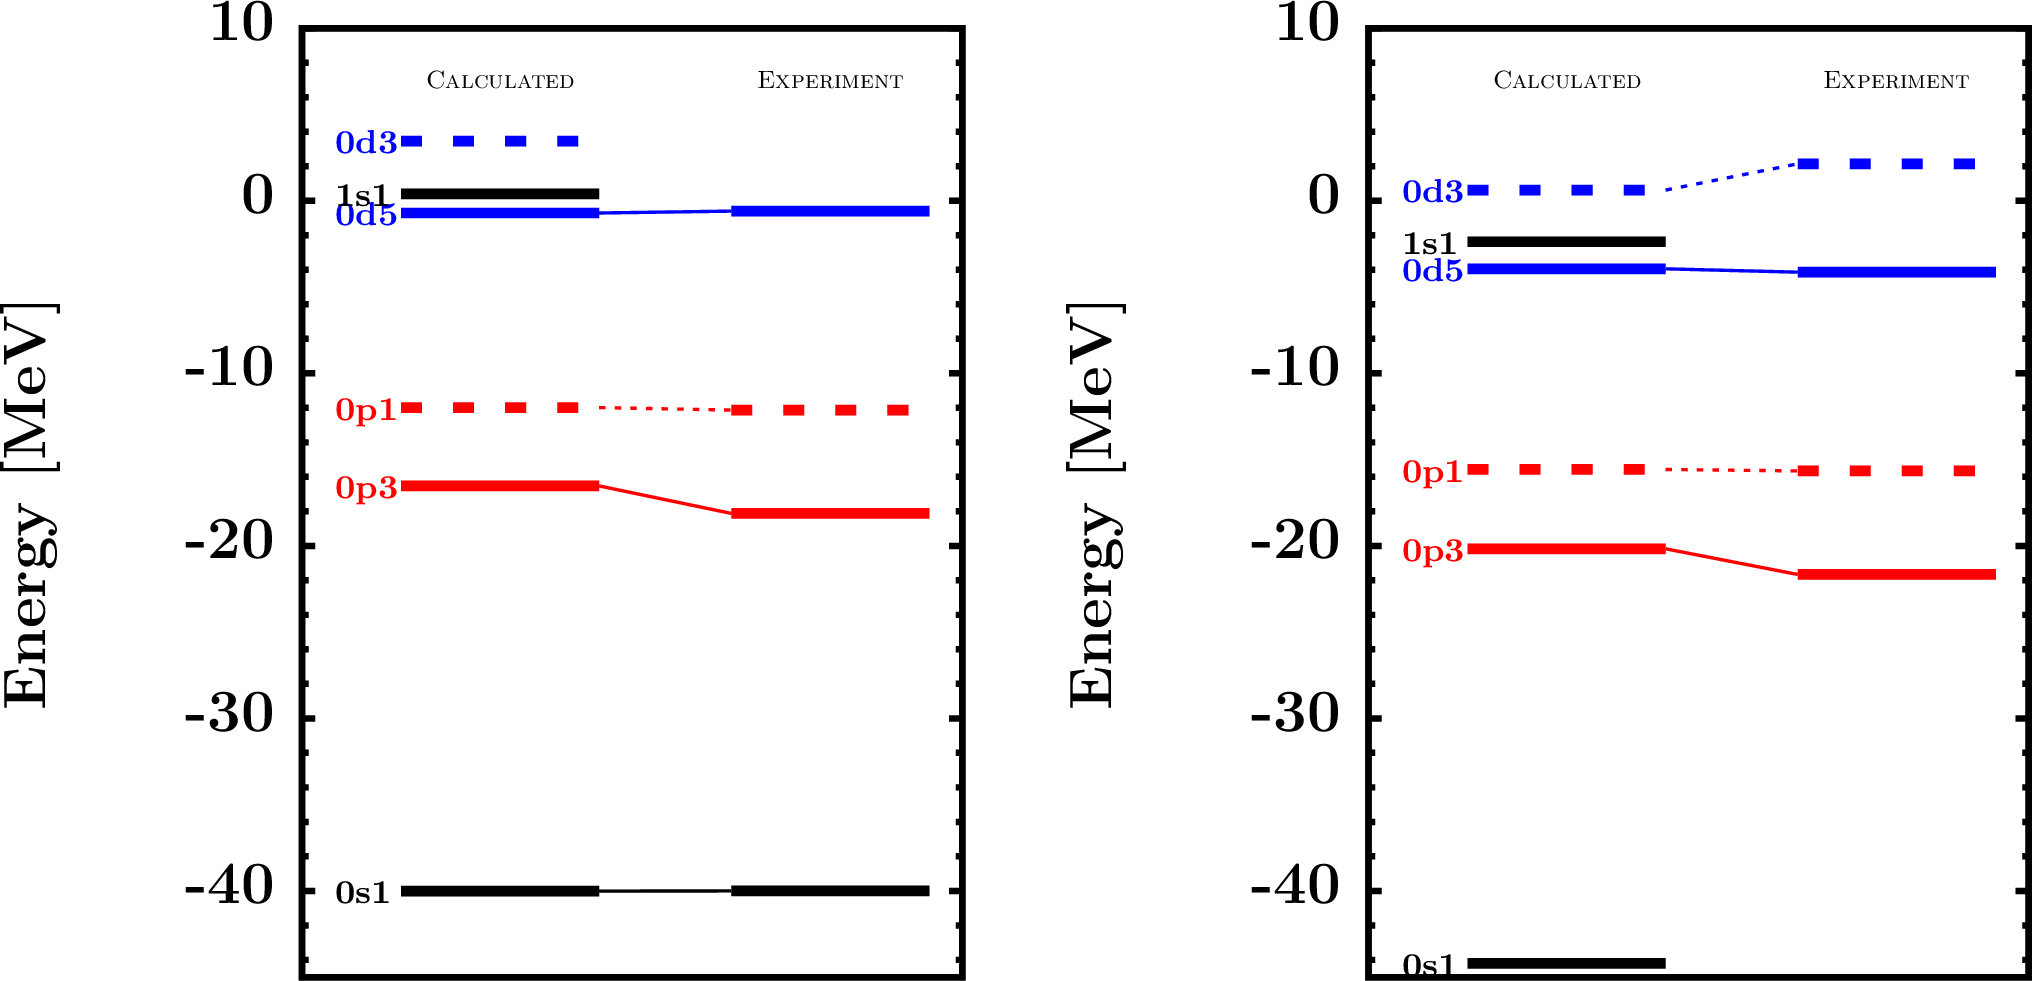
\includegraphics[width=\linewidth]{figures/o16_SPLevels.png}
        \caption{\oSix\ single-particle levels}
        \label{DOMFitData_o16_SPLevels}
    \end{subfigure}\vspace{0.3in}
    \begin{subfigure}[b]{0.45\textwidth}
        \centering
        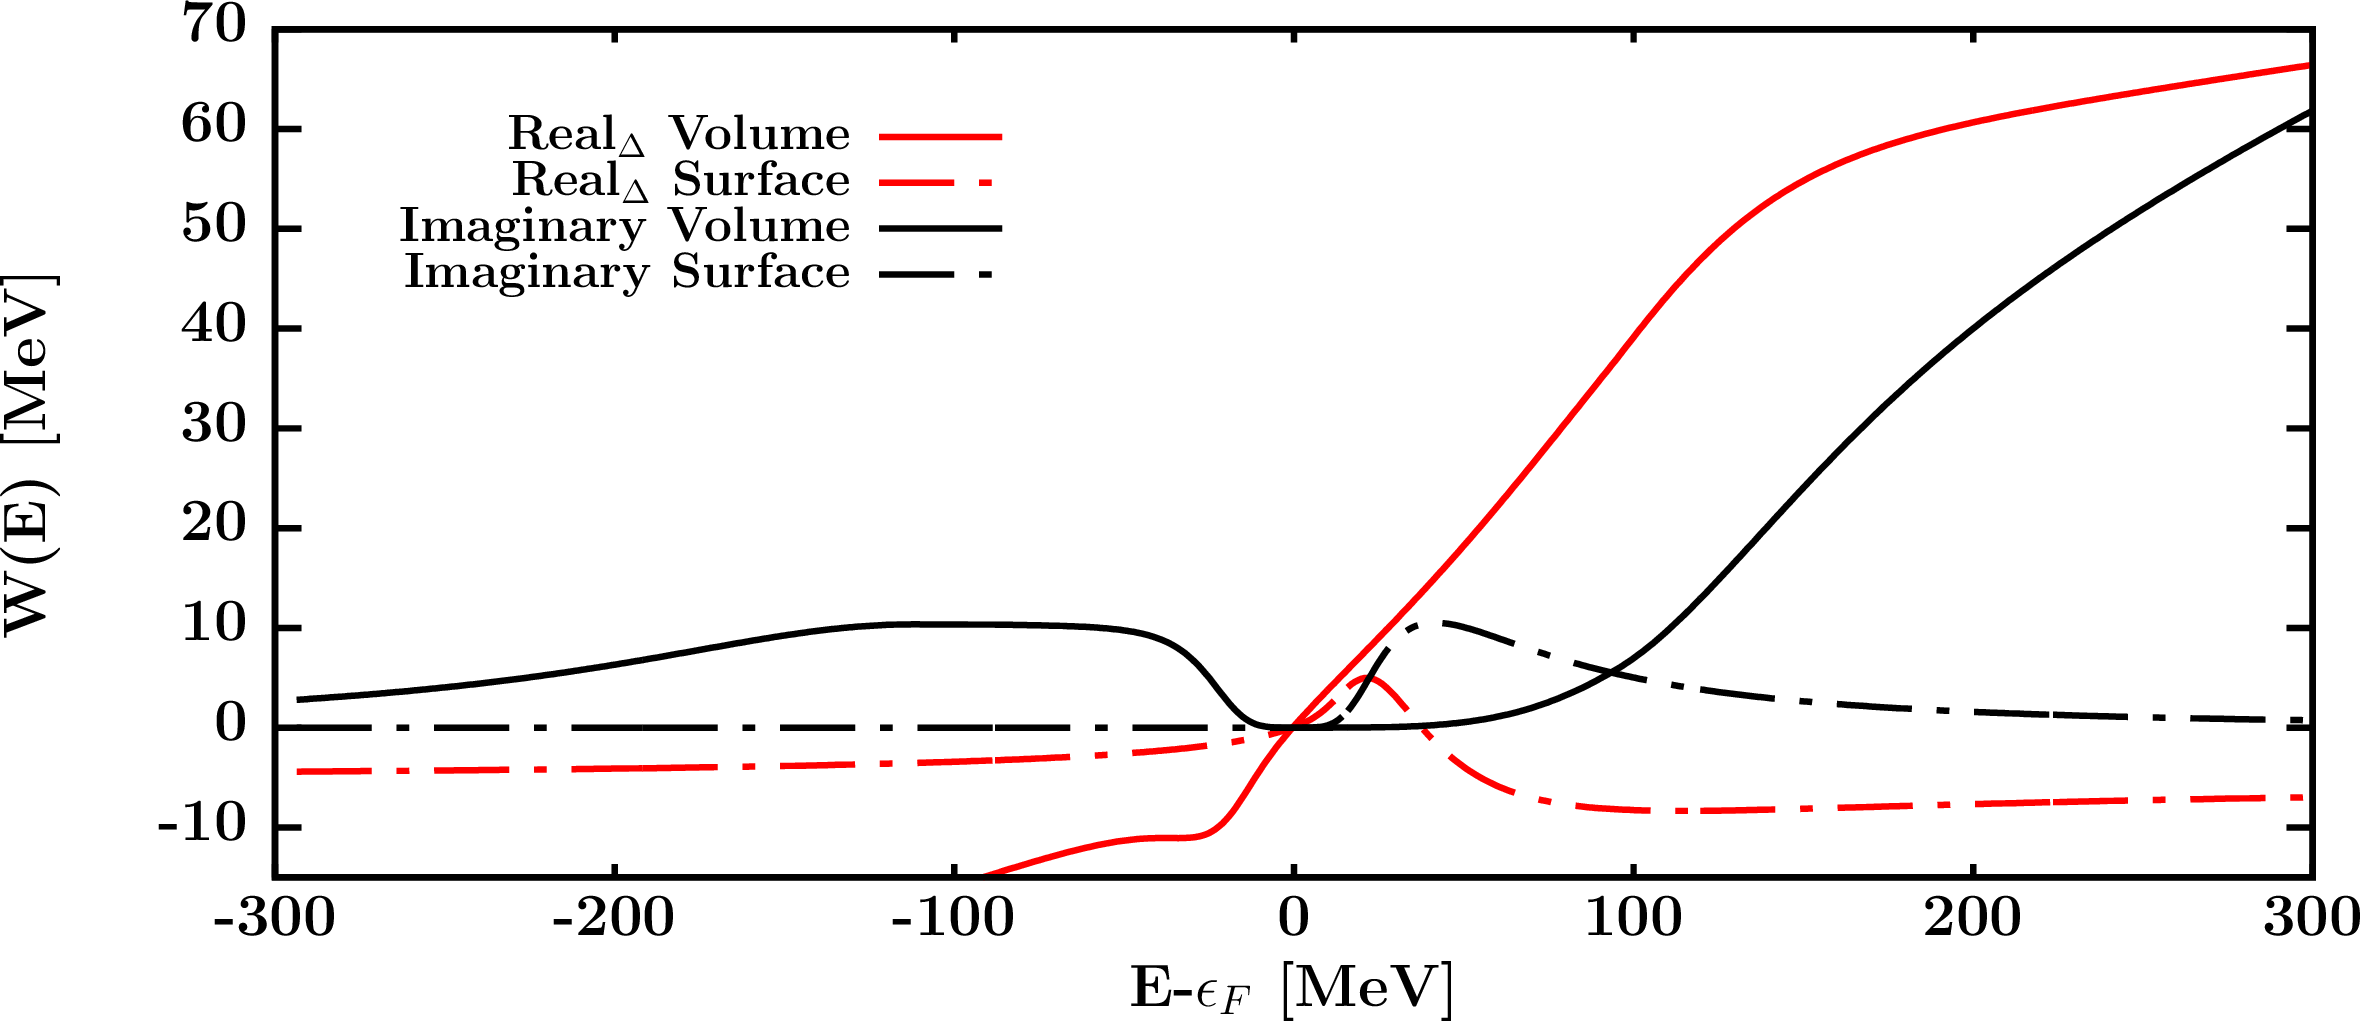
\includegraphics[width=\linewidth]{figures/o16_protonPotentials.png}
        \caption{\oSix\ proton potential energy-dependence}
        \label{DOMFitData_o16_proton_potentialComponent_energy}
    \end{subfigure}\hspace{6pt}
    \begin{subfigure}[b]{0.45\linewidth}
        \centering
        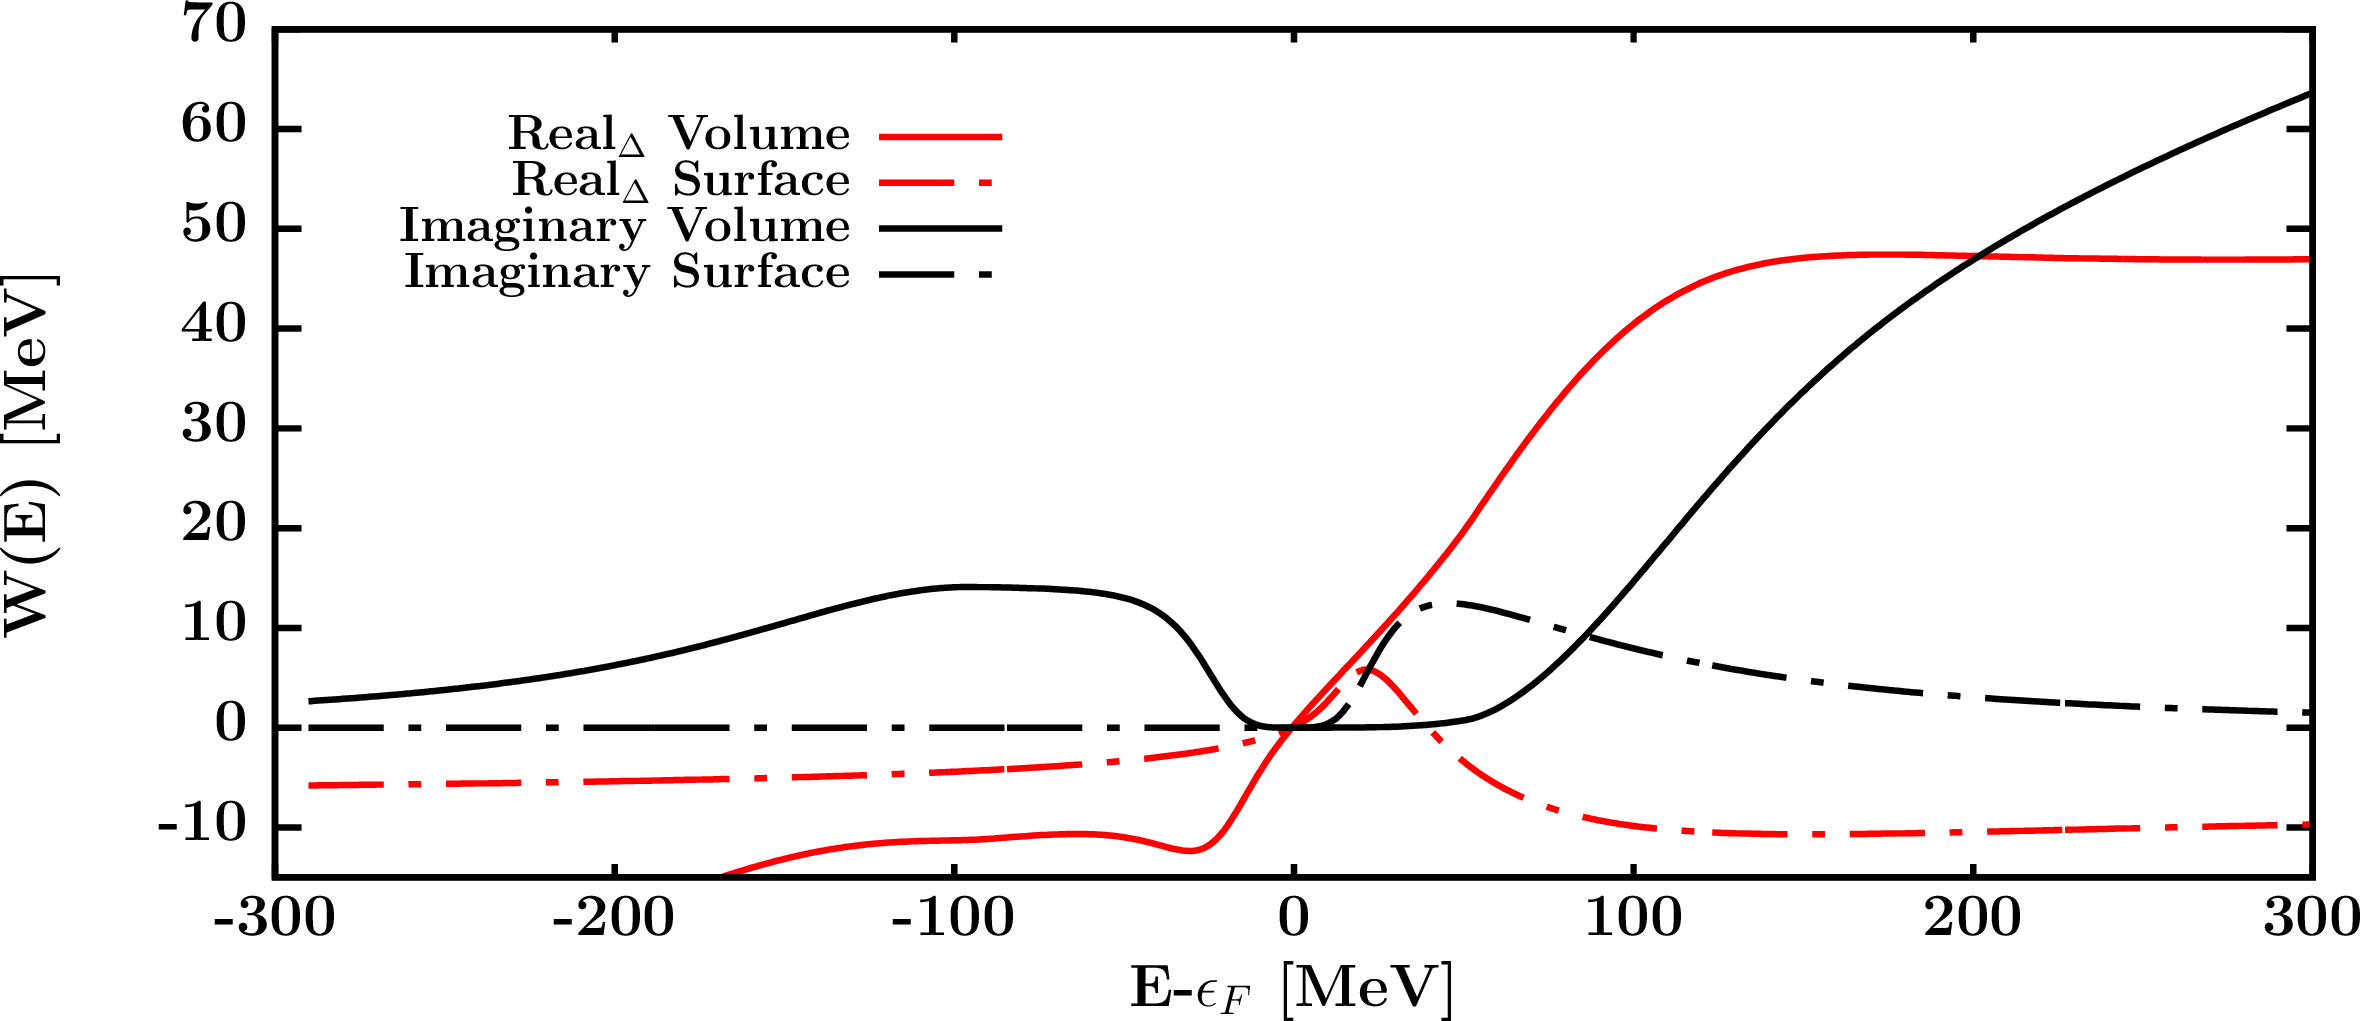
\includegraphics[width=\linewidth]{figures/o16_neutronPotentials.png}
        \caption{\oSix\ neutron potential energy-dependence}
        \label{DOMFitData_o16_neutron_potentialComponent_energy}
    \end{subfigure}\vspace{0.3in}
    \begin{subfigure}[b]{0.45\textwidth}
        \centering
        
\includegraphics[width=\linewidth]{figures/o16_protonVolumeIntegrals.png}
        \caption{\oSix\ proton volume integral}
        \label{DOMFitData_o16_proton_potentialIntegral}
    \end{subfigure}\hspace{6pt}
    \begin{subfigure}[b]{0.45\textwidth}
        \centering
        
\includegraphics[width=\linewidth]{figures/o16_neutronVolumeIntegrals.png}
        \caption{\oSix\ neutron volume integral}
        \label{DOMFitData_o16_neutron_potentialIntegral}
    \end{subfigure}\vspace{0.3in}
    \begin{subfigure}[b]{0.45\textwidth}
        \centering
        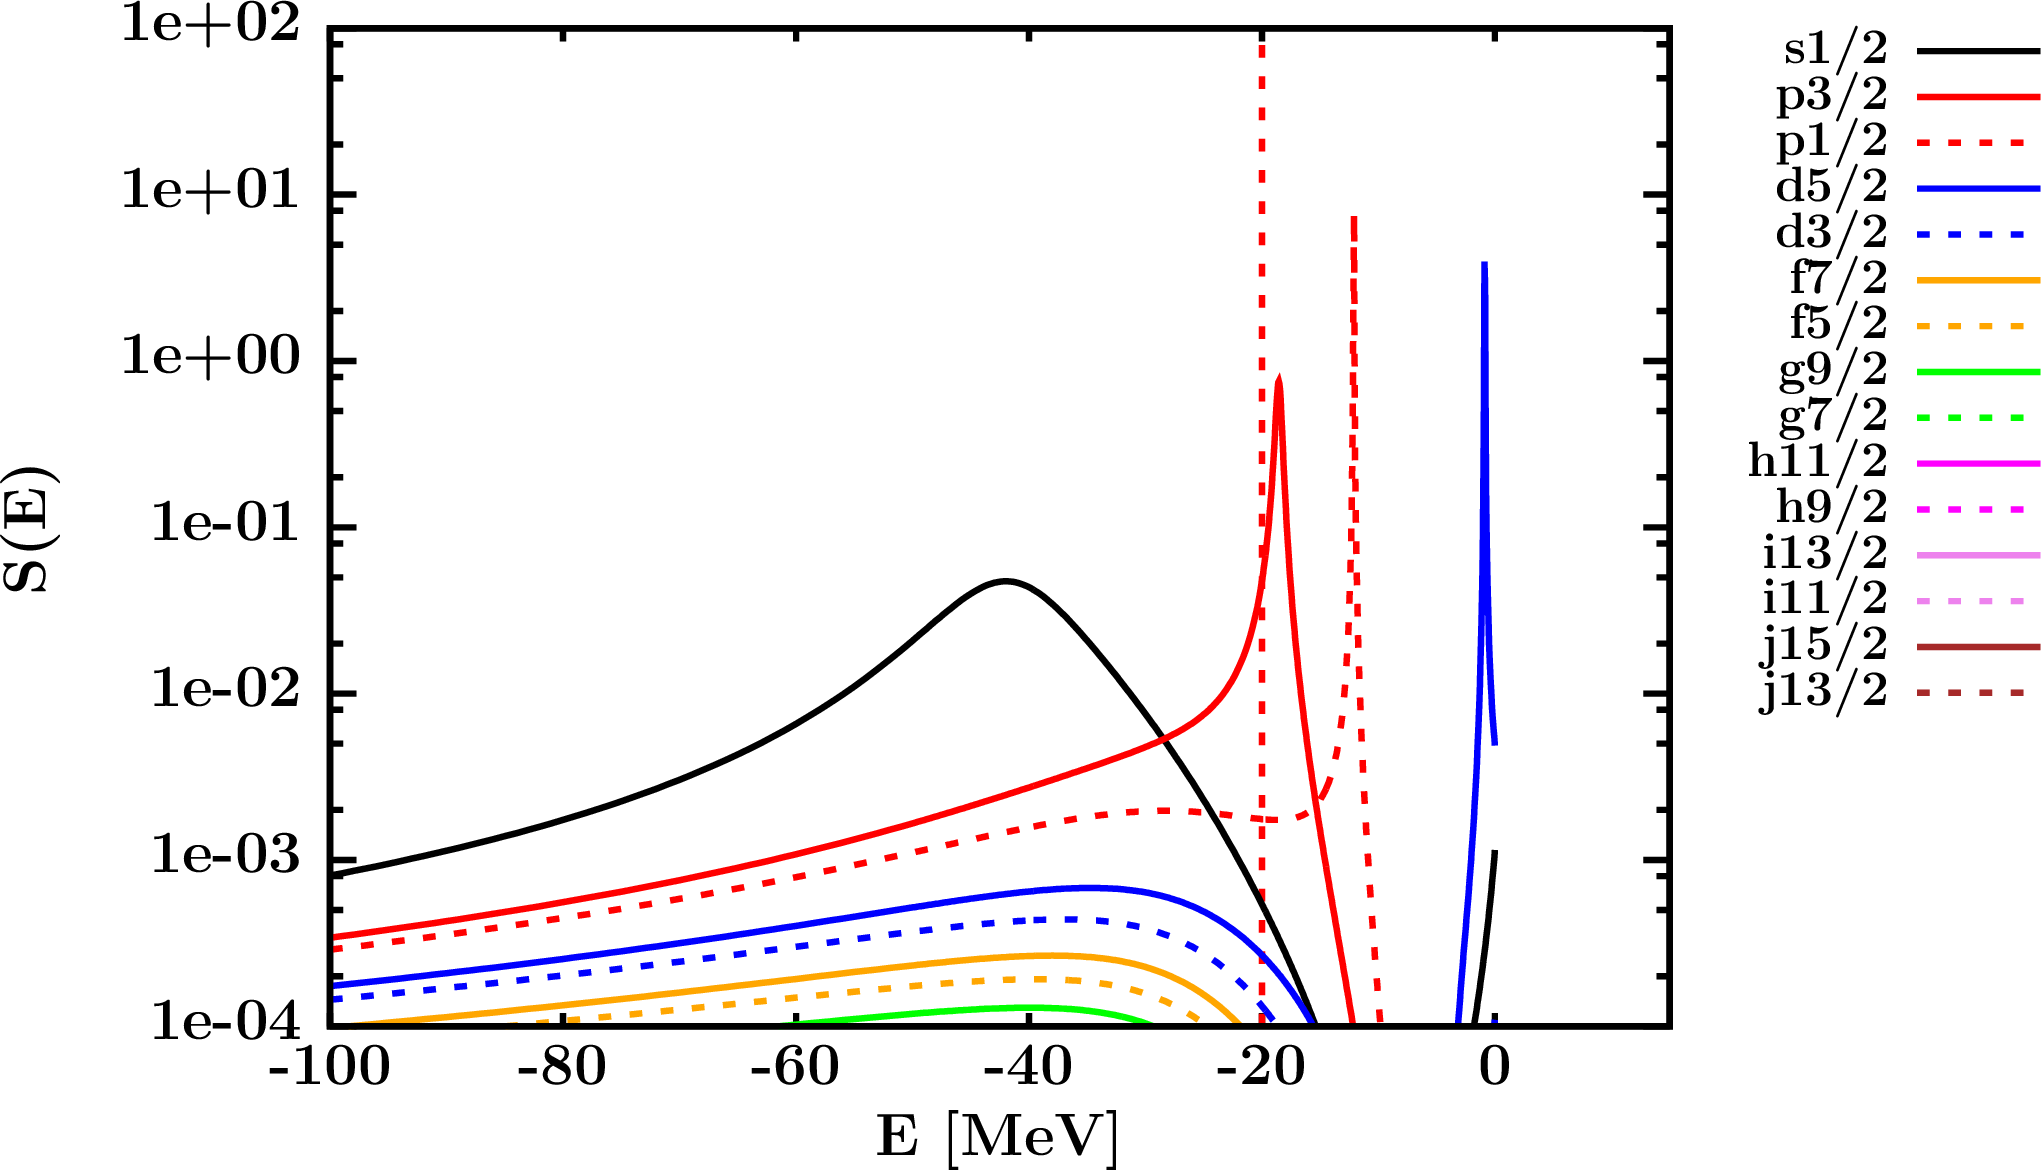
\includegraphics[width=\linewidth]{figures/o16_protonSpectralFunctions.png}
        \caption{\oSix\ proton spectral functions}
        \label{DOMFitData_o16_proton_spectralFunctions}
    \end{subfigure}\hspace{6pt}
    \begin{subfigure}[b]{0.45\textwidth}
        \centering
        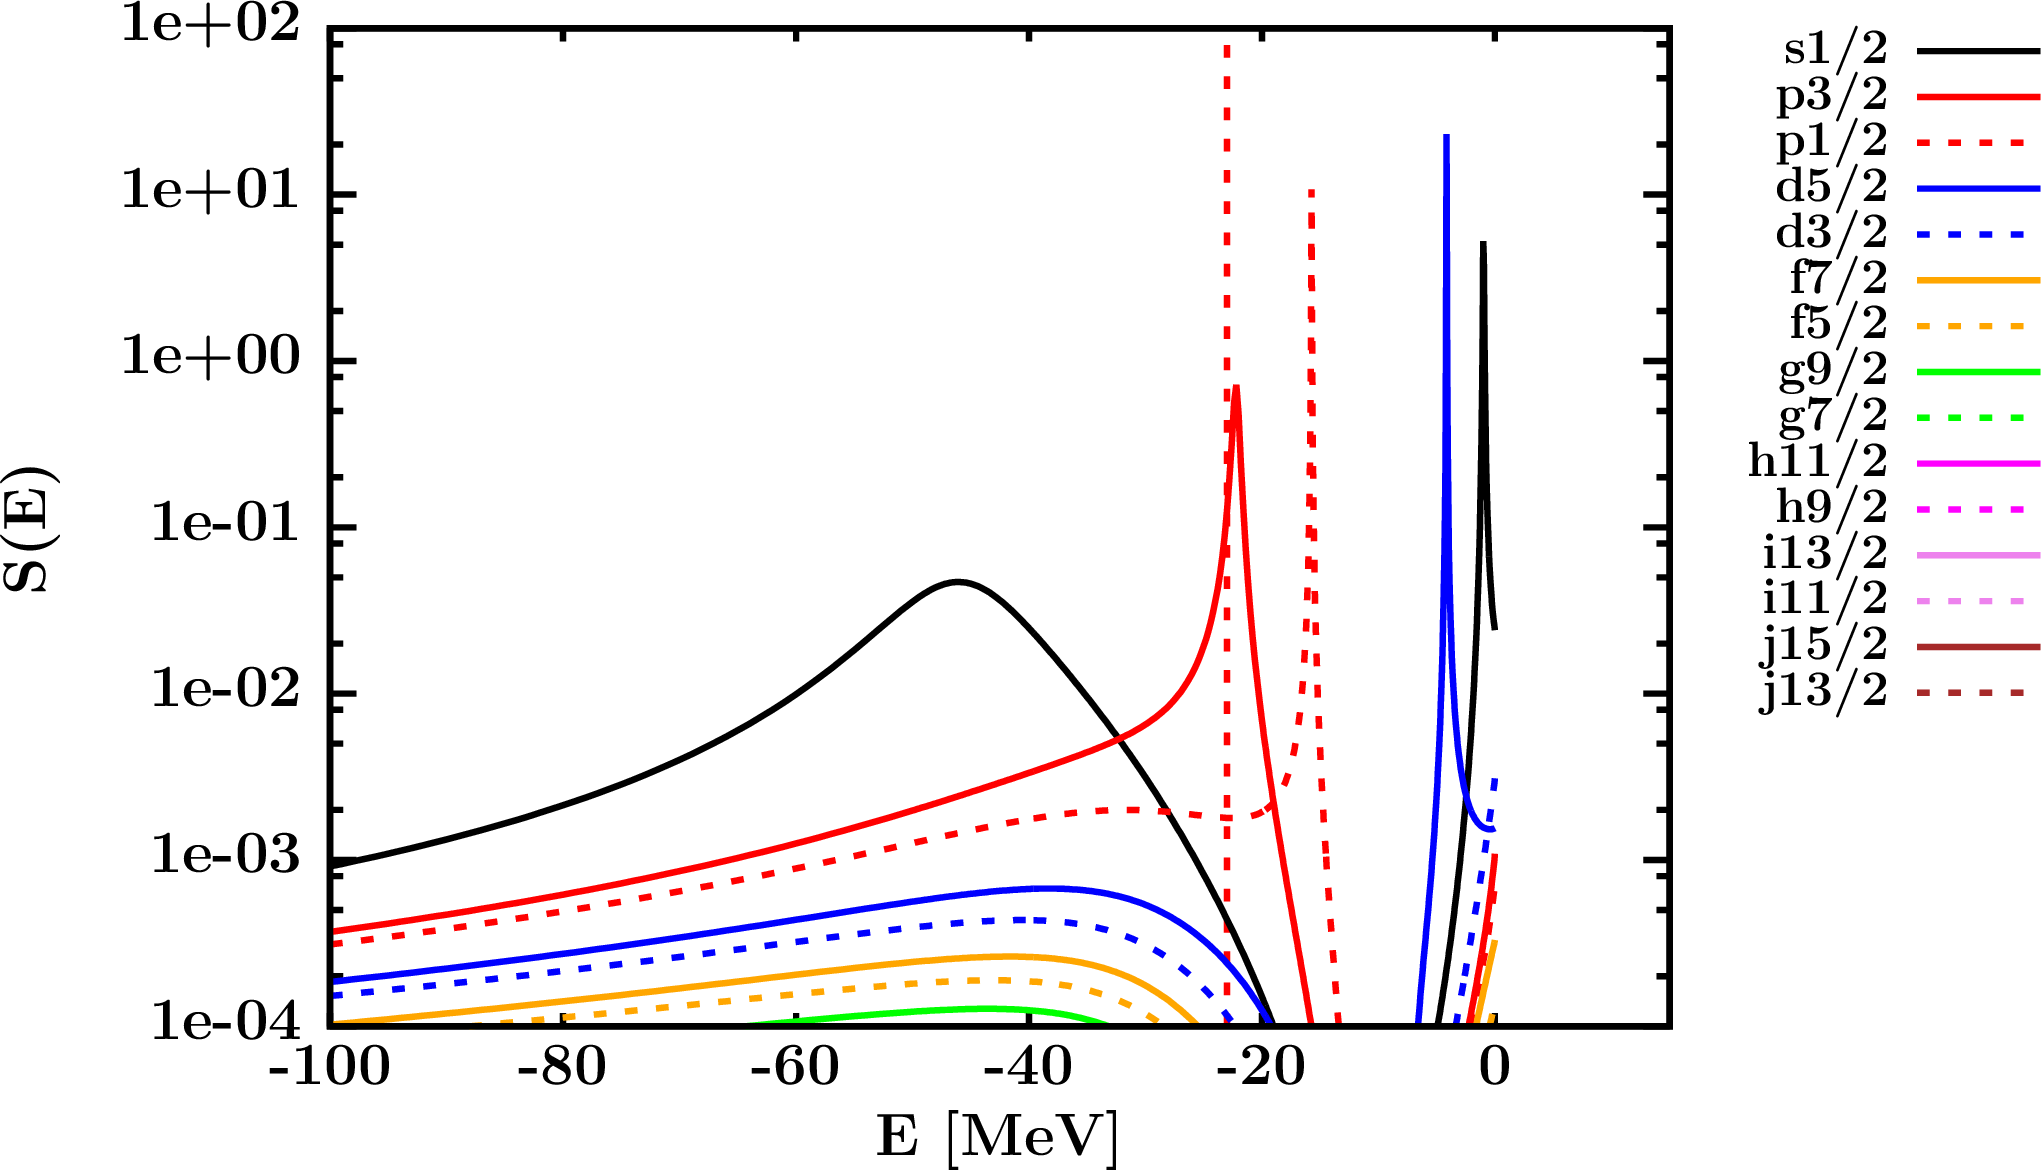
\includegraphics[width=\linewidth]{figures/o16_neutronSpectralFunctions.png}
        \caption{\oSix\ neutron spectral functions}
        \label{DOMFitData_o16_neutron_spectralFunctions}
    \end{subfigure}
\end{figure}
\afterpage{\clearpage}
\begin{figure}[hbtp]
    \captionsetup[subfigure]{labelformat=empty}
    \centering
    \begin{subfigure}[b]{0.45\textwidth}
        \centering
        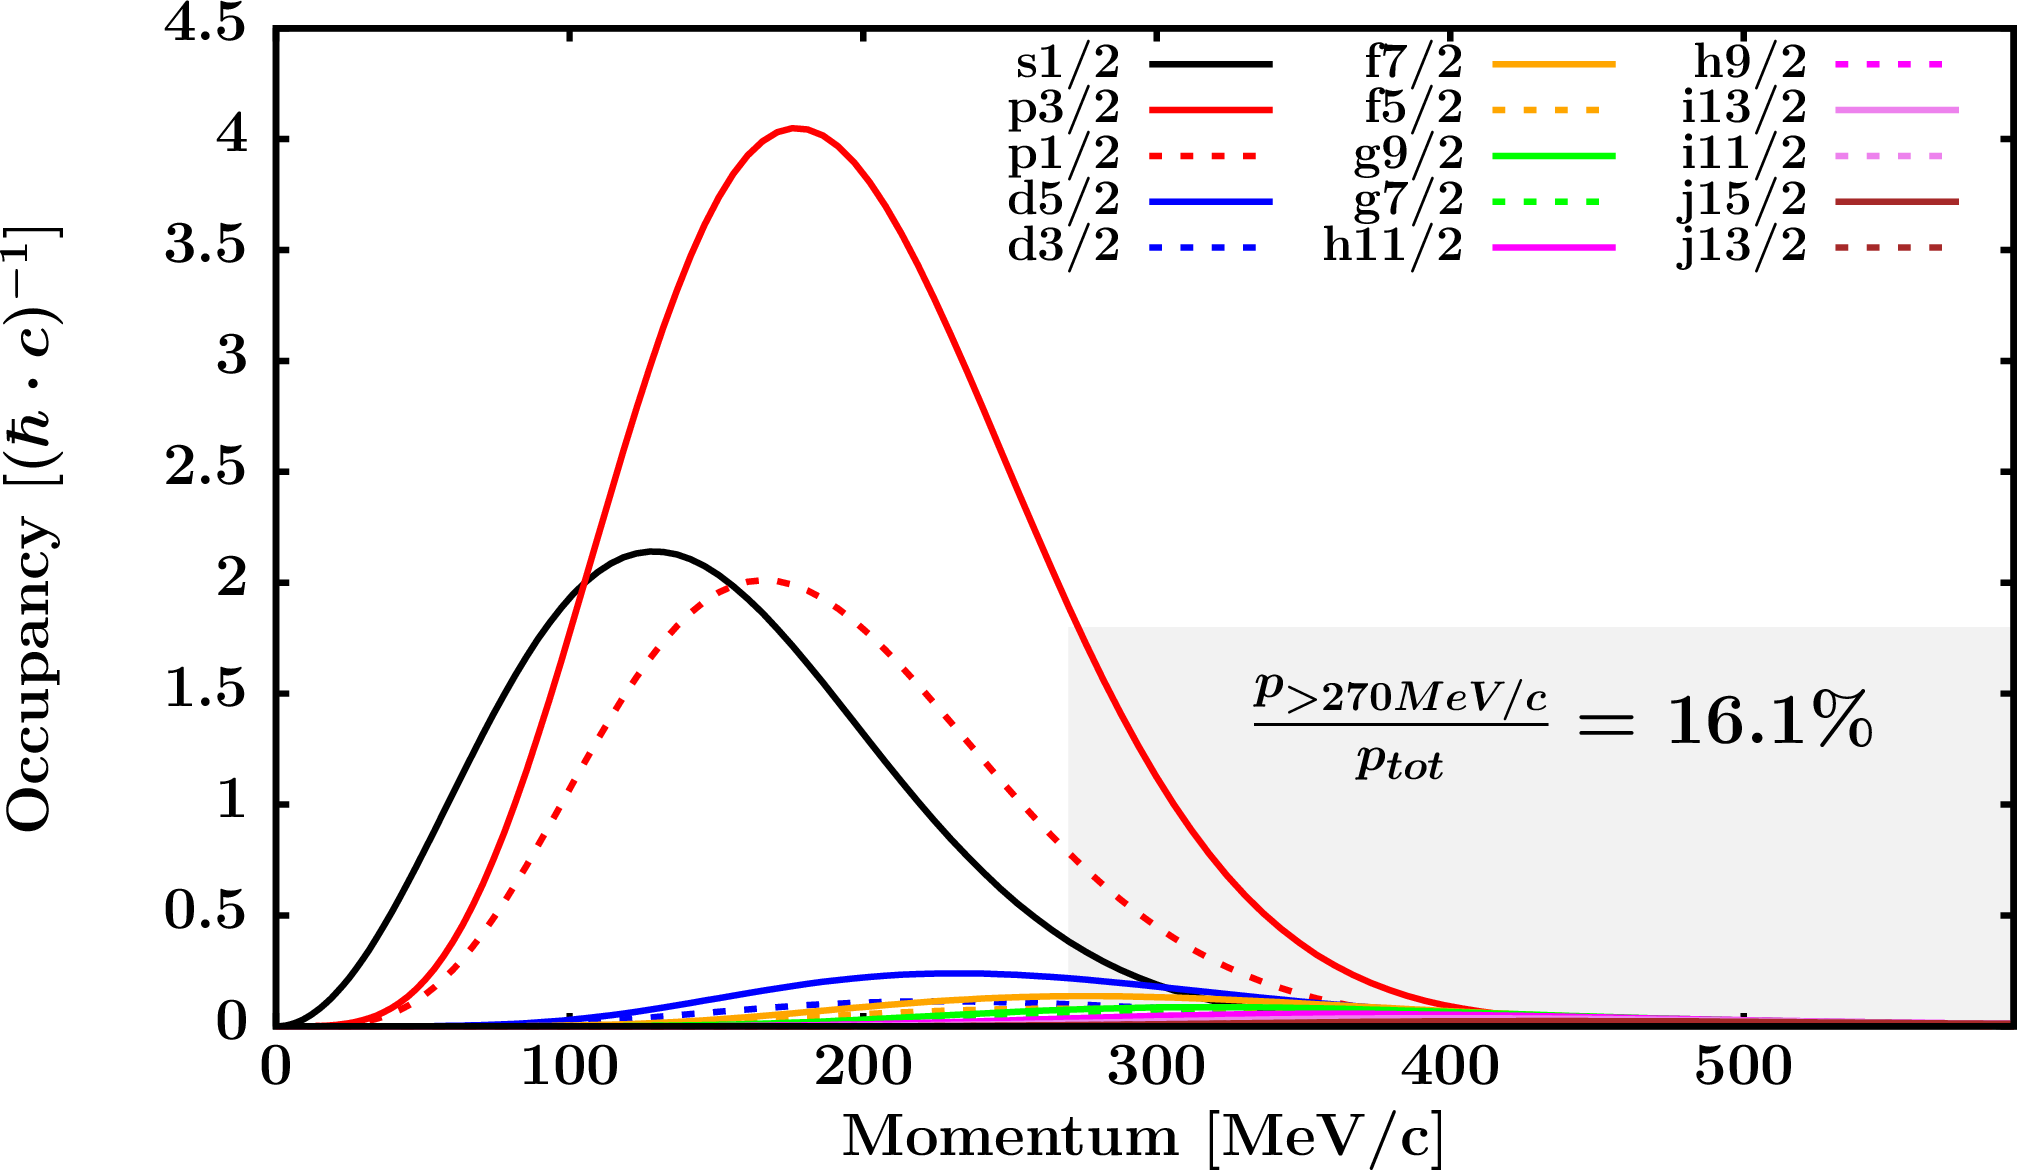
\includegraphics[width=\linewidth]{figures/o16_protonLJMomentumDistIntegral.png}
        \caption{\oSix\ proton momentum distribution}
        \label{DOMFitData_o16_proton_momentumDist}
    \end{subfigure}\hspace{6pt}
    \begin{subfigure}[b]{0.45\textwidth}
        \centering
        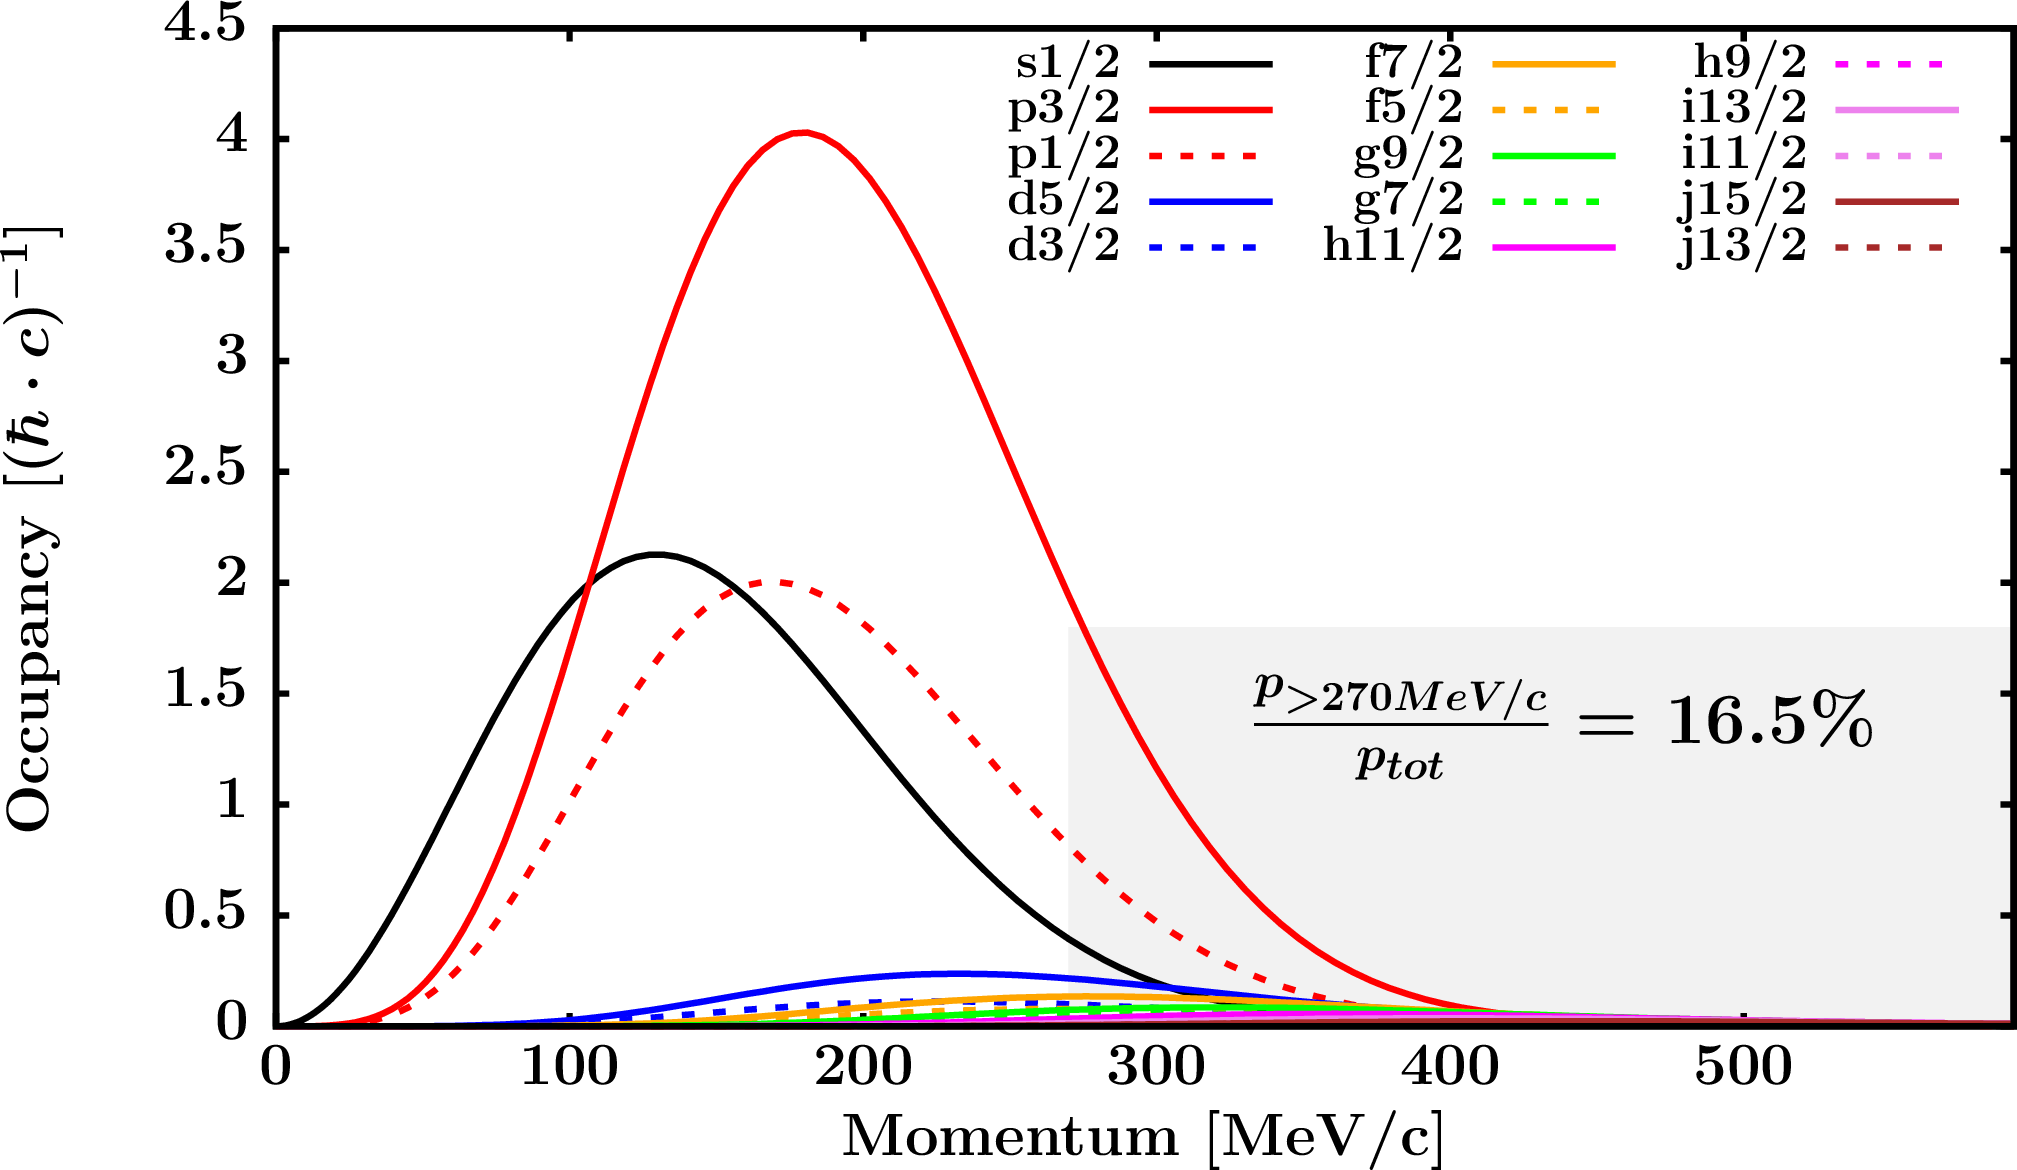
\includegraphics[width=\linewidth]{figures/o16_neutronLJMomentumDistIntegral.png}
        \caption{\oSix\ neutron momentum distribution}
        \label{DOMFitData_o16_neutron_momentumDist}
    \end{subfigure}\vspace{0.3in}
    \begin{subfigure}{0.45\textwidth}
        \centering
        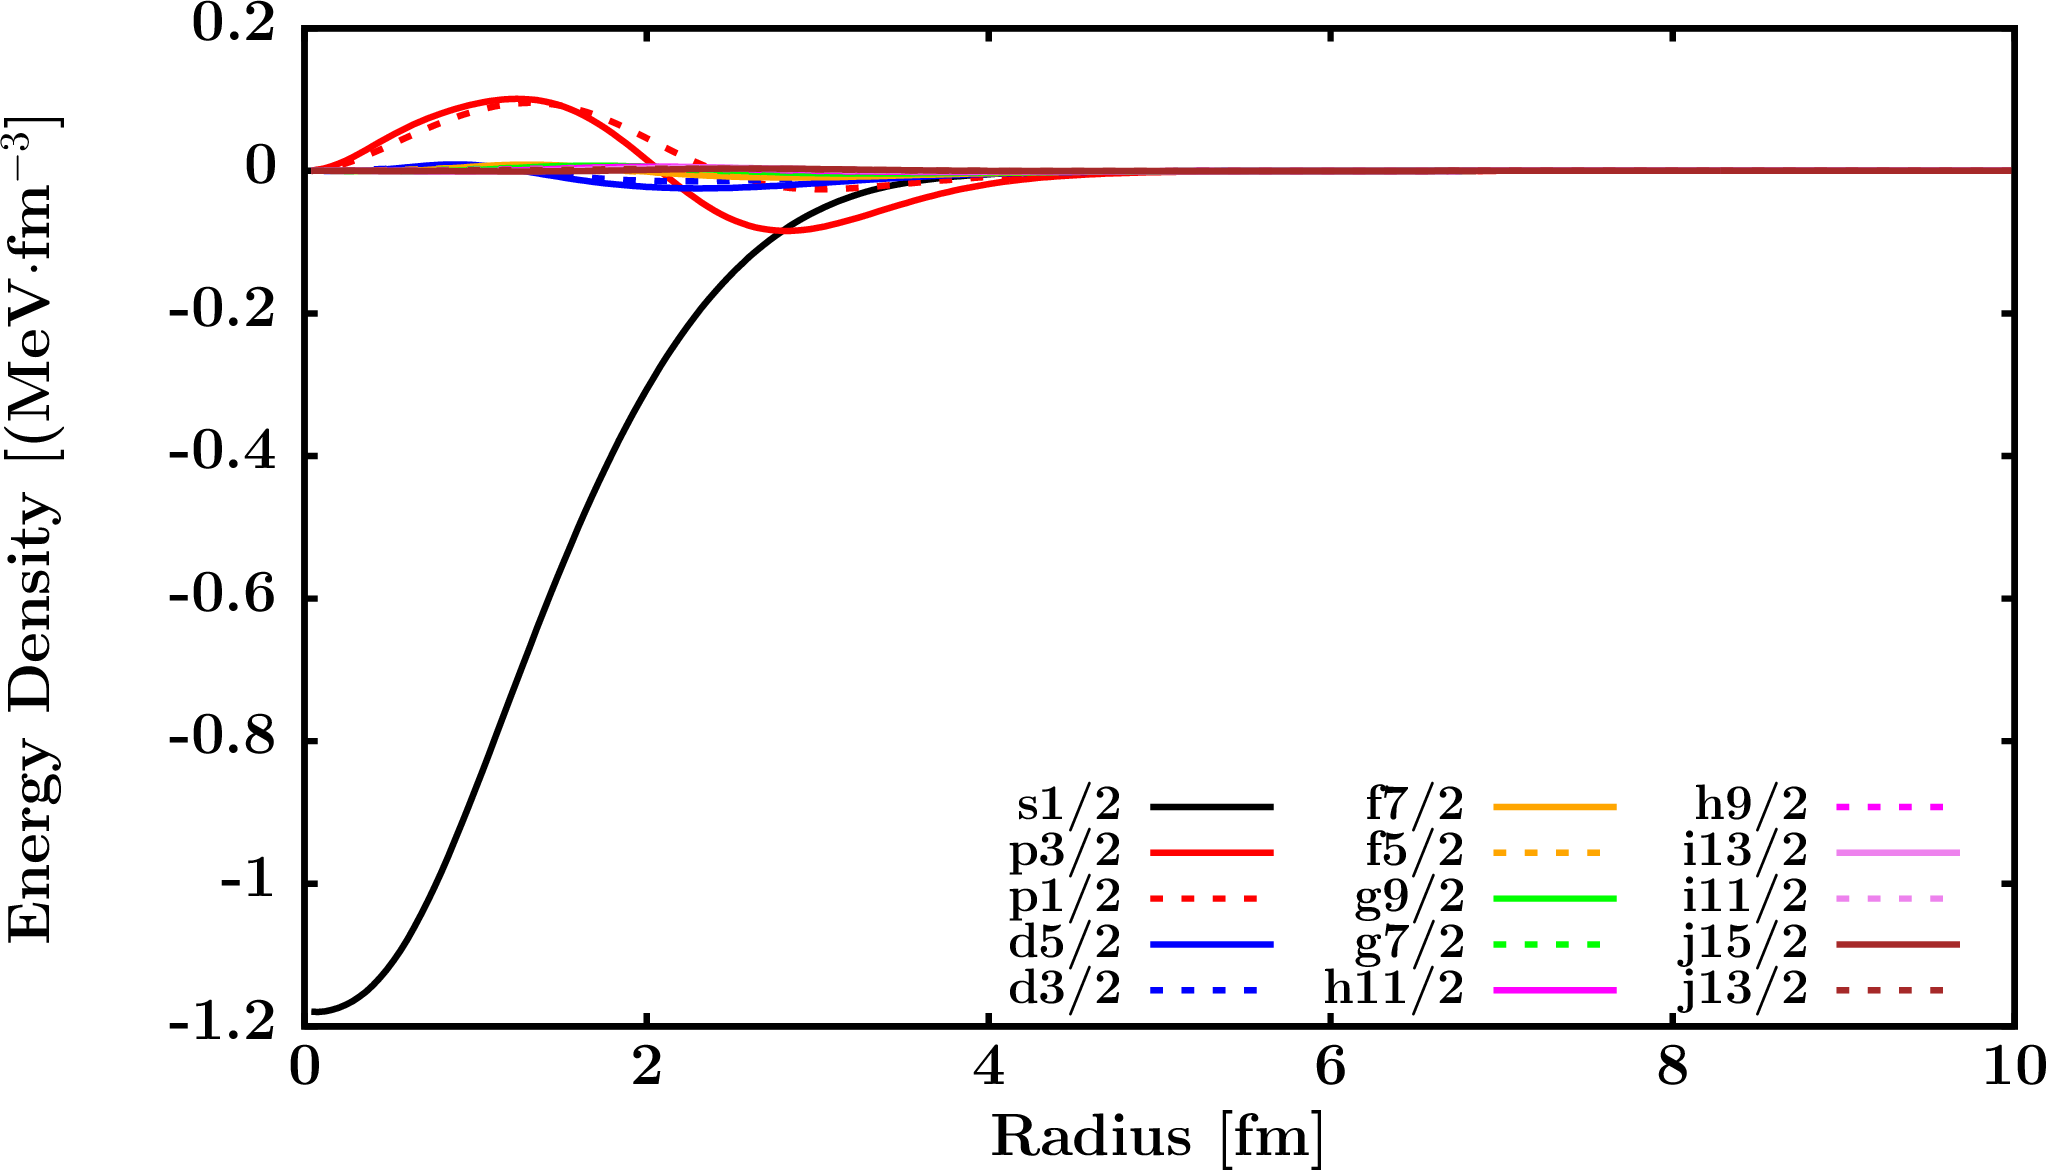
\includegraphics[width=\linewidth]{figures/o16_EnergyDist.png}
        \caption{\oSix\ energy distribution by LJ}
        \label{DOMFitData_o16_proton_energyDistInt}
    \end{subfigure}\hspace{6pt}
    \begin{subfigure}{0.45\textwidth}
        \centering
        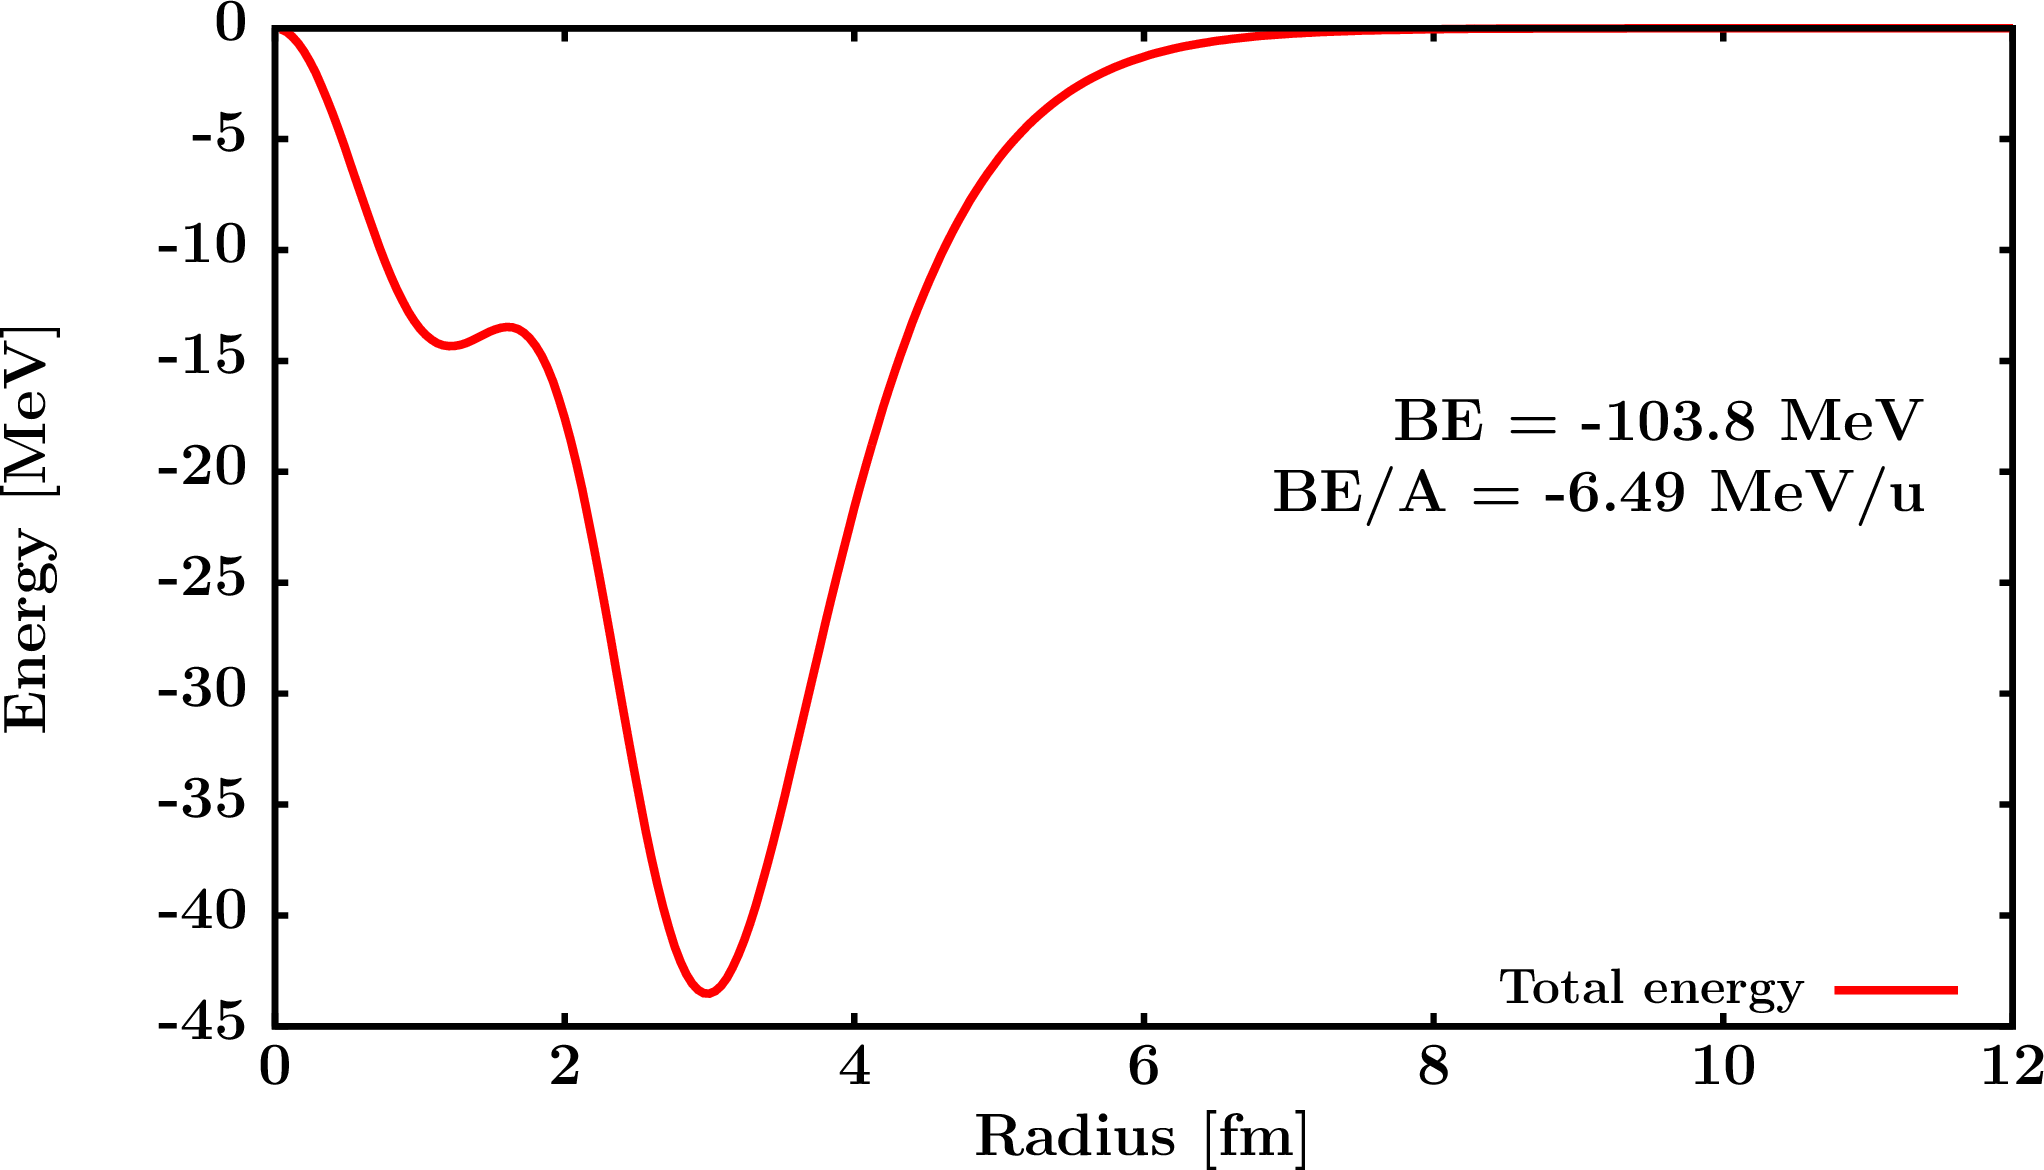
\includegraphics[width=\linewidth]{figures/o16_EnergyDistIntegral.png}
        \caption{\oSix\ energy distribution integral}
        \label{DOMFitData_o16_neutron_energyDistInt}
    \end{subfigure}\vspace{0.4in}
    \begin{subfigure}{0.70\textwidth}
        \centering
        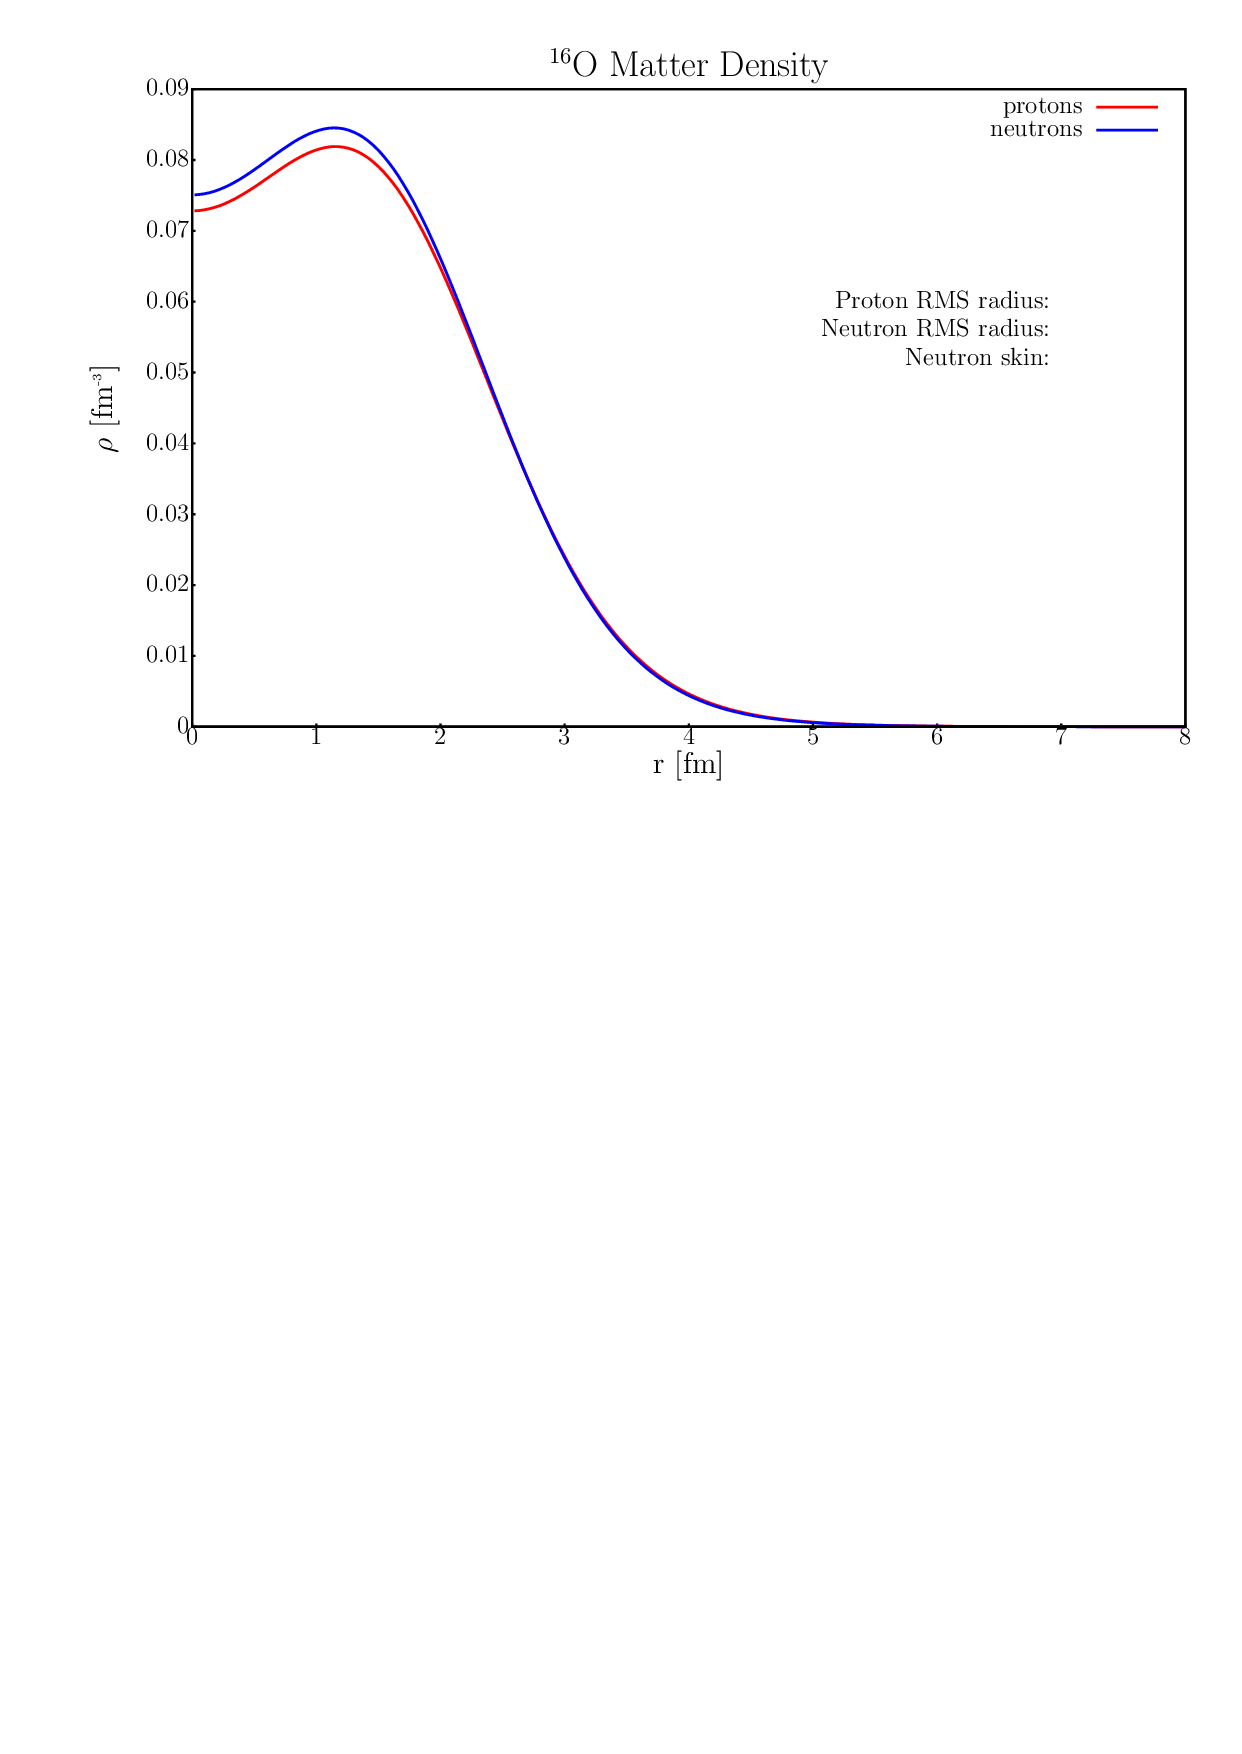
\includegraphics[width=\linewidth]{figures/o16_matterDensity.png}
        \caption{\oSix\ matter density distribution}
        \label{DOMFitData_o16_matterDensity}
    \end{subfigure}
\end{figure}

\newpage
\section{DOM fit of \oEight}
\label{o18DOMOutput}
\begin{figure}[hbtp]
    \captionsetup[subfigure]{labelformat=empty}
    \centering
    \begin{subfigure}[c]{0.39\textheight}
        \centering
        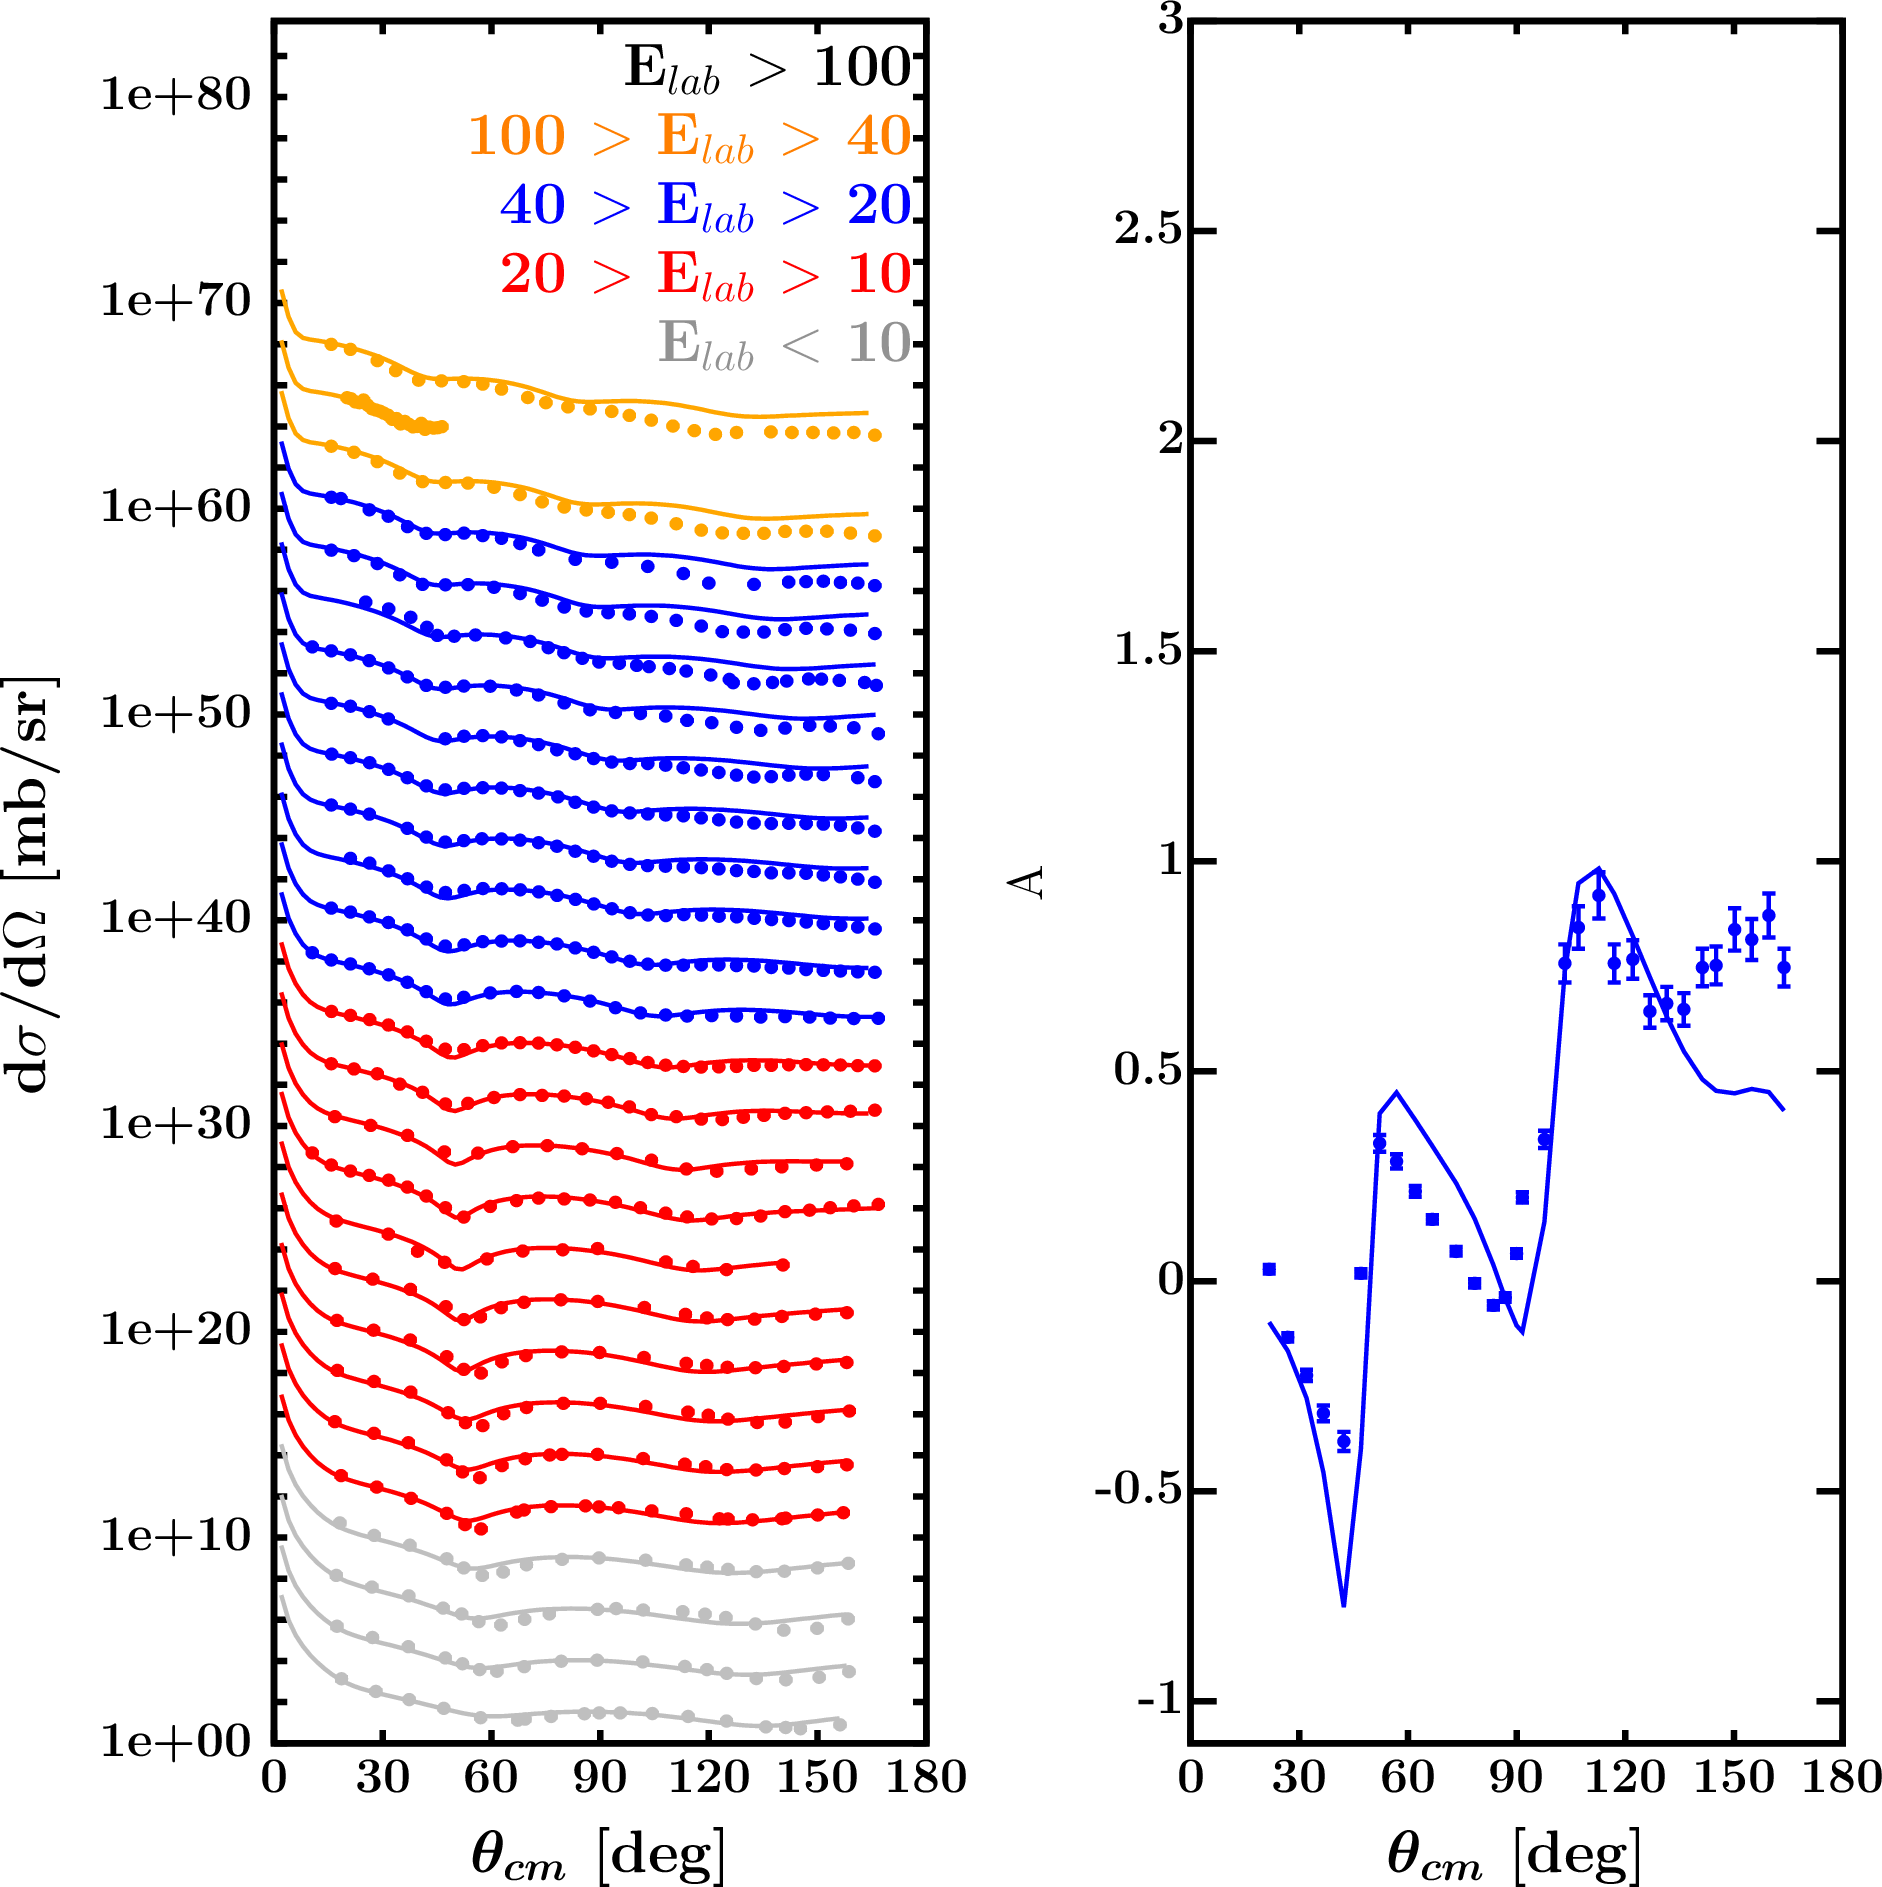
\includegraphics[width=\linewidth]{figures/o18_protonElastic.png}
        \caption{\oEight\ proton elastic scattering}
        \label{DOMFitData_o18_proton_elastic}
    \end{subfigure}\hspace{6pt}
    \begin{subfigure}[c]{0.39\textheight}
        \centering
        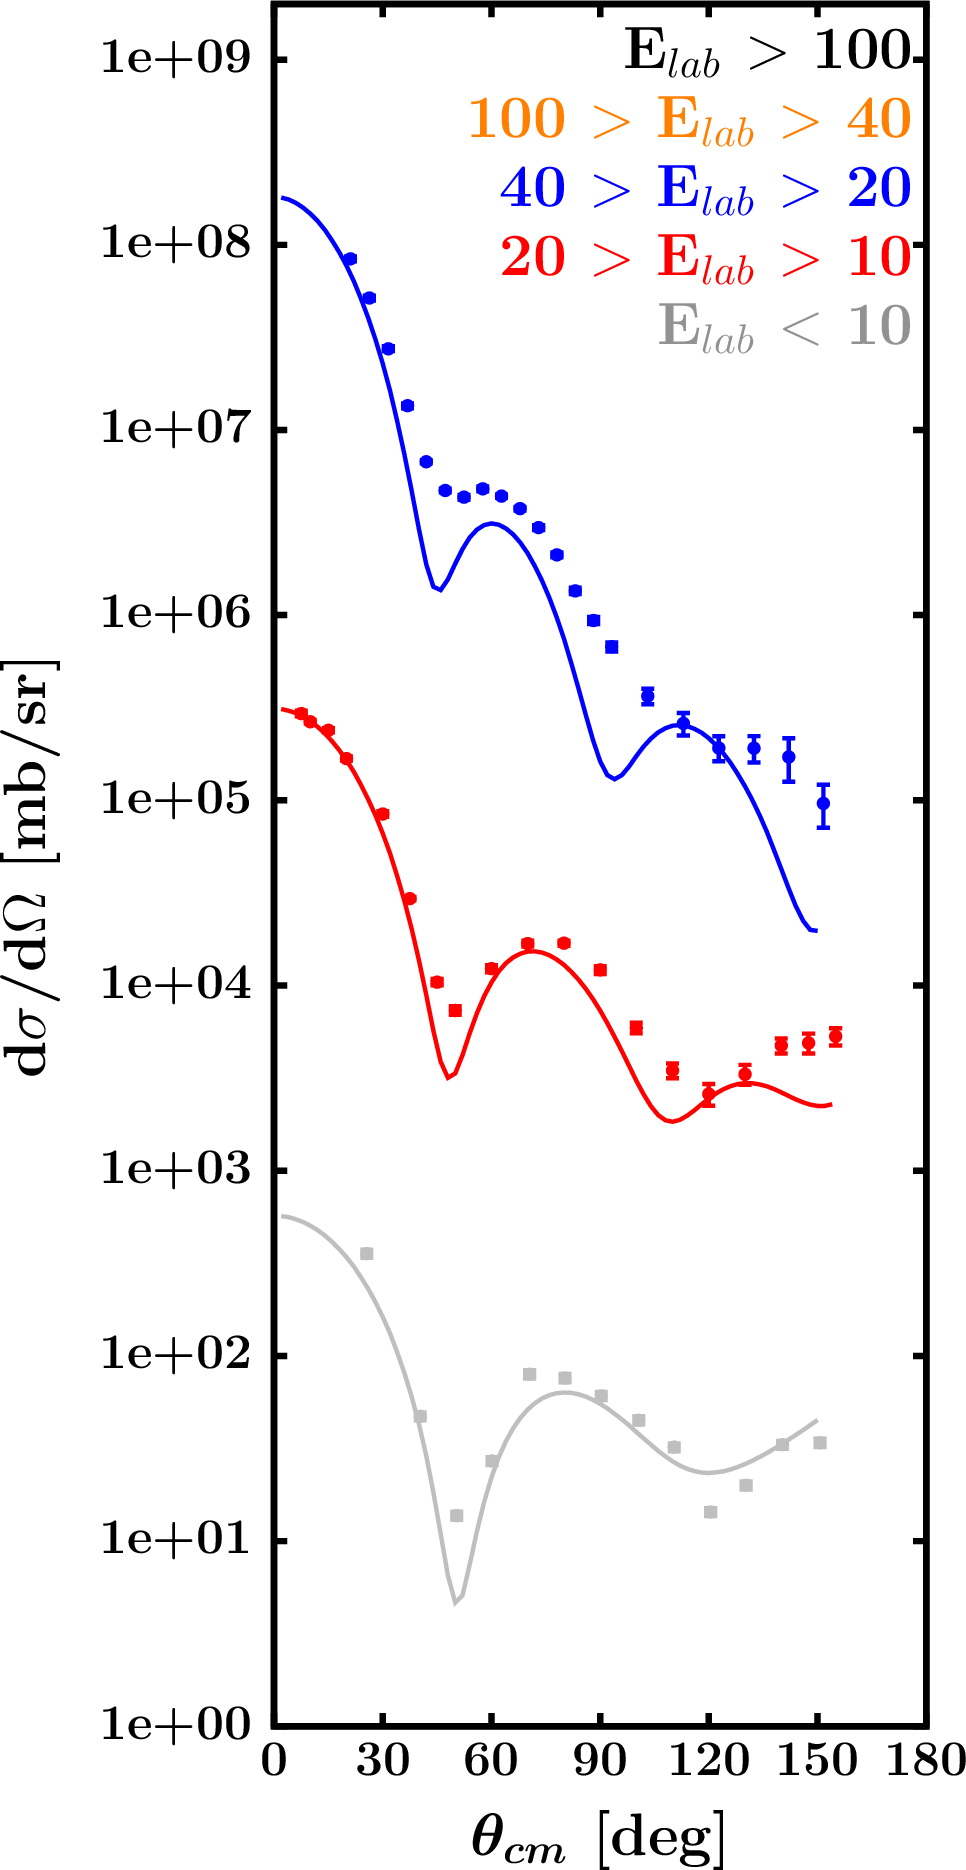
\includegraphics[width=0.52\linewidth]{figures/o18_neutronElastic.png}
        \caption{\oEight\ neutron elastic scattering}
        \label{DOMFitData_o18_neutron_elastic}
    \end{subfigure}\vspace{0.70in}
    \begin{subfigure}[c]{0.45\textwidth}
        \centering
        %
\includegraphics[width=\linewidth]{figures/o18_protonInelastic.png}
        \caption{No \oEight\ proton \rxn\\ data were available}
        \label{DOMFitData_o18_proton_inelastic}
    \end{subfigure}\hspace{6pt}
    \begin{subfigure}[c]{0.45\textwidth}
        \centering
        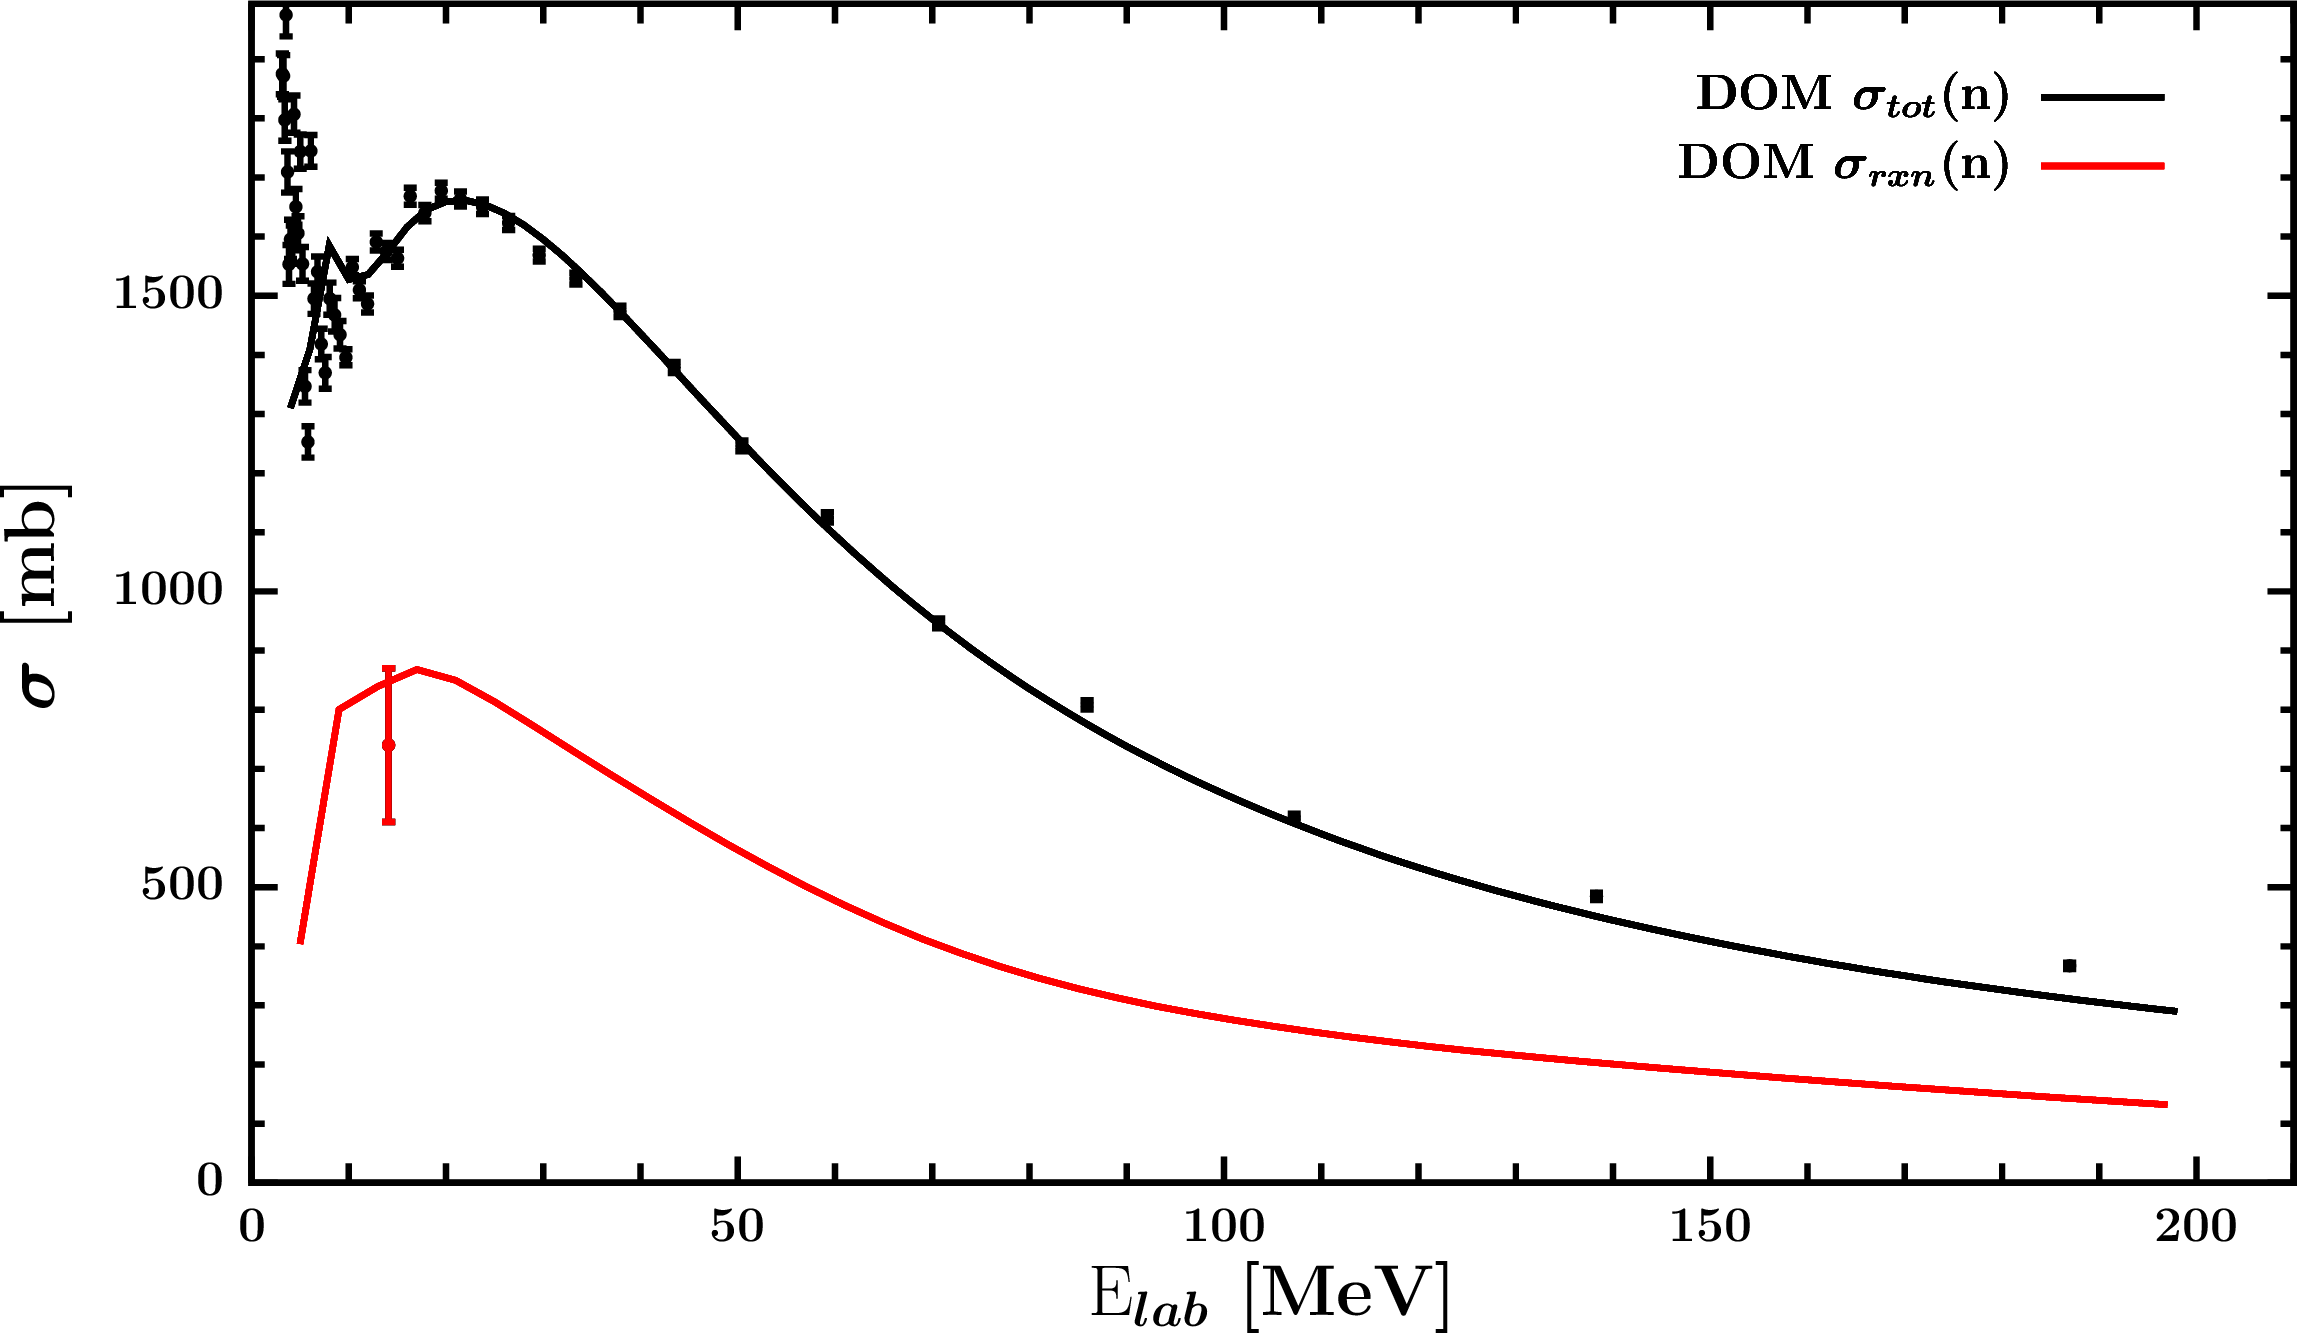
\includegraphics[width=\linewidth]{figures/o18_neutronInelastic.png}
        \caption{\oEight\ neutron \rxn\ and \tot}
        \label{DOMFitData_o18_neutron_inelastic}
    \end{subfigure}
\end{figure}
\afterpage{\clearpage}
\begin{figure}[hbtp]
    \captionsetup[subfigure]{labelformat=empty}
    \centering
    \begin{subfigure}[b]{0.45\textwidth}
        \centering
        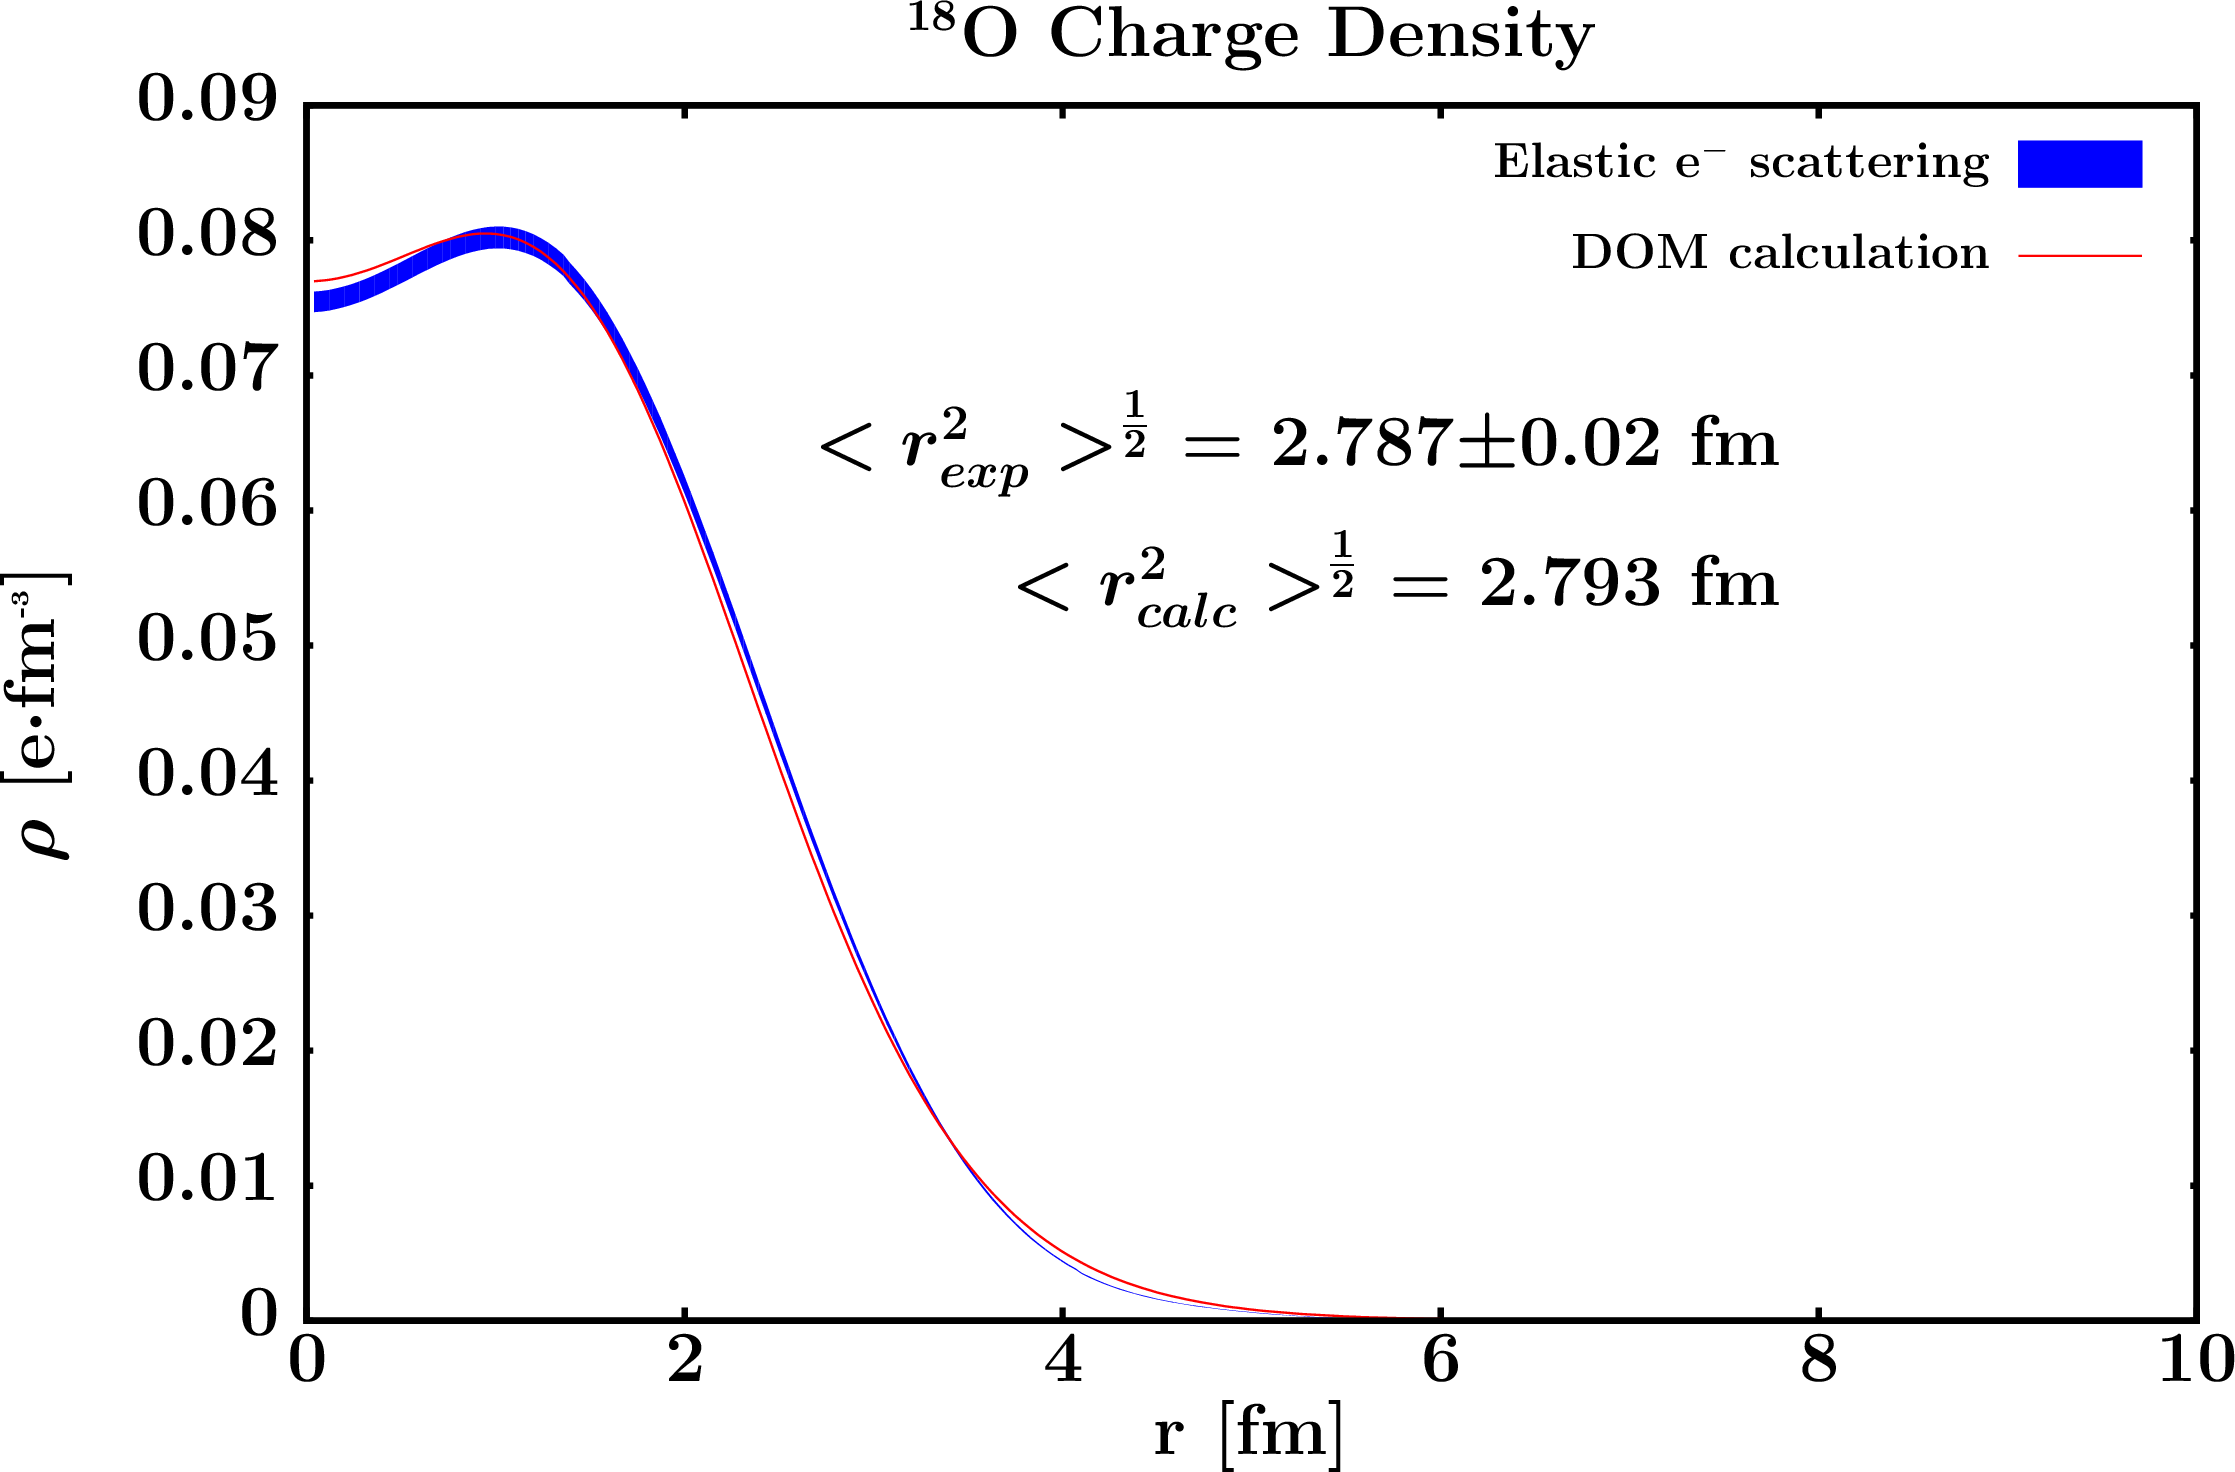
\includegraphics[width=\linewidth]{figures/o18_chargeDensity.png}
        \caption{\oEight\ charge density}
        \label{DOMFitData_o18_chargeDensity}
    \end{subfigure}\hspace{6pt}
    \begin{subfigure}[b]{0.45\textwidth}
        \centering
        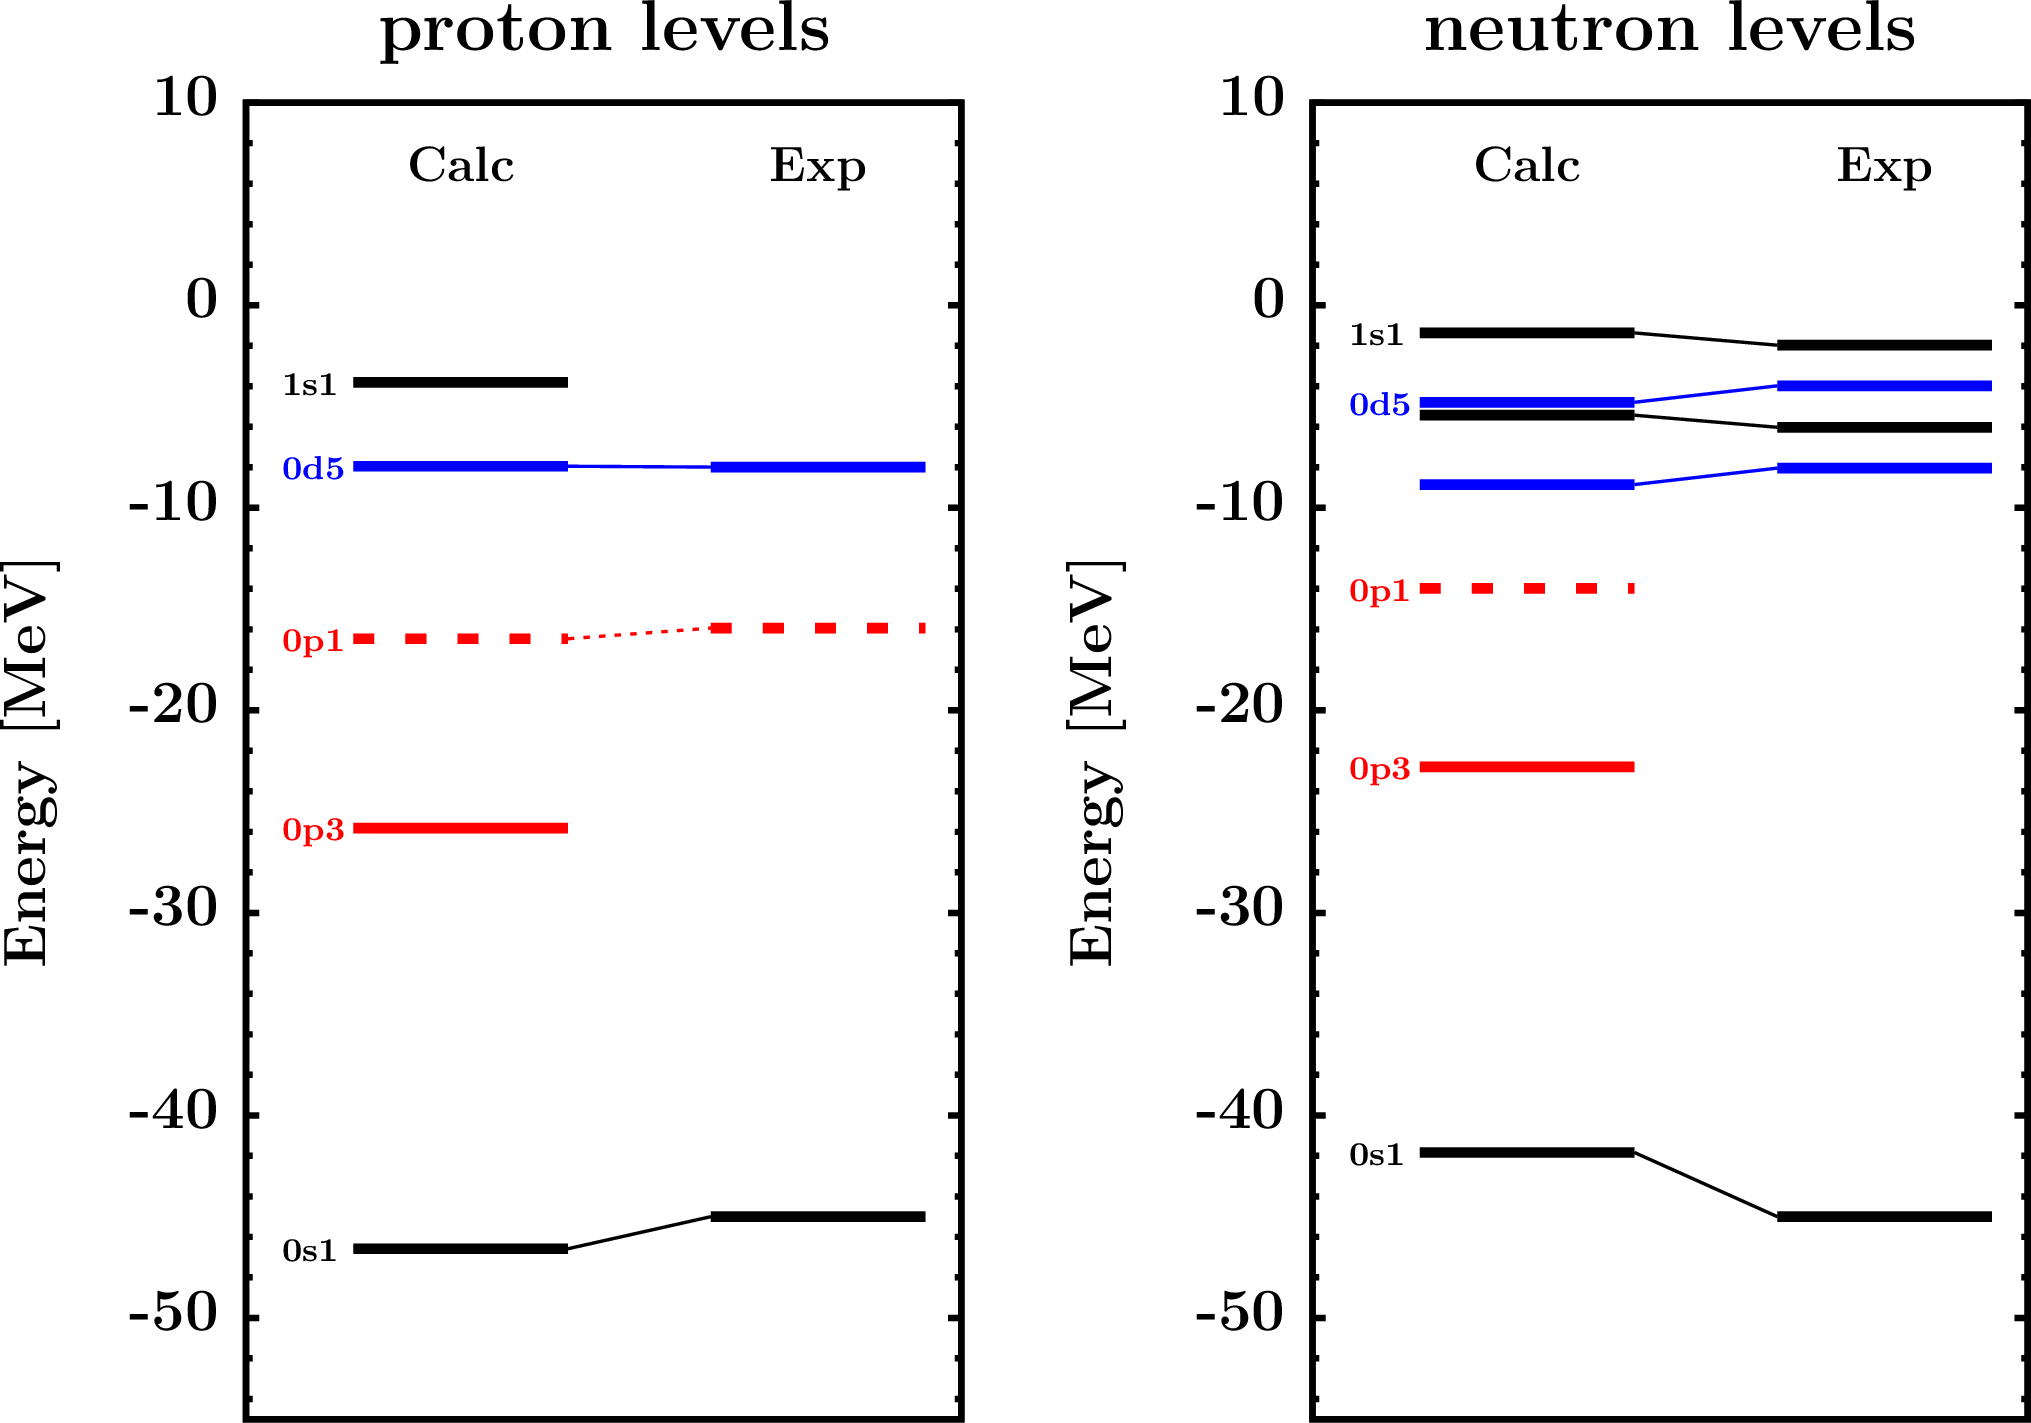
\includegraphics[width=\linewidth]{figures/o18_SPLevels.png}
        \caption{\oEight\ single-particle levels}
        \label{DOMFitData_o18_SPLevels}
    \end{subfigure}\vspace{0.3in}
    \begin{subfigure}[b]{0.45\textwidth}
        \centering
        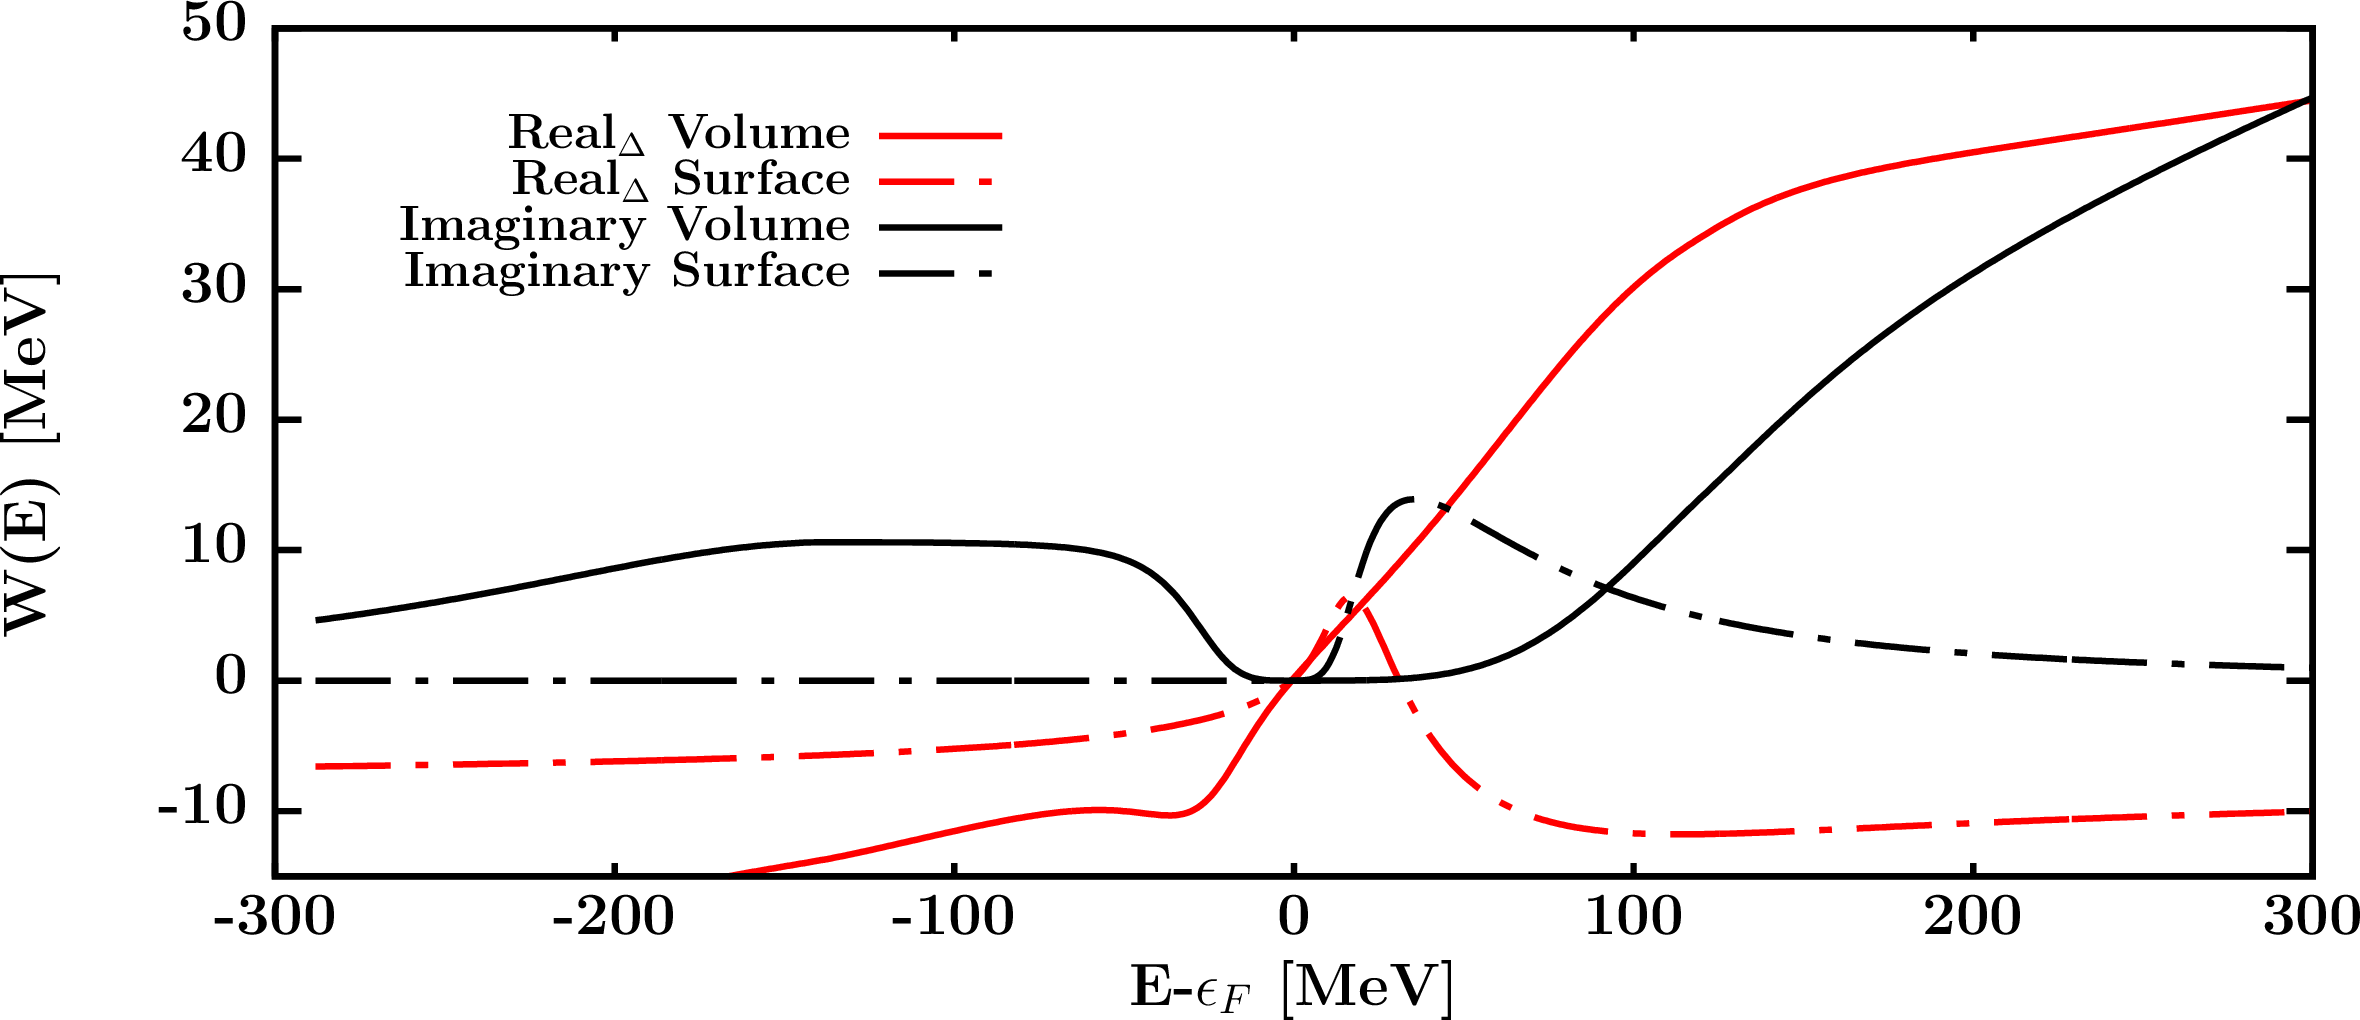
\includegraphics[width=\linewidth]{figures/o18_protonPotentials.png}
        \caption{\oEight\ proton potential energy-dependence}
        \label{DOMFitData_o18_proton_potentialComponent_energy}
    \end{subfigure}\hspace{6pt}
    \begin{subfigure}[b]{0.45\linewidth}
        \centering
        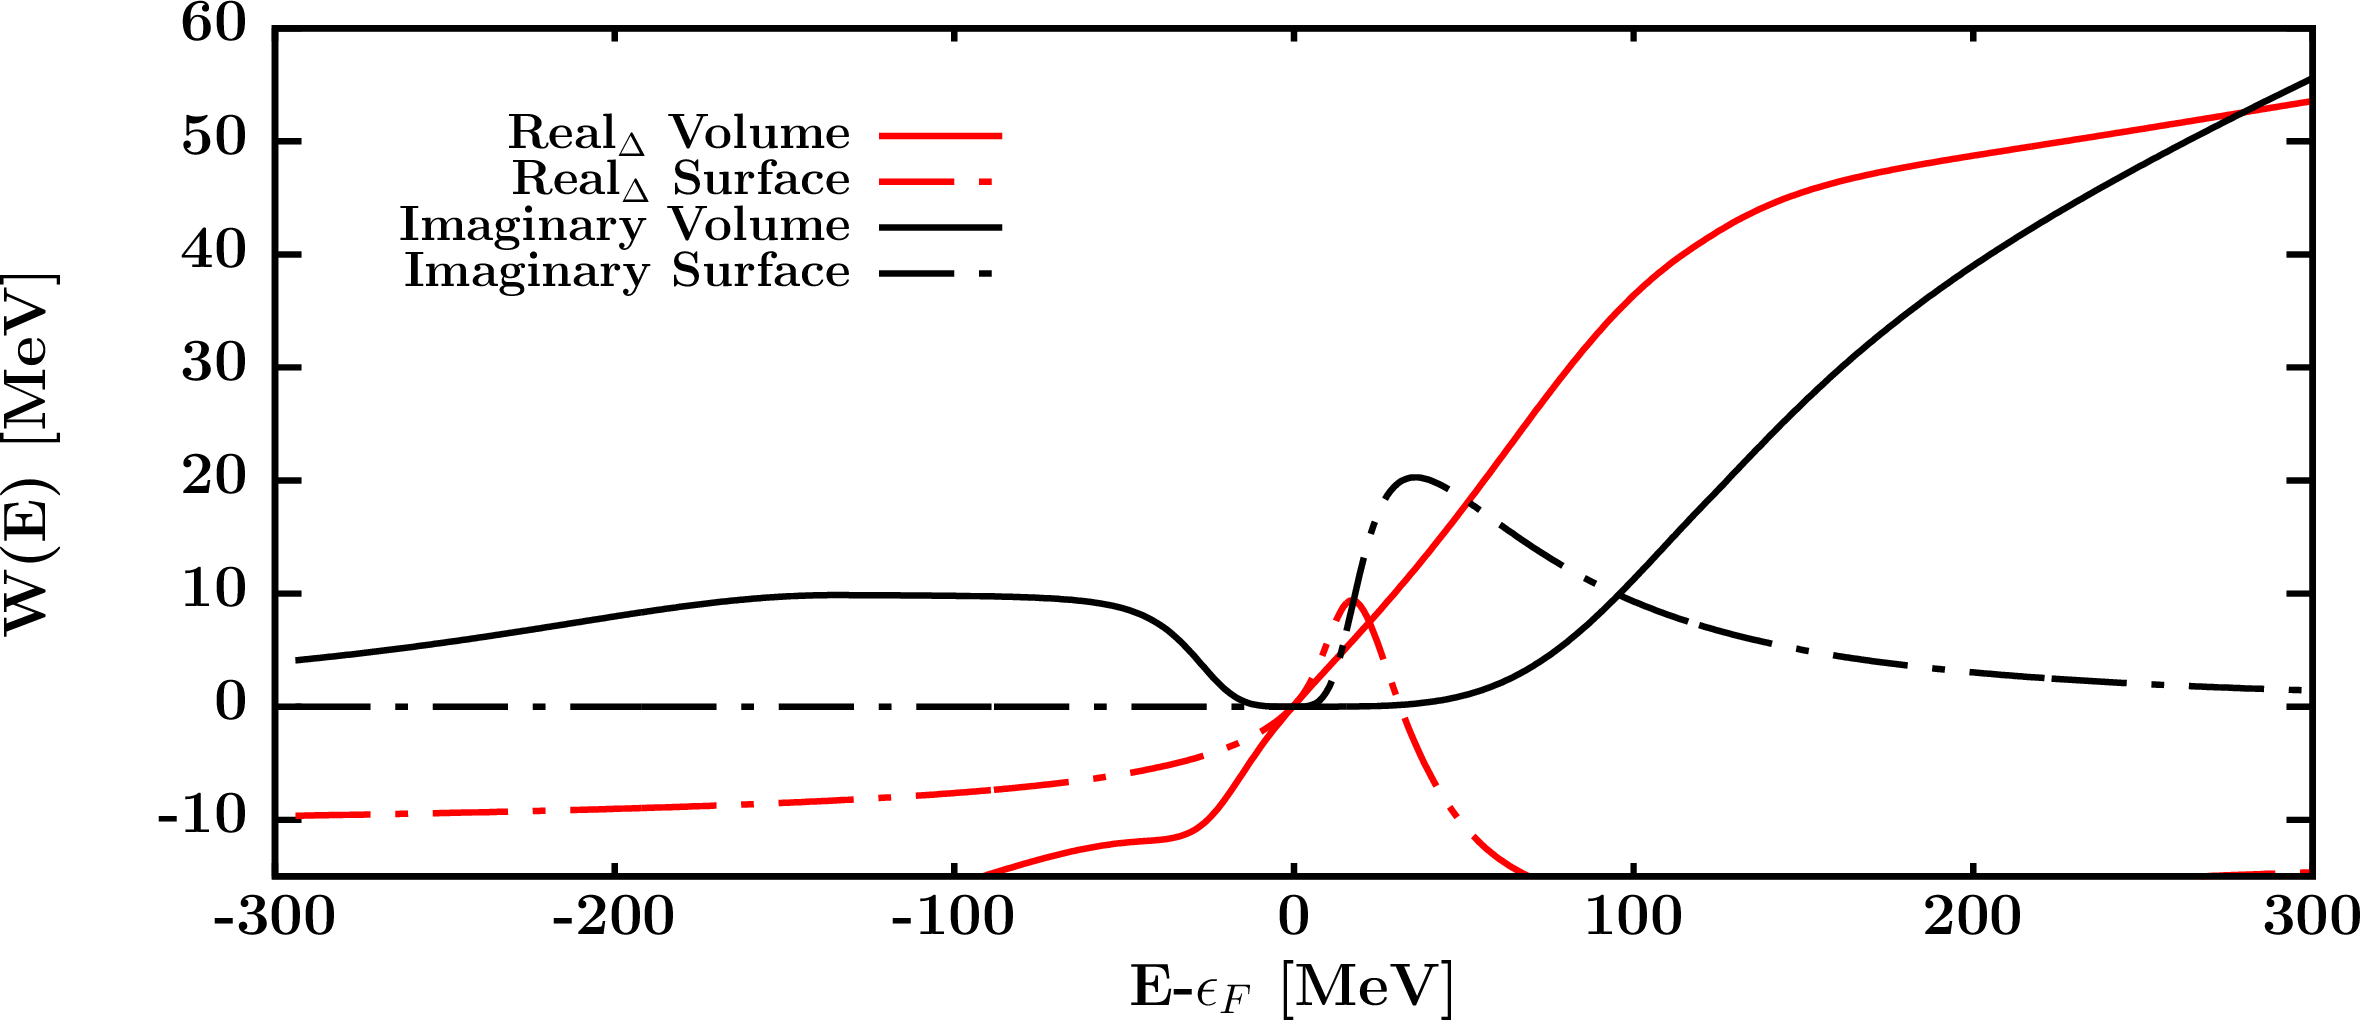
\includegraphics[width=\linewidth]{figures/o18_neutronPotentials.png}
        \caption{\oEight\ neutron potential energy-dependence}
        \label{DOMFitData_o18_neutron_potentialComponent_energy}
    \end{subfigure}\vspace{0.3in}
    \begin{subfigure}[b]{0.45\textwidth}
        \centering
        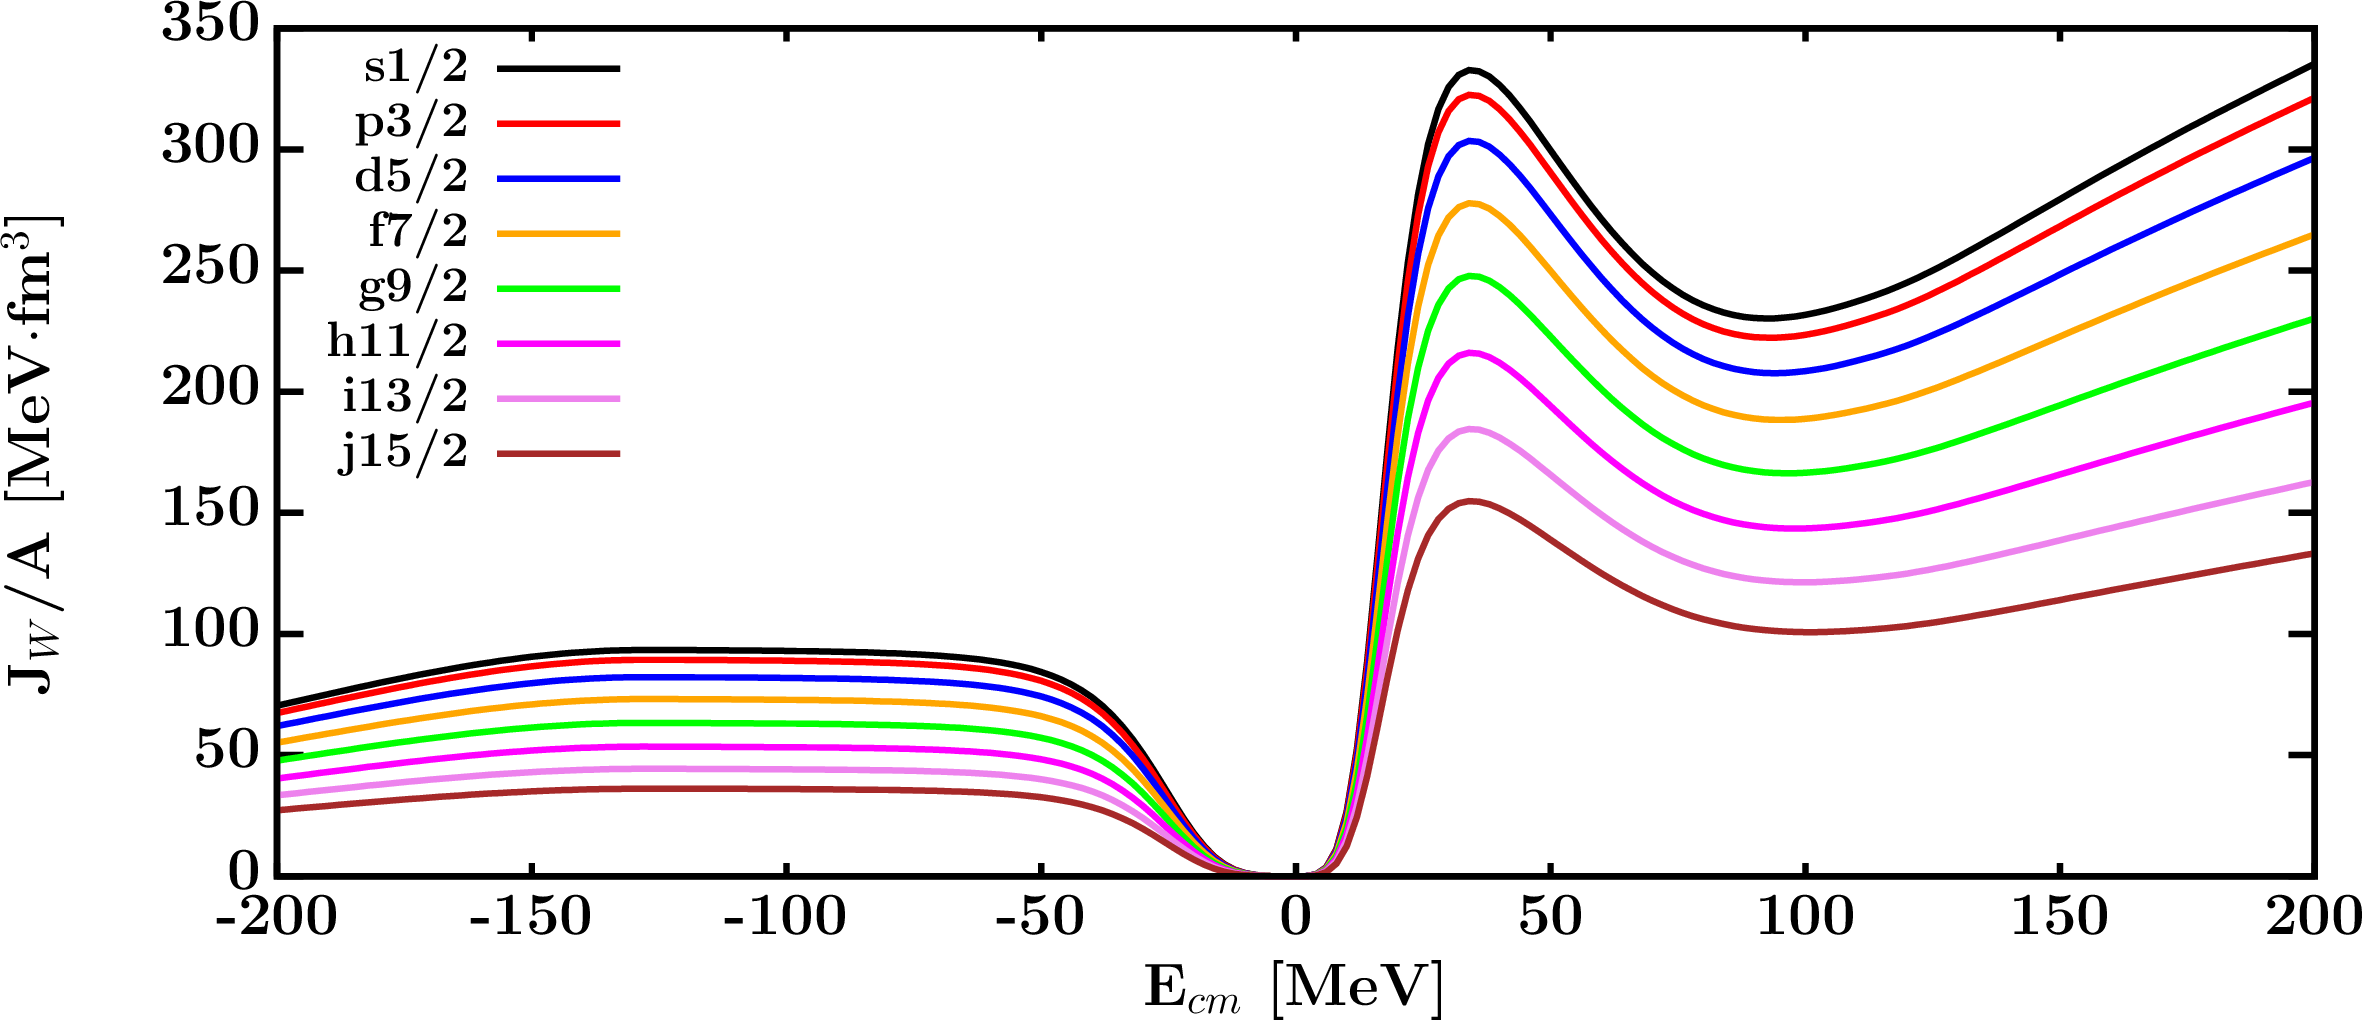
\includegraphics[width=\linewidth]{figures/o18_protonVolumeIntegrals.png}
        \caption{\oEight\ proton volume integral}
        \label{DOMFitData_o18_proton_potentialIntegral}
    \end{subfigure}\hspace{6pt}
    \begin{subfigure}[b]{0.45\textwidth}
        \centering
        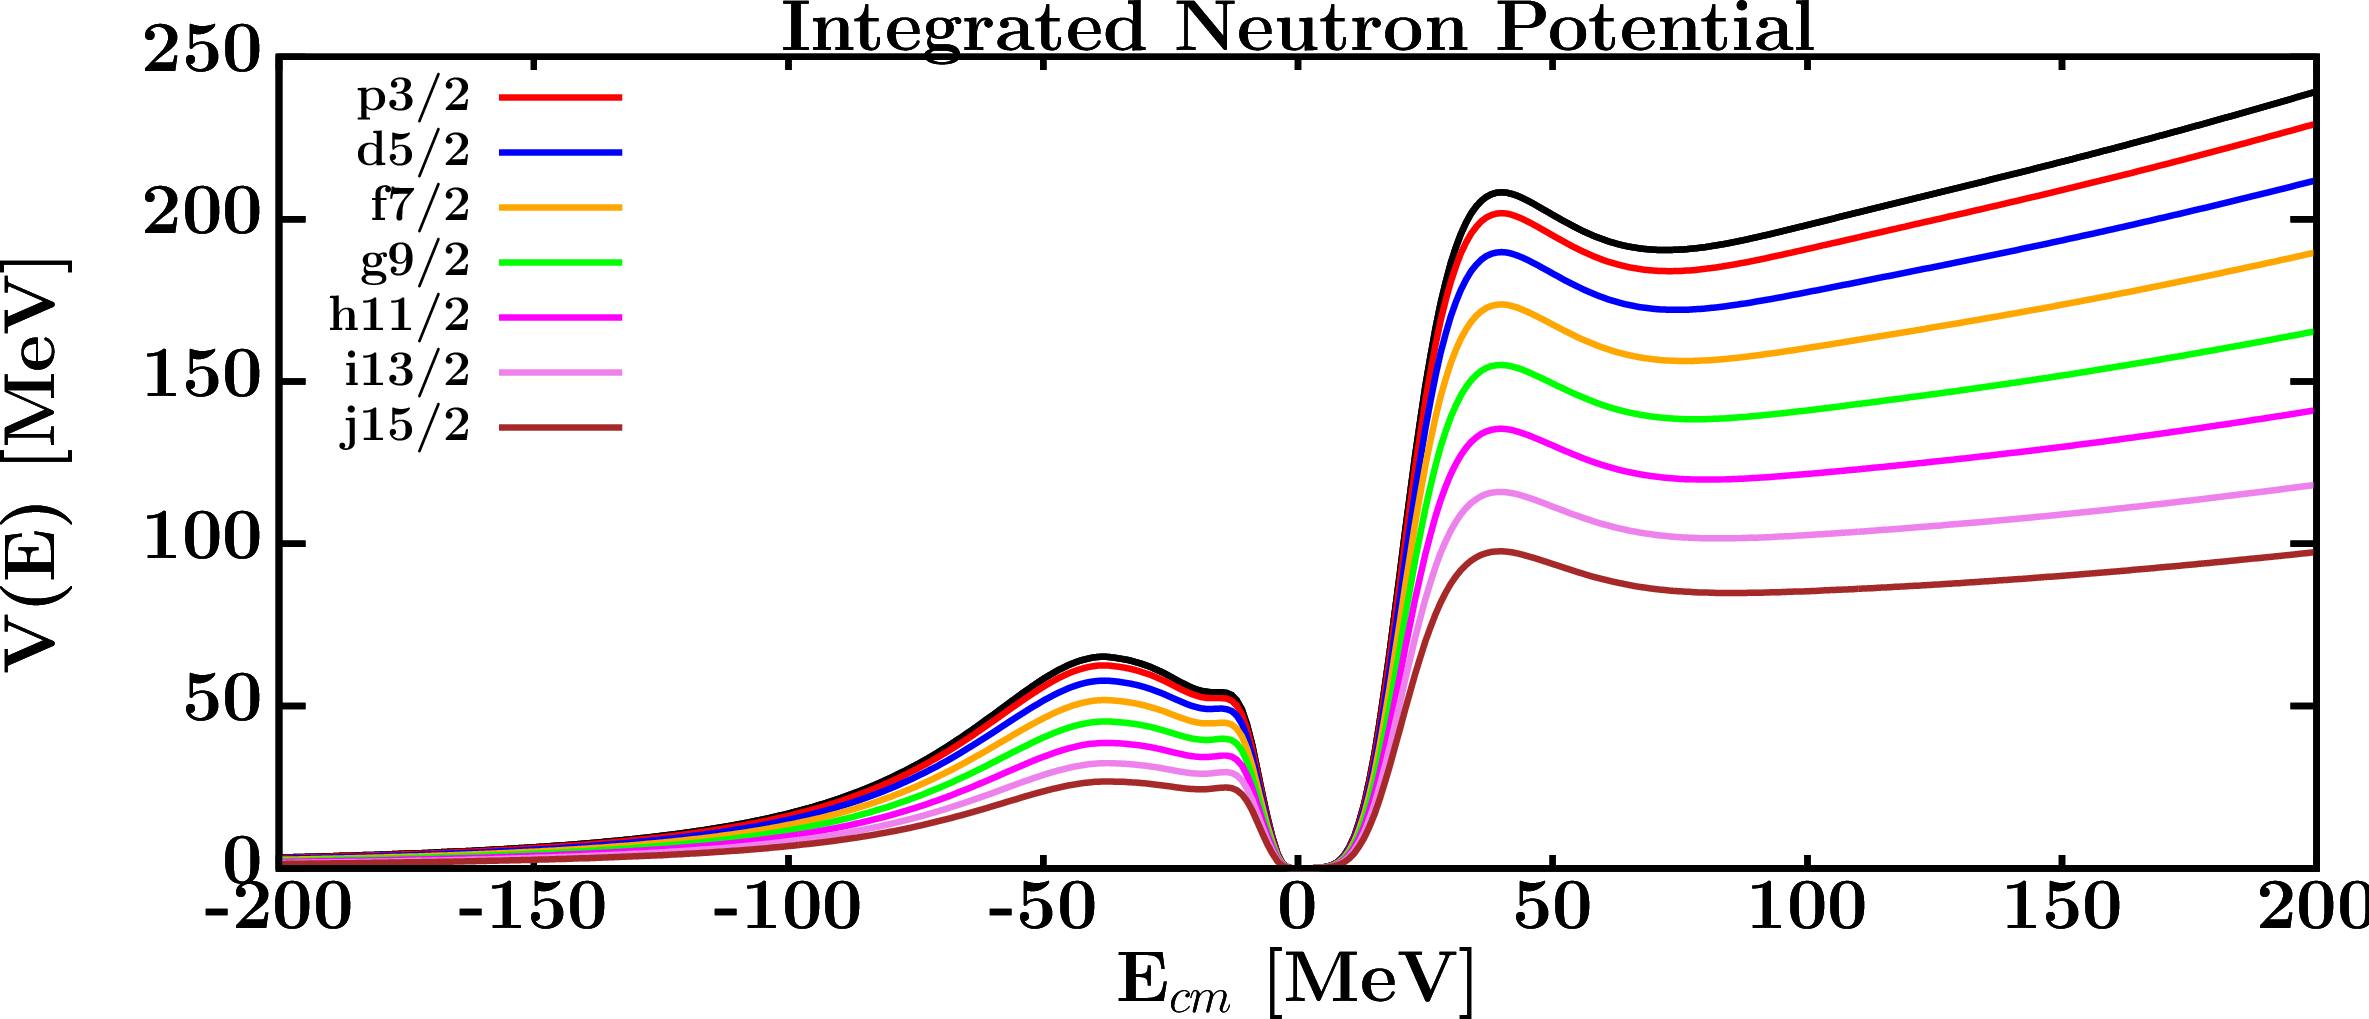
\includegraphics[width=\linewidth]{figures/o18_neutronVolumeIntegrals.png}
        \caption{\oEight\ neutron volume integral}
        \label{DOMFitData_o18_neutron_potentialIntegral}
    \end{subfigure}\vspace{0.3in}
    \begin{subfigure}[b]{0.45\textwidth}
        \centering
        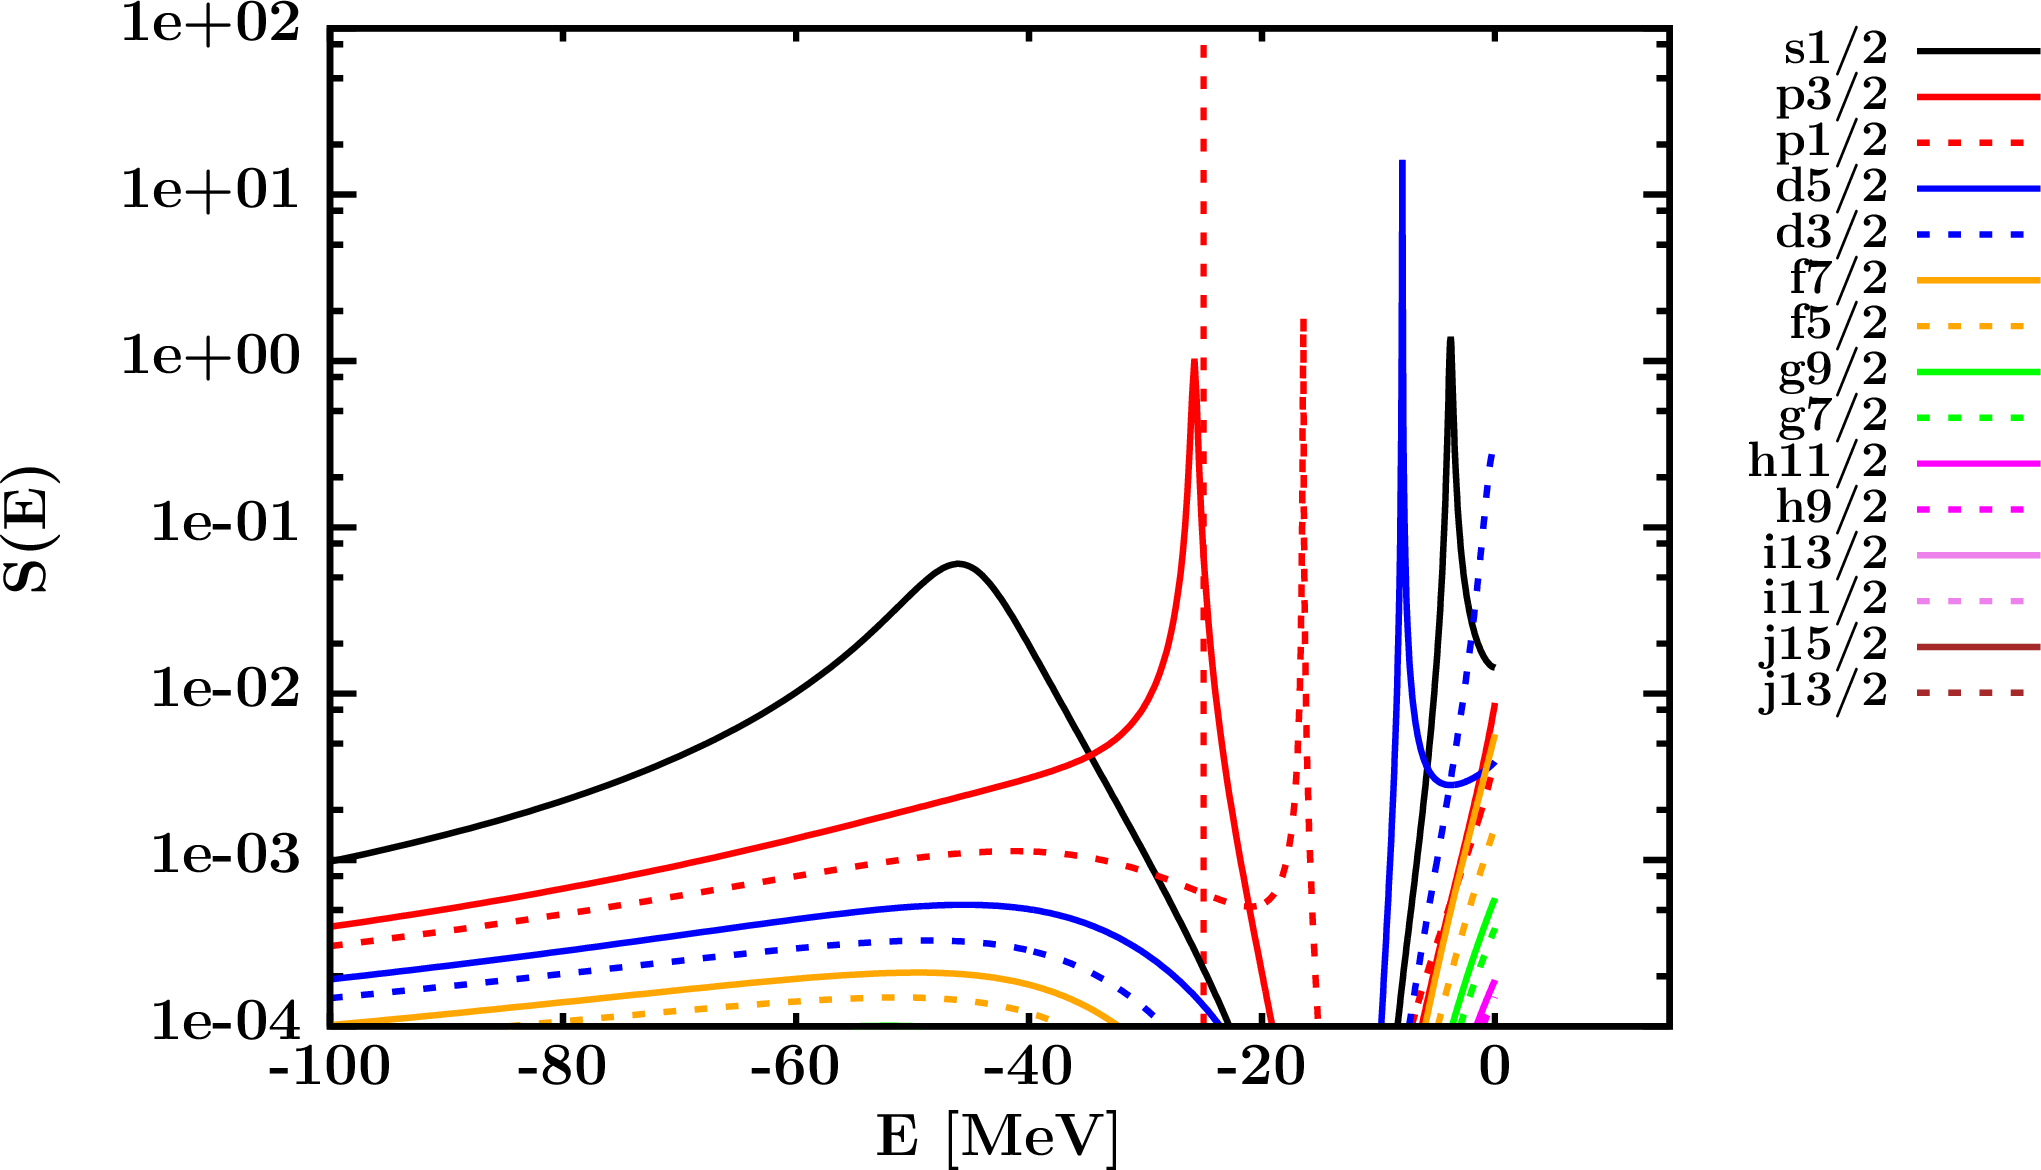
\includegraphics[width=\linewidth]{figures/o18_protonSpectralFunctions.png}
        \caption{\oEight\ proton spectral functions}
        \label{DOMFitData_o18_proton_spectralFunctions}
    \end{subfigure}\hspace{6pt}
    \begin{subfigure}[b]{0.45\textwidth}
        \centering
        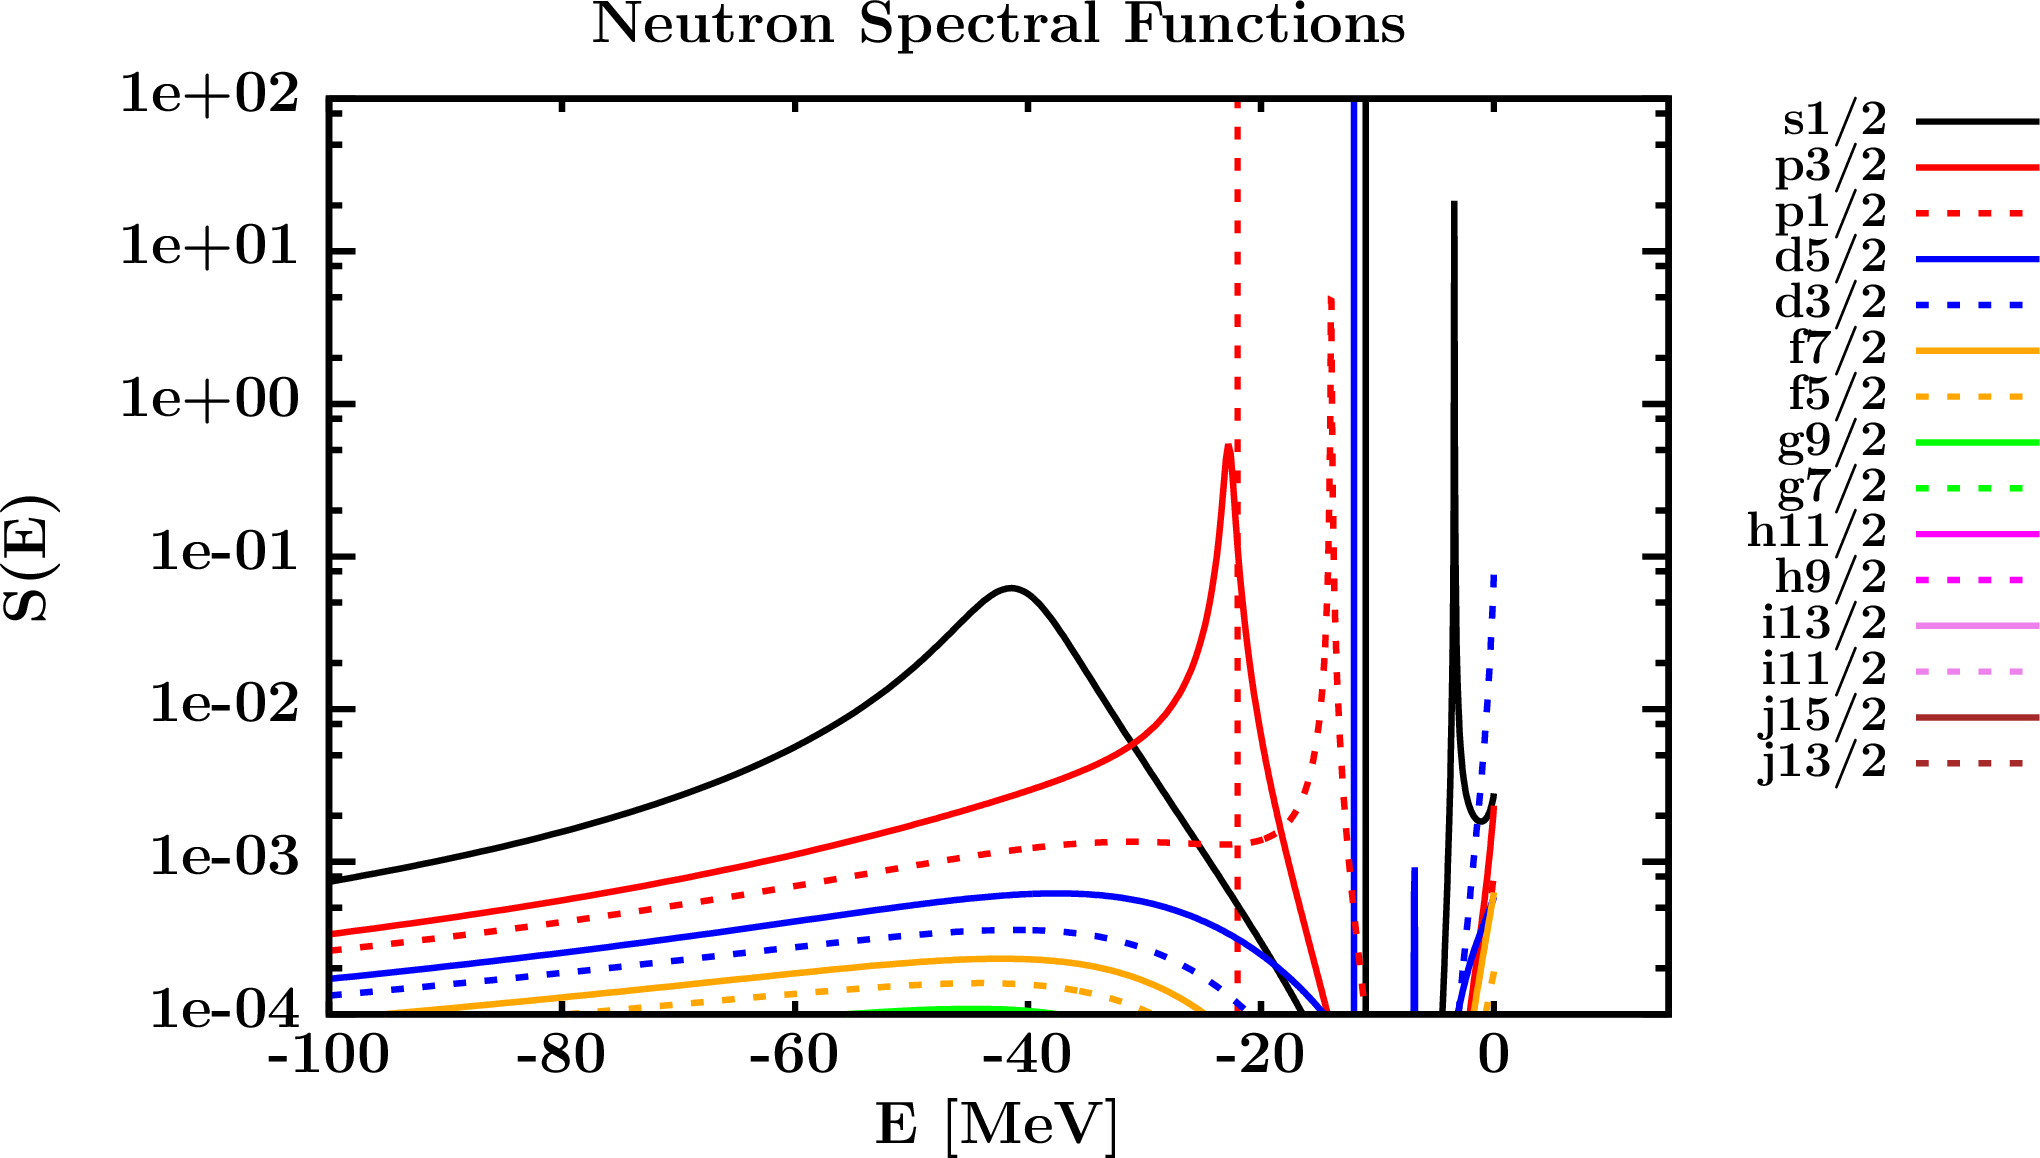
\includegraphics[width=\linewidth]{figures/o18_neutronSpectralFunctions.png}
        \caption{\oEight\ neutron spectral functions}
        \label{DOMFitData_o18_neutron_spectralFunctions}
    \end{subfigure}
\end{figure}
\afterpage{\clearpage}
\begin{figure}[hbtp]
    \captionsetup[subfigure]{labelformat=empty}
    \centering
    \begin{subfigure}[b]{0.45\textwidth}
        \centering
        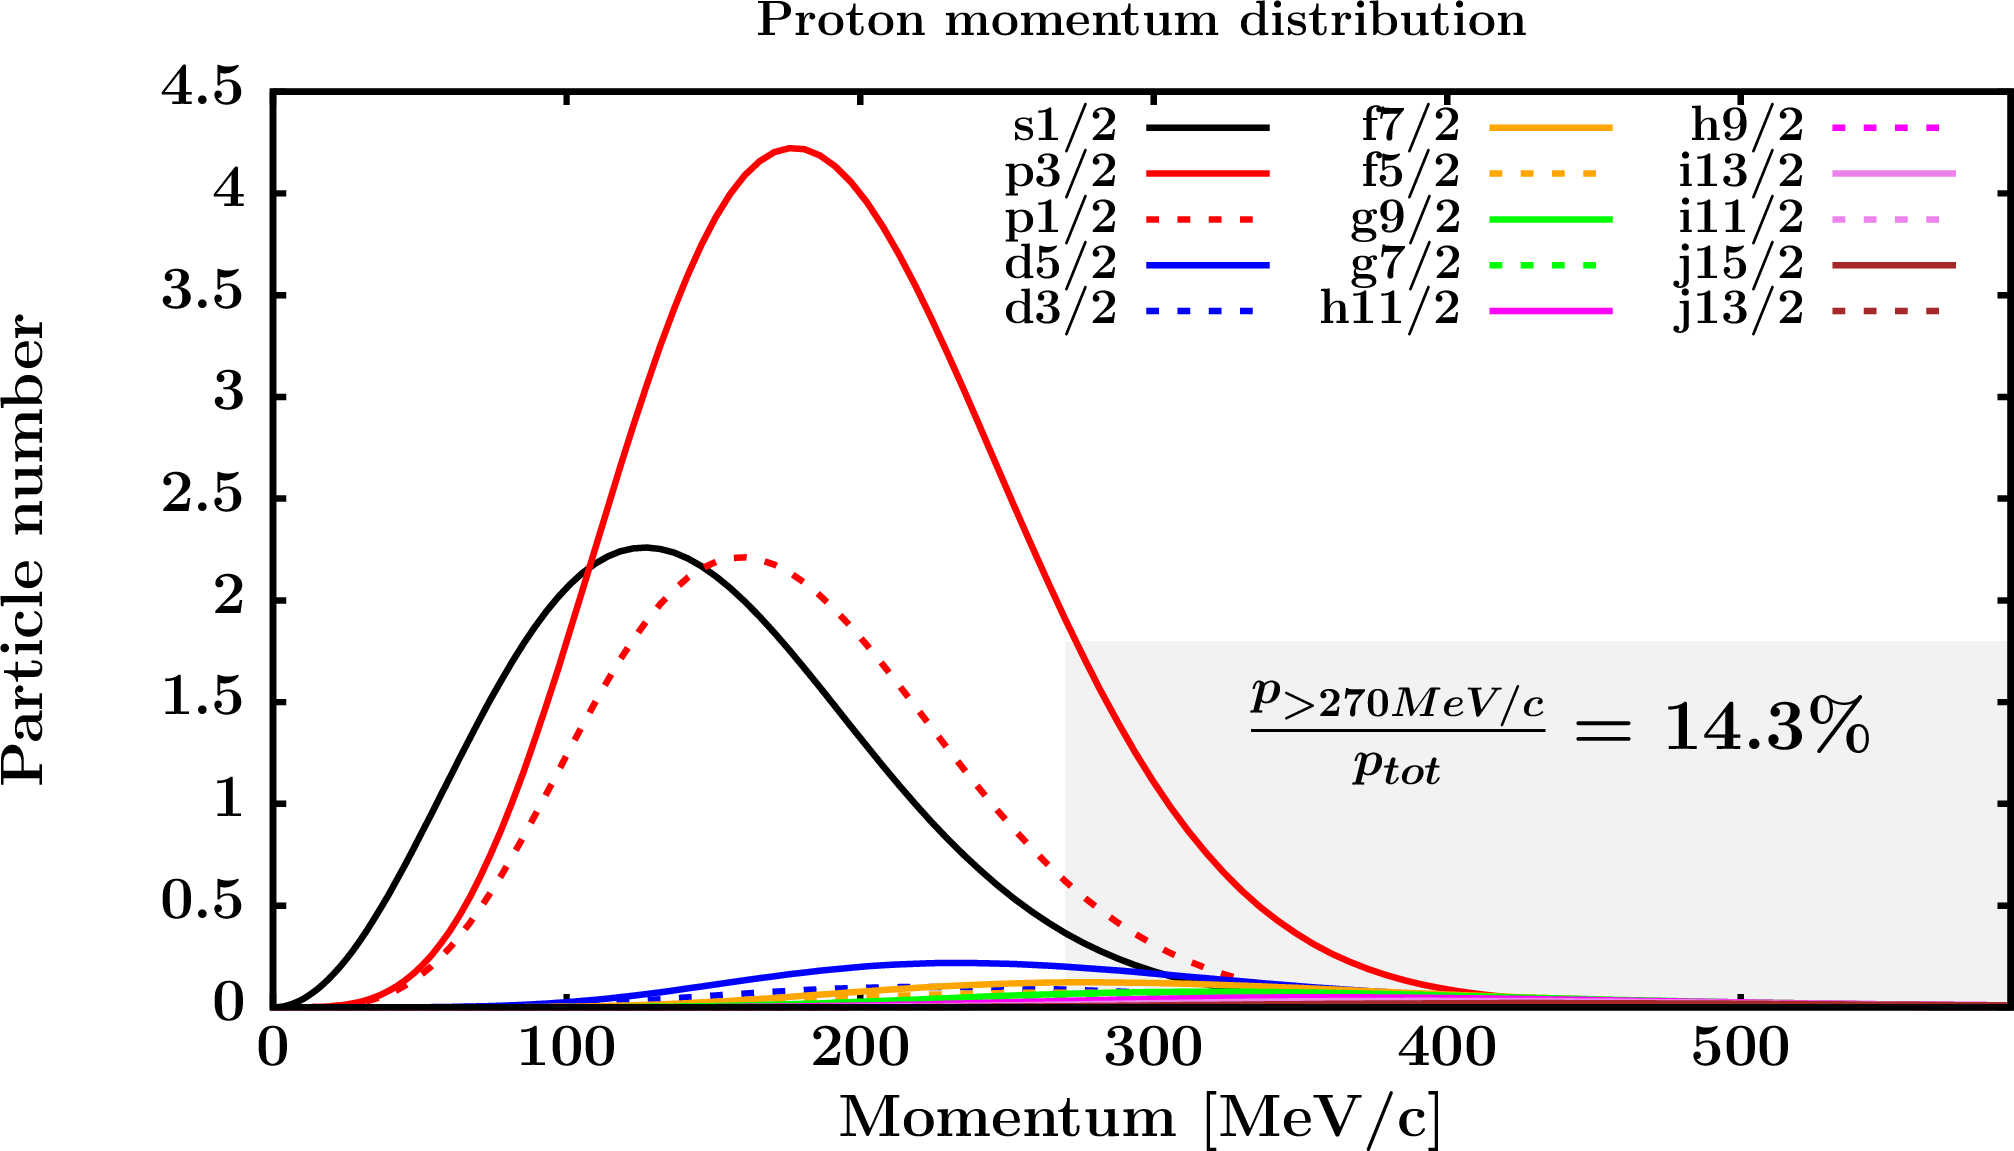
\includegraphics[width=\linewidth]{figures/o18_protonLJMomentumDistIntegral.png}
        \caption{\oEight\ proton momentum distribution}
        \label{DOMFitData_o18_proton_momentumDist}
    \end{subfigure}\hspace{6pt}
    \begin{subfigure}[b]{0.45\textwidth}
        \centering
        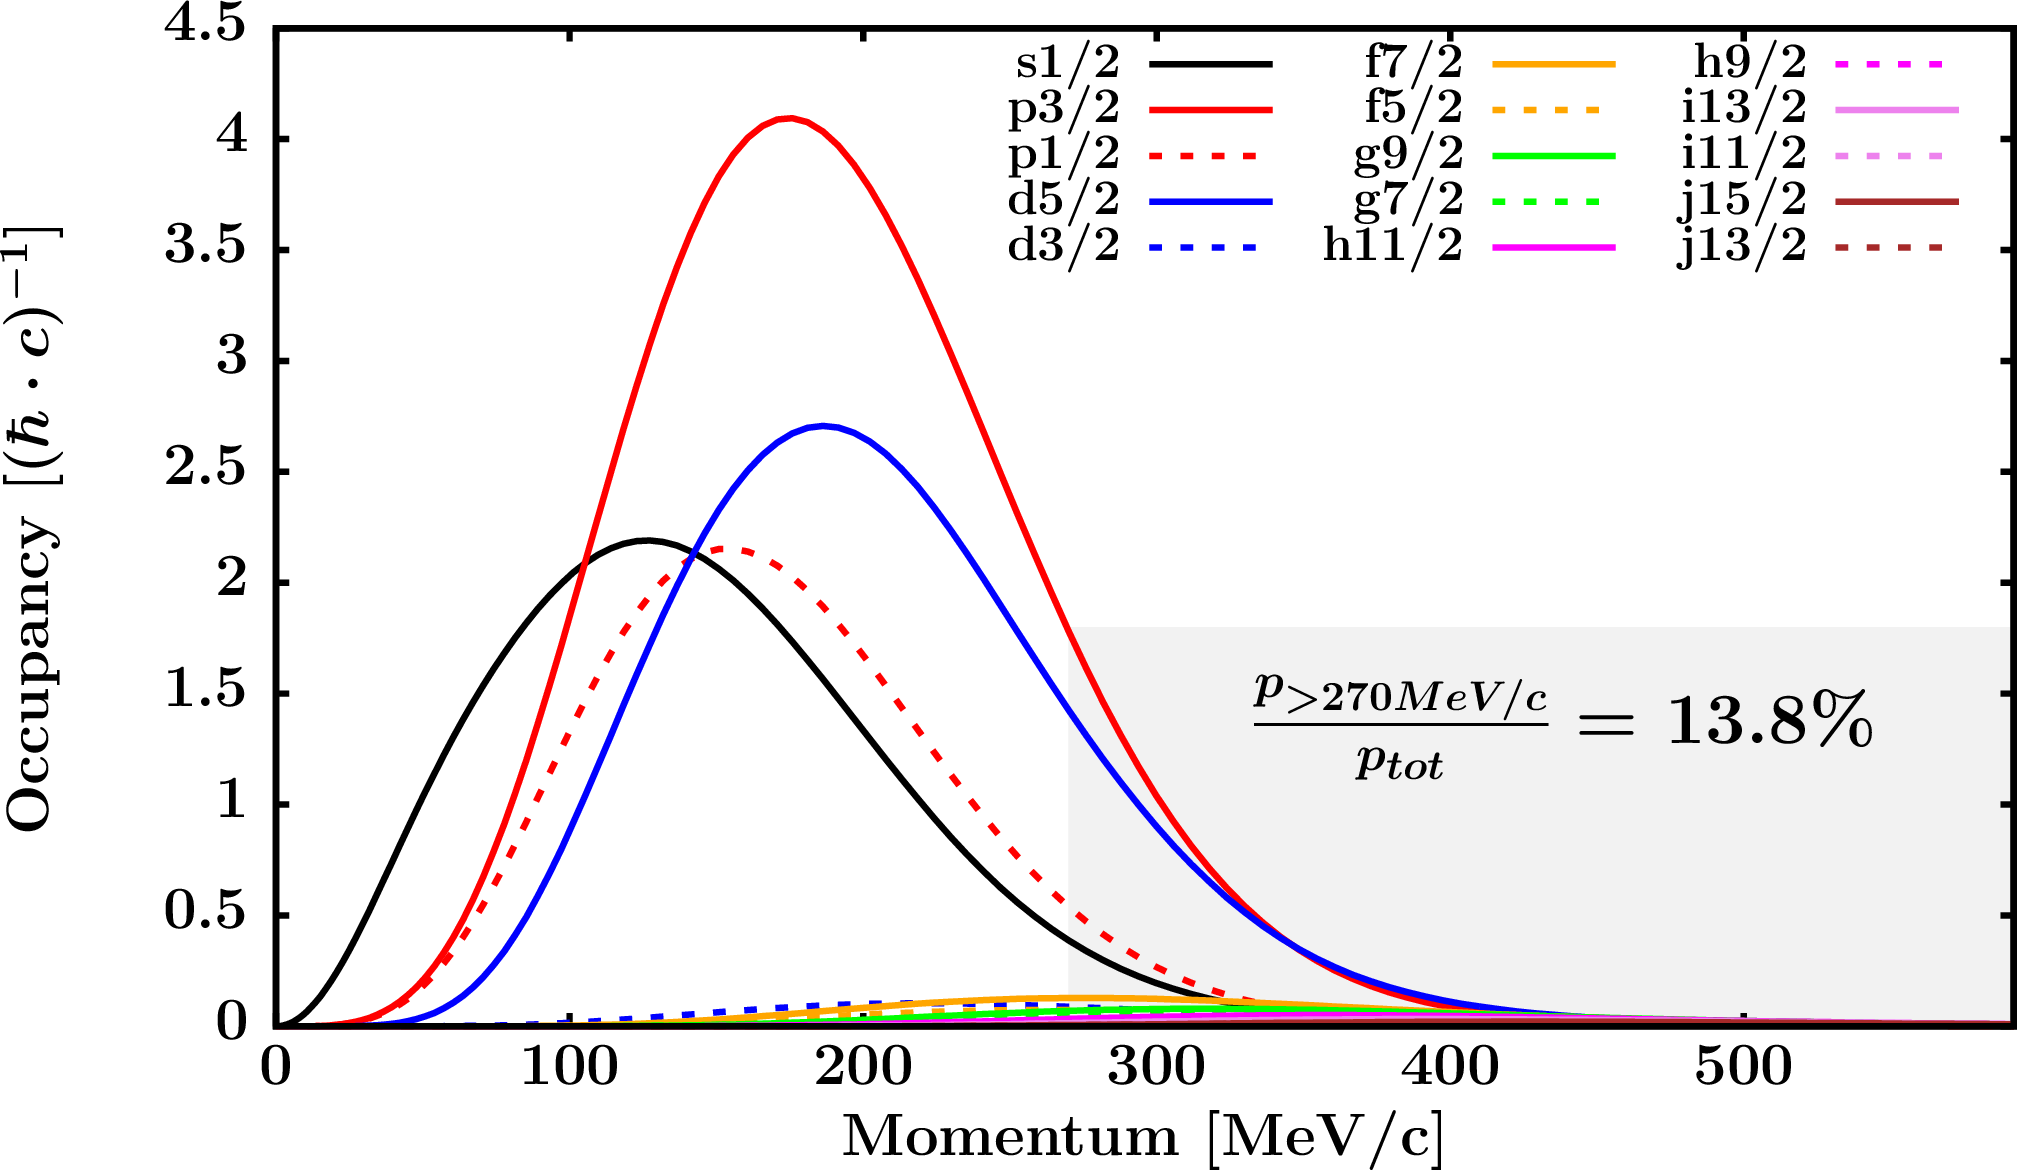
\includegraphics[width=\linewidth]{figures/o18_neutronLJMomentumDistIntegral.png}
        \caption{\oEight\ neutron momentum distribution}
        \label{DOMFitData_o18_neutron_momentumDist}
    \end{subfigure}\vspace{0.3in}
    \begin{subfigure}{0.45\textwidth}
        \centering
        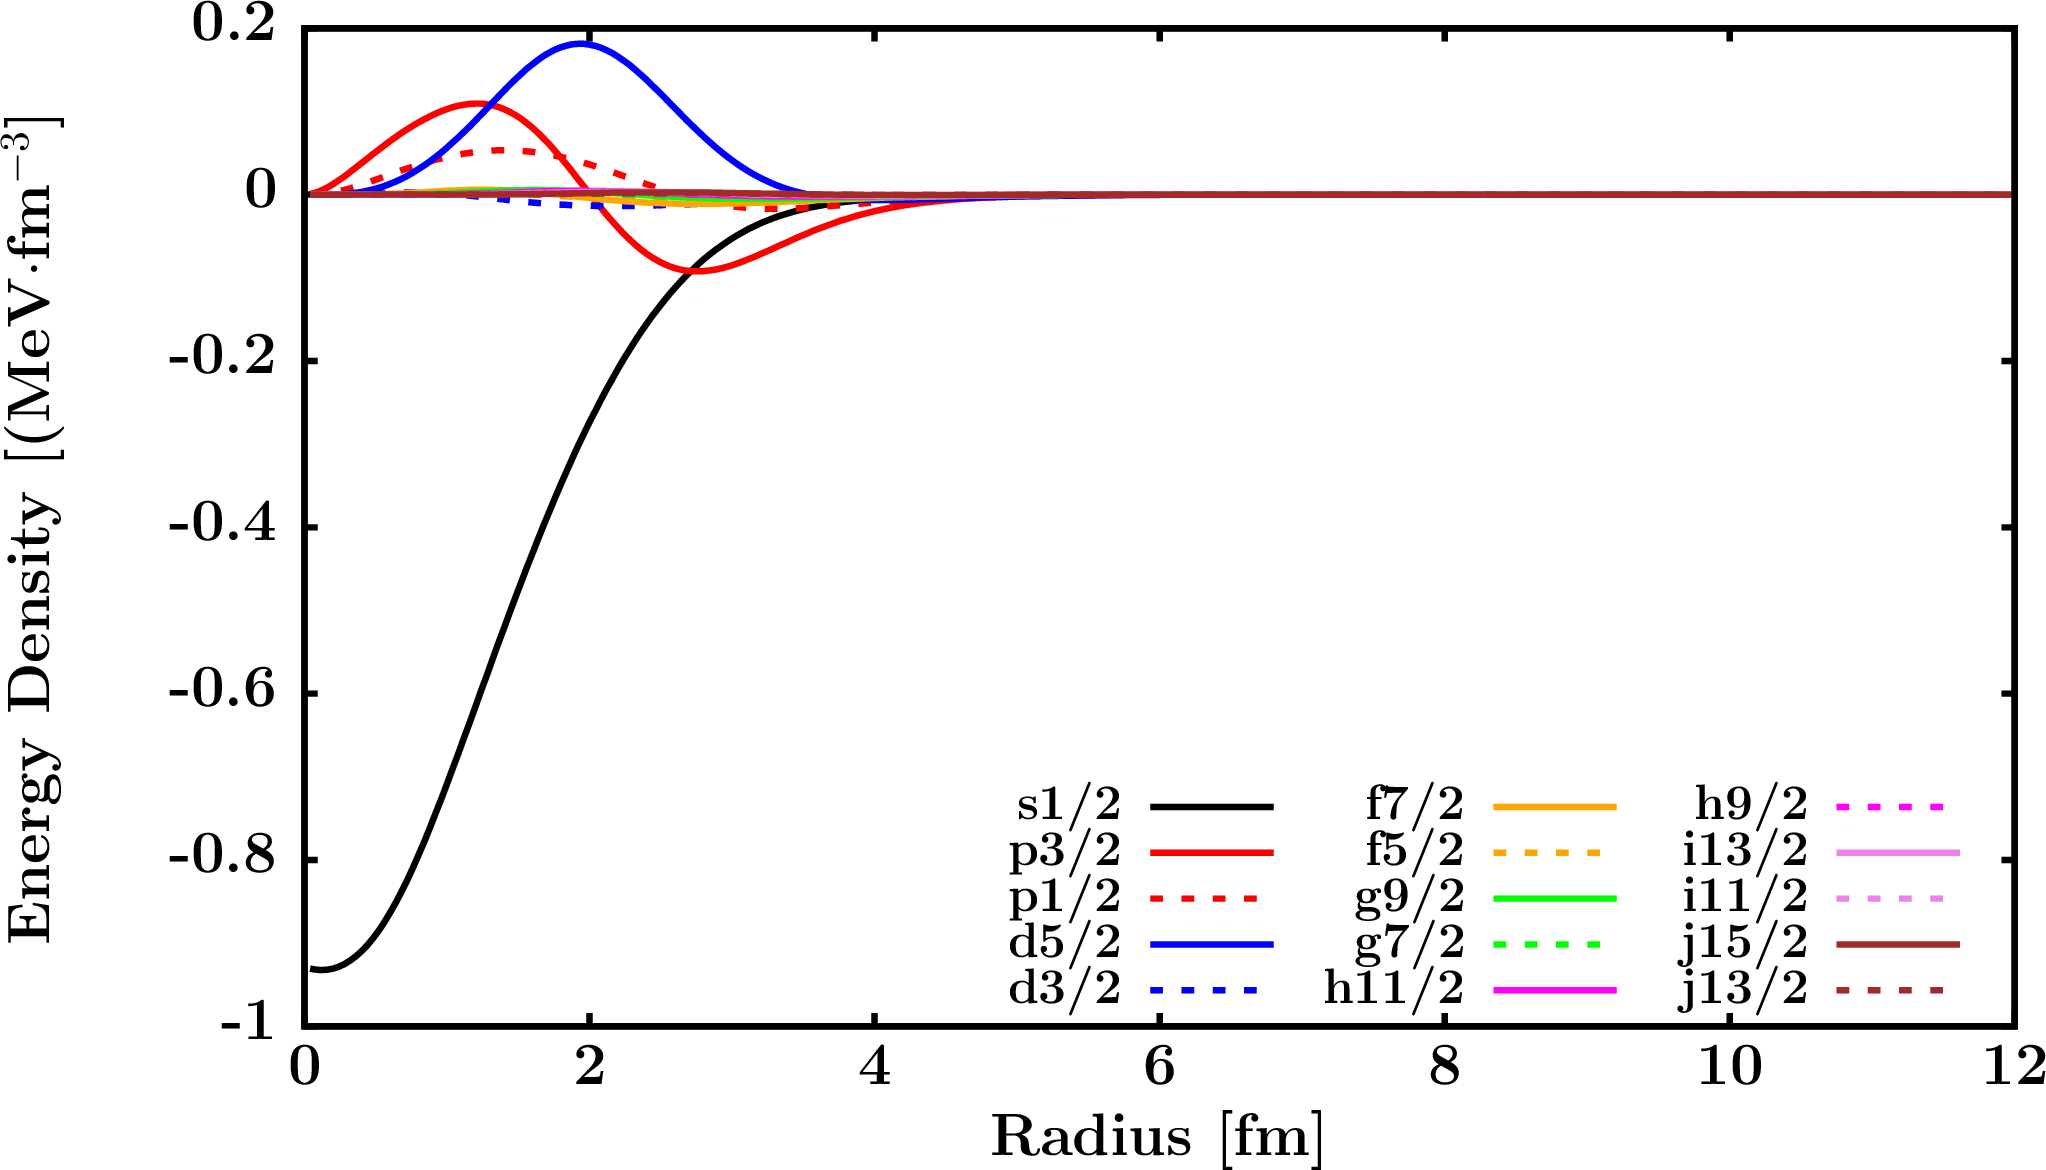
\includegraphics[width=\linewidth]{figures/o18_EnergyDist.png}
        \caption{\oEight\ energy distribution by LJ}
        \label{DOMFitData_o18_proton_energyDistInt}
    \end{subfigure}\hspace{6pt}
    \begin{subfigure}{0.45\textwidth}
        \centering
        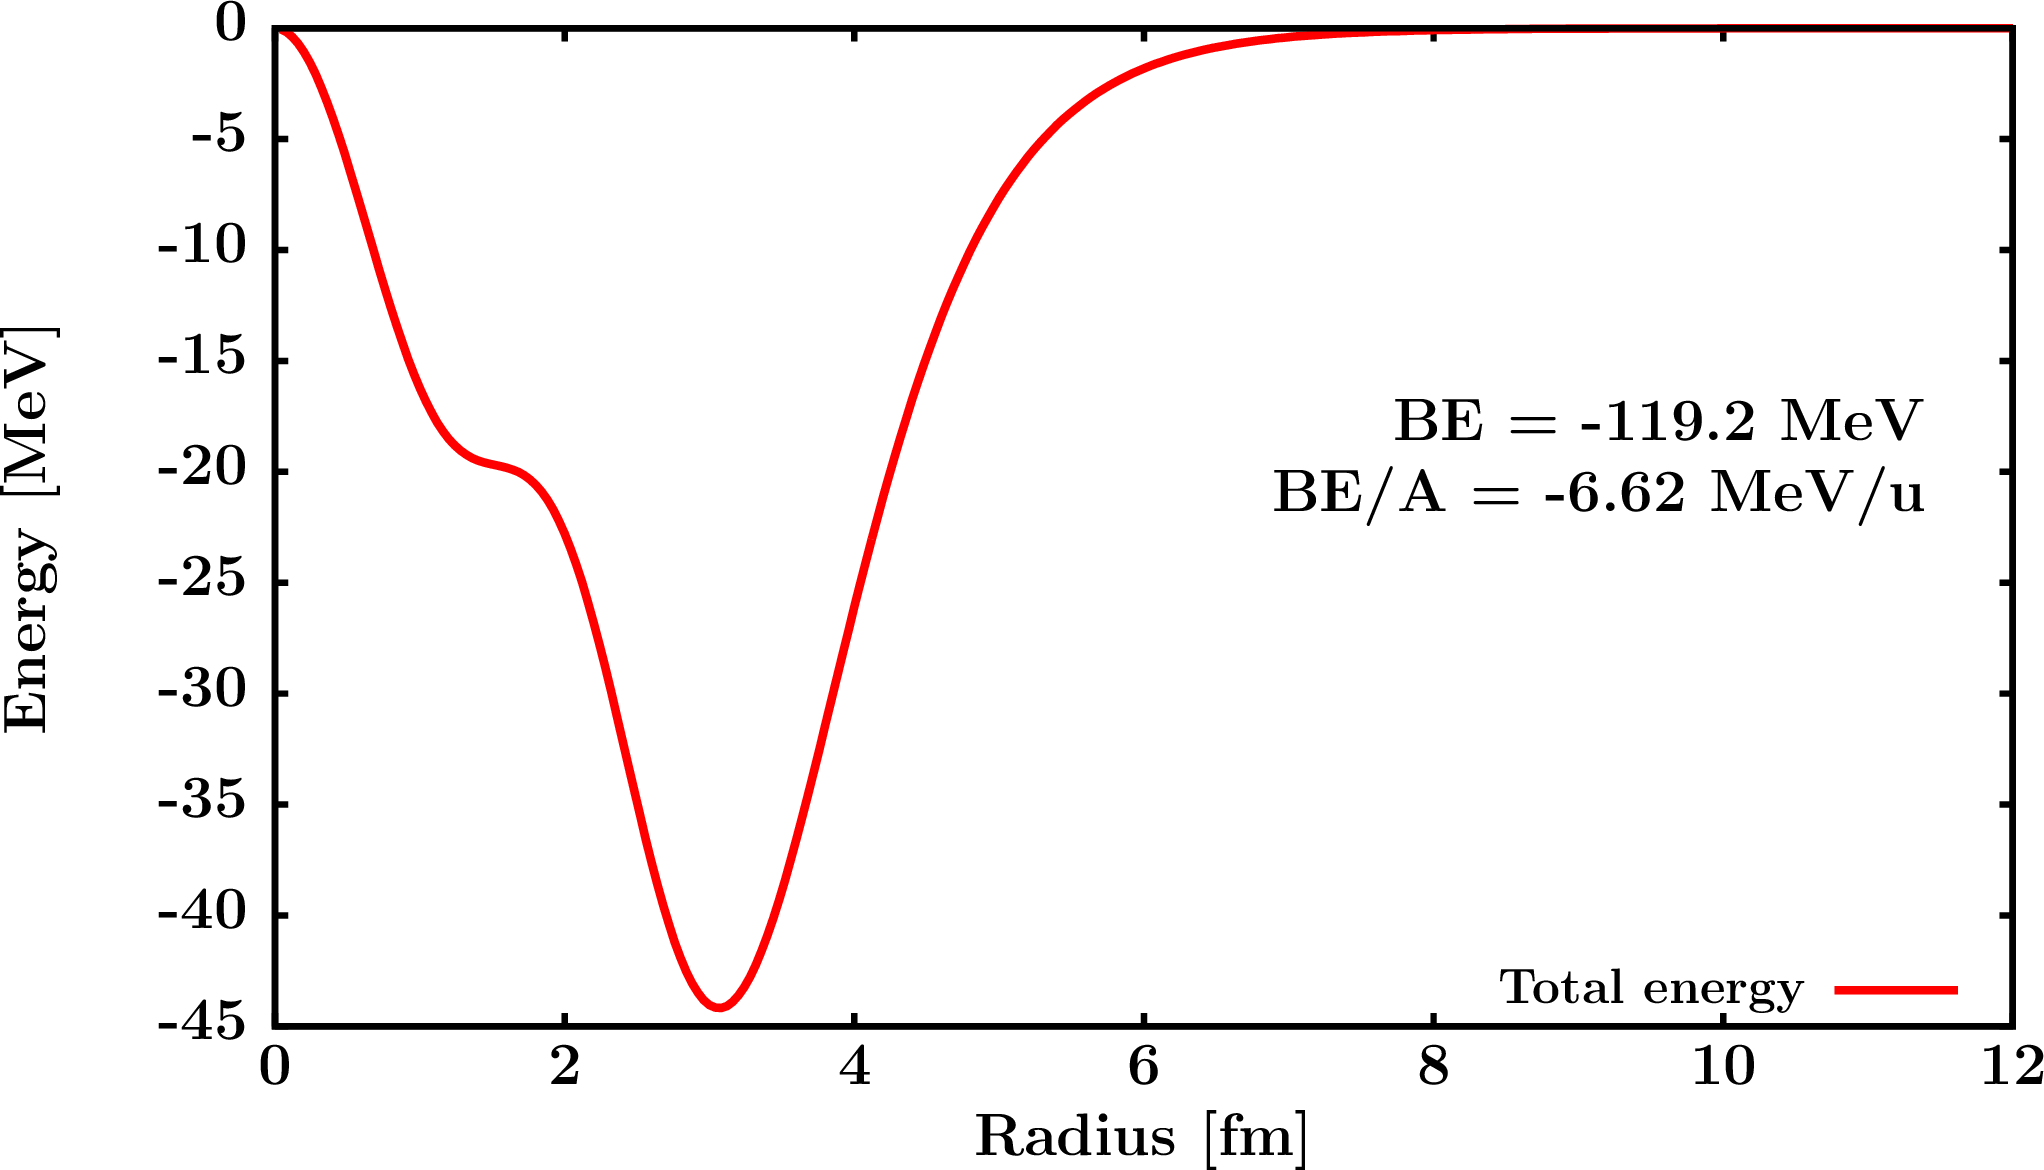
\includegraphics[width=\linewidth]{figures/o18_EnergyDistIntegral.png}
        \caption{\oEight\ energy distribution integral}
        \label{DOMFitData_o18_neutron_energyDistInt}
    \end{subfigure}\vspace{0.4in}
    \begin{subfigure}{0.70\textwidth}
        \centering
        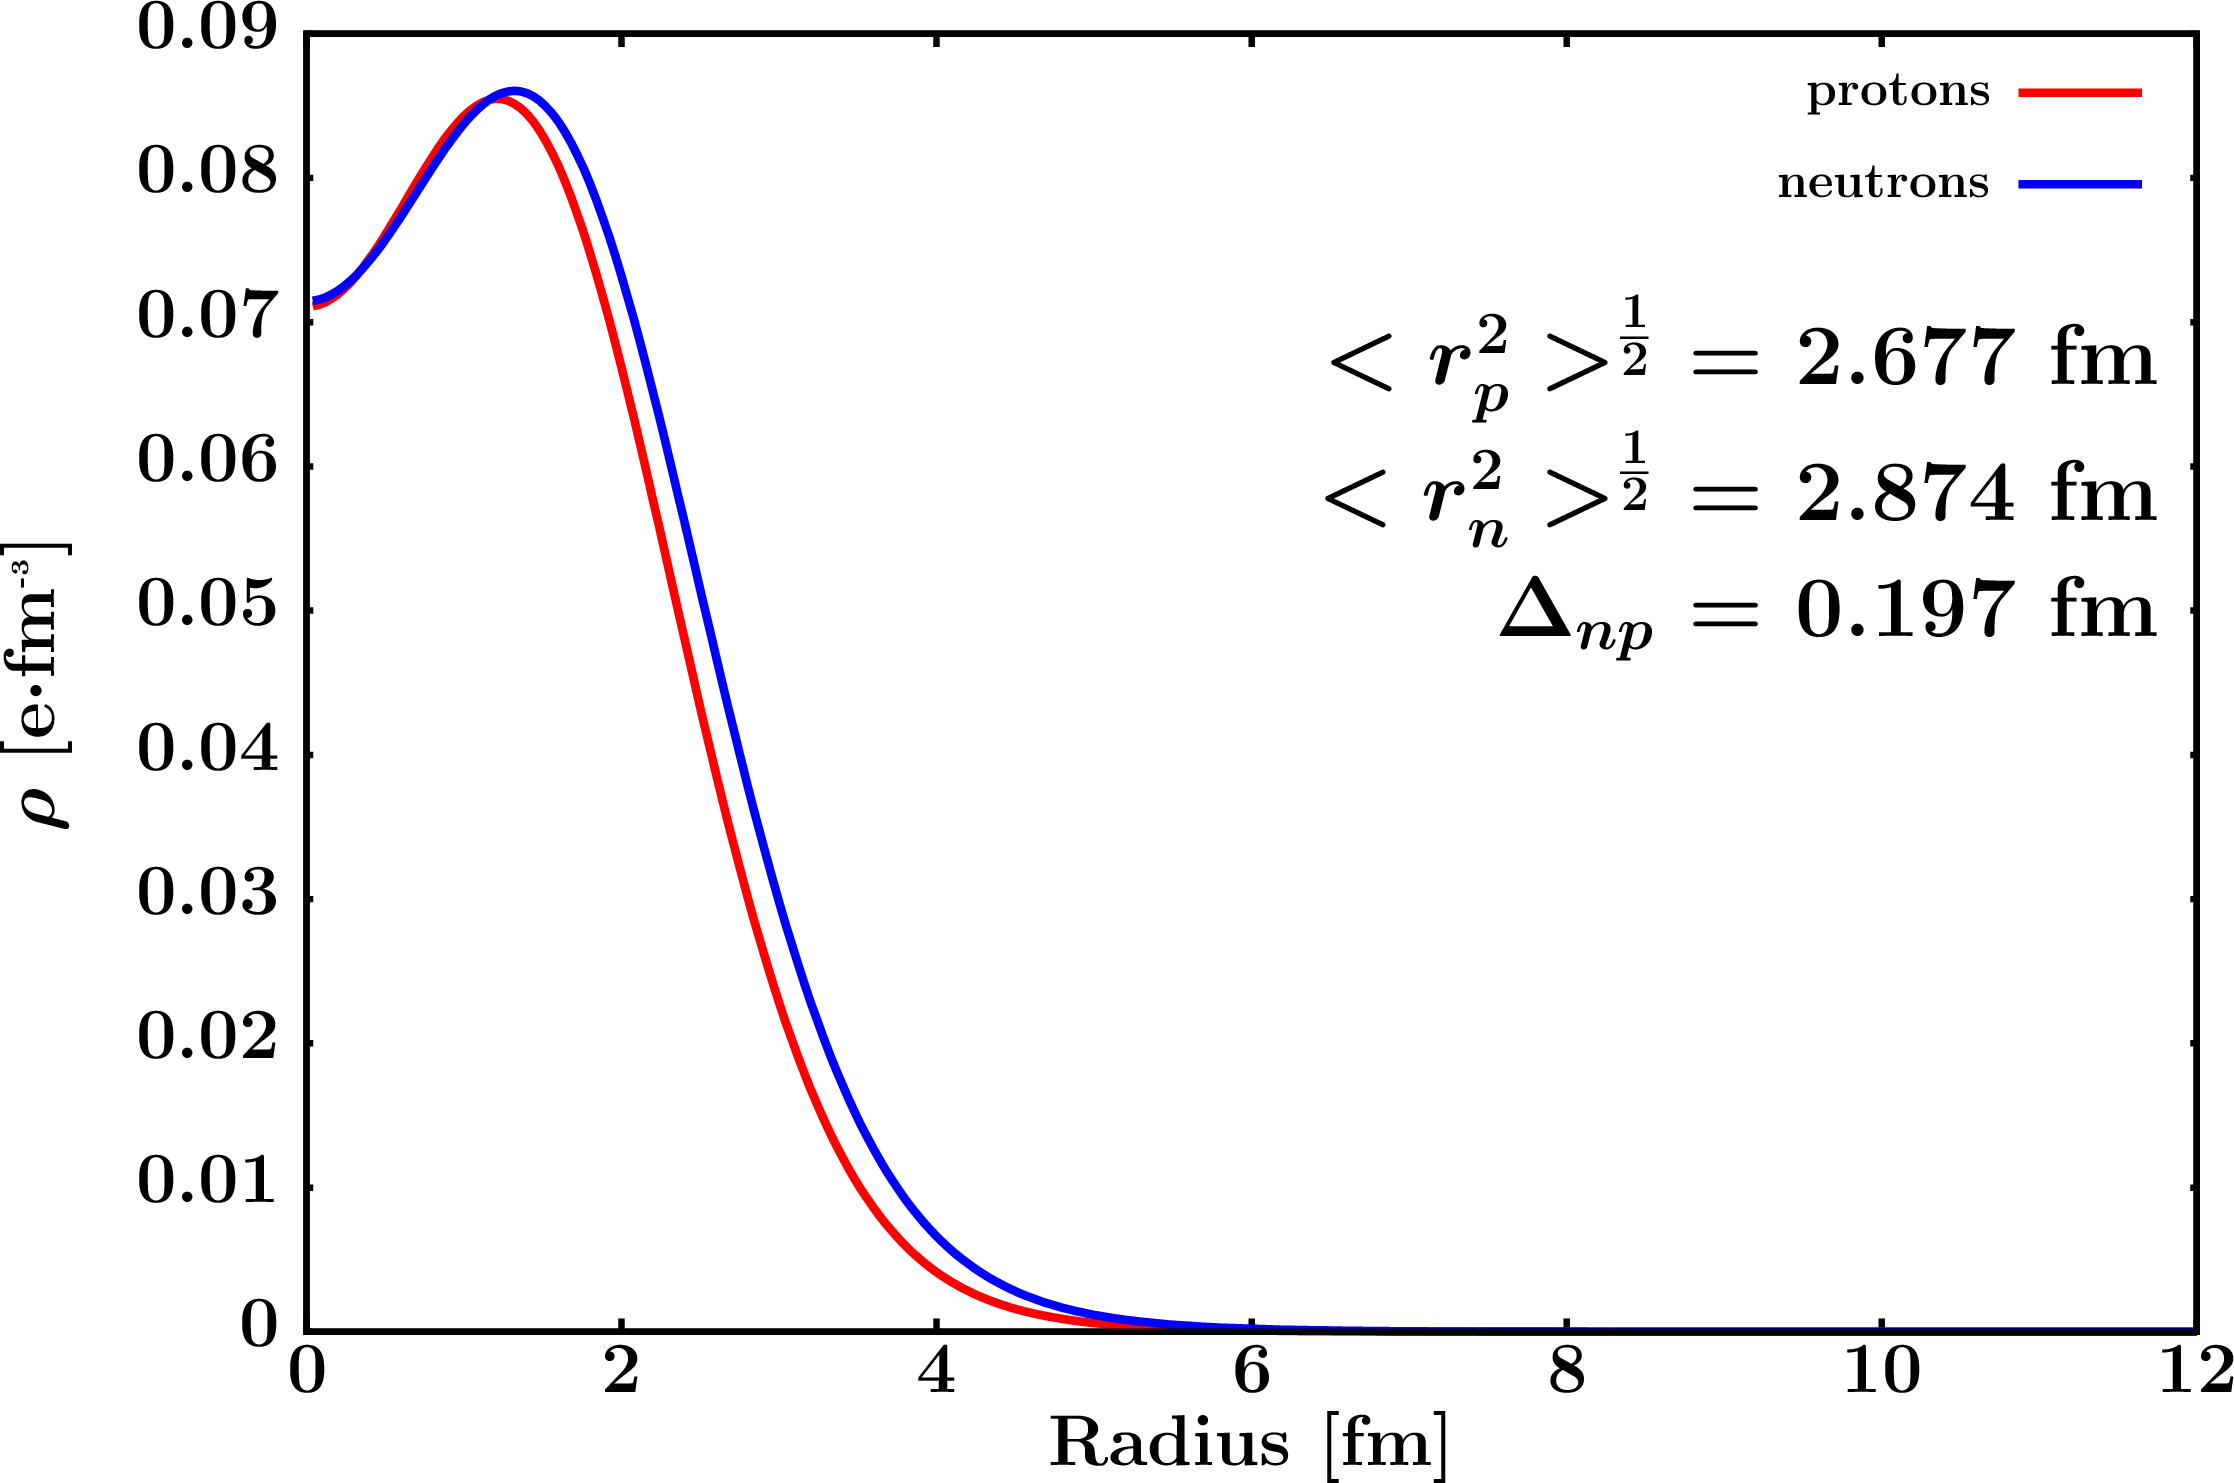
\includegraphics[width=\linewidth]{figures/o18_matterDensity.png}
        \caption{\oEight\ matter density distribution}
        \label{DOMFitData_o18_matterDensity}
    \end{subfigure}
\end{figure}

%\newpage
%\section{DOM fit of \caForty}
%\label{ca40DOMOutput}
%\begin{figure}[hbtp]
%    \captionsetup[subfigure]{labelformat=empty}
%    \centering
%    \begin{subfigure}[c]{0.39\textheight}
%        \centering
%        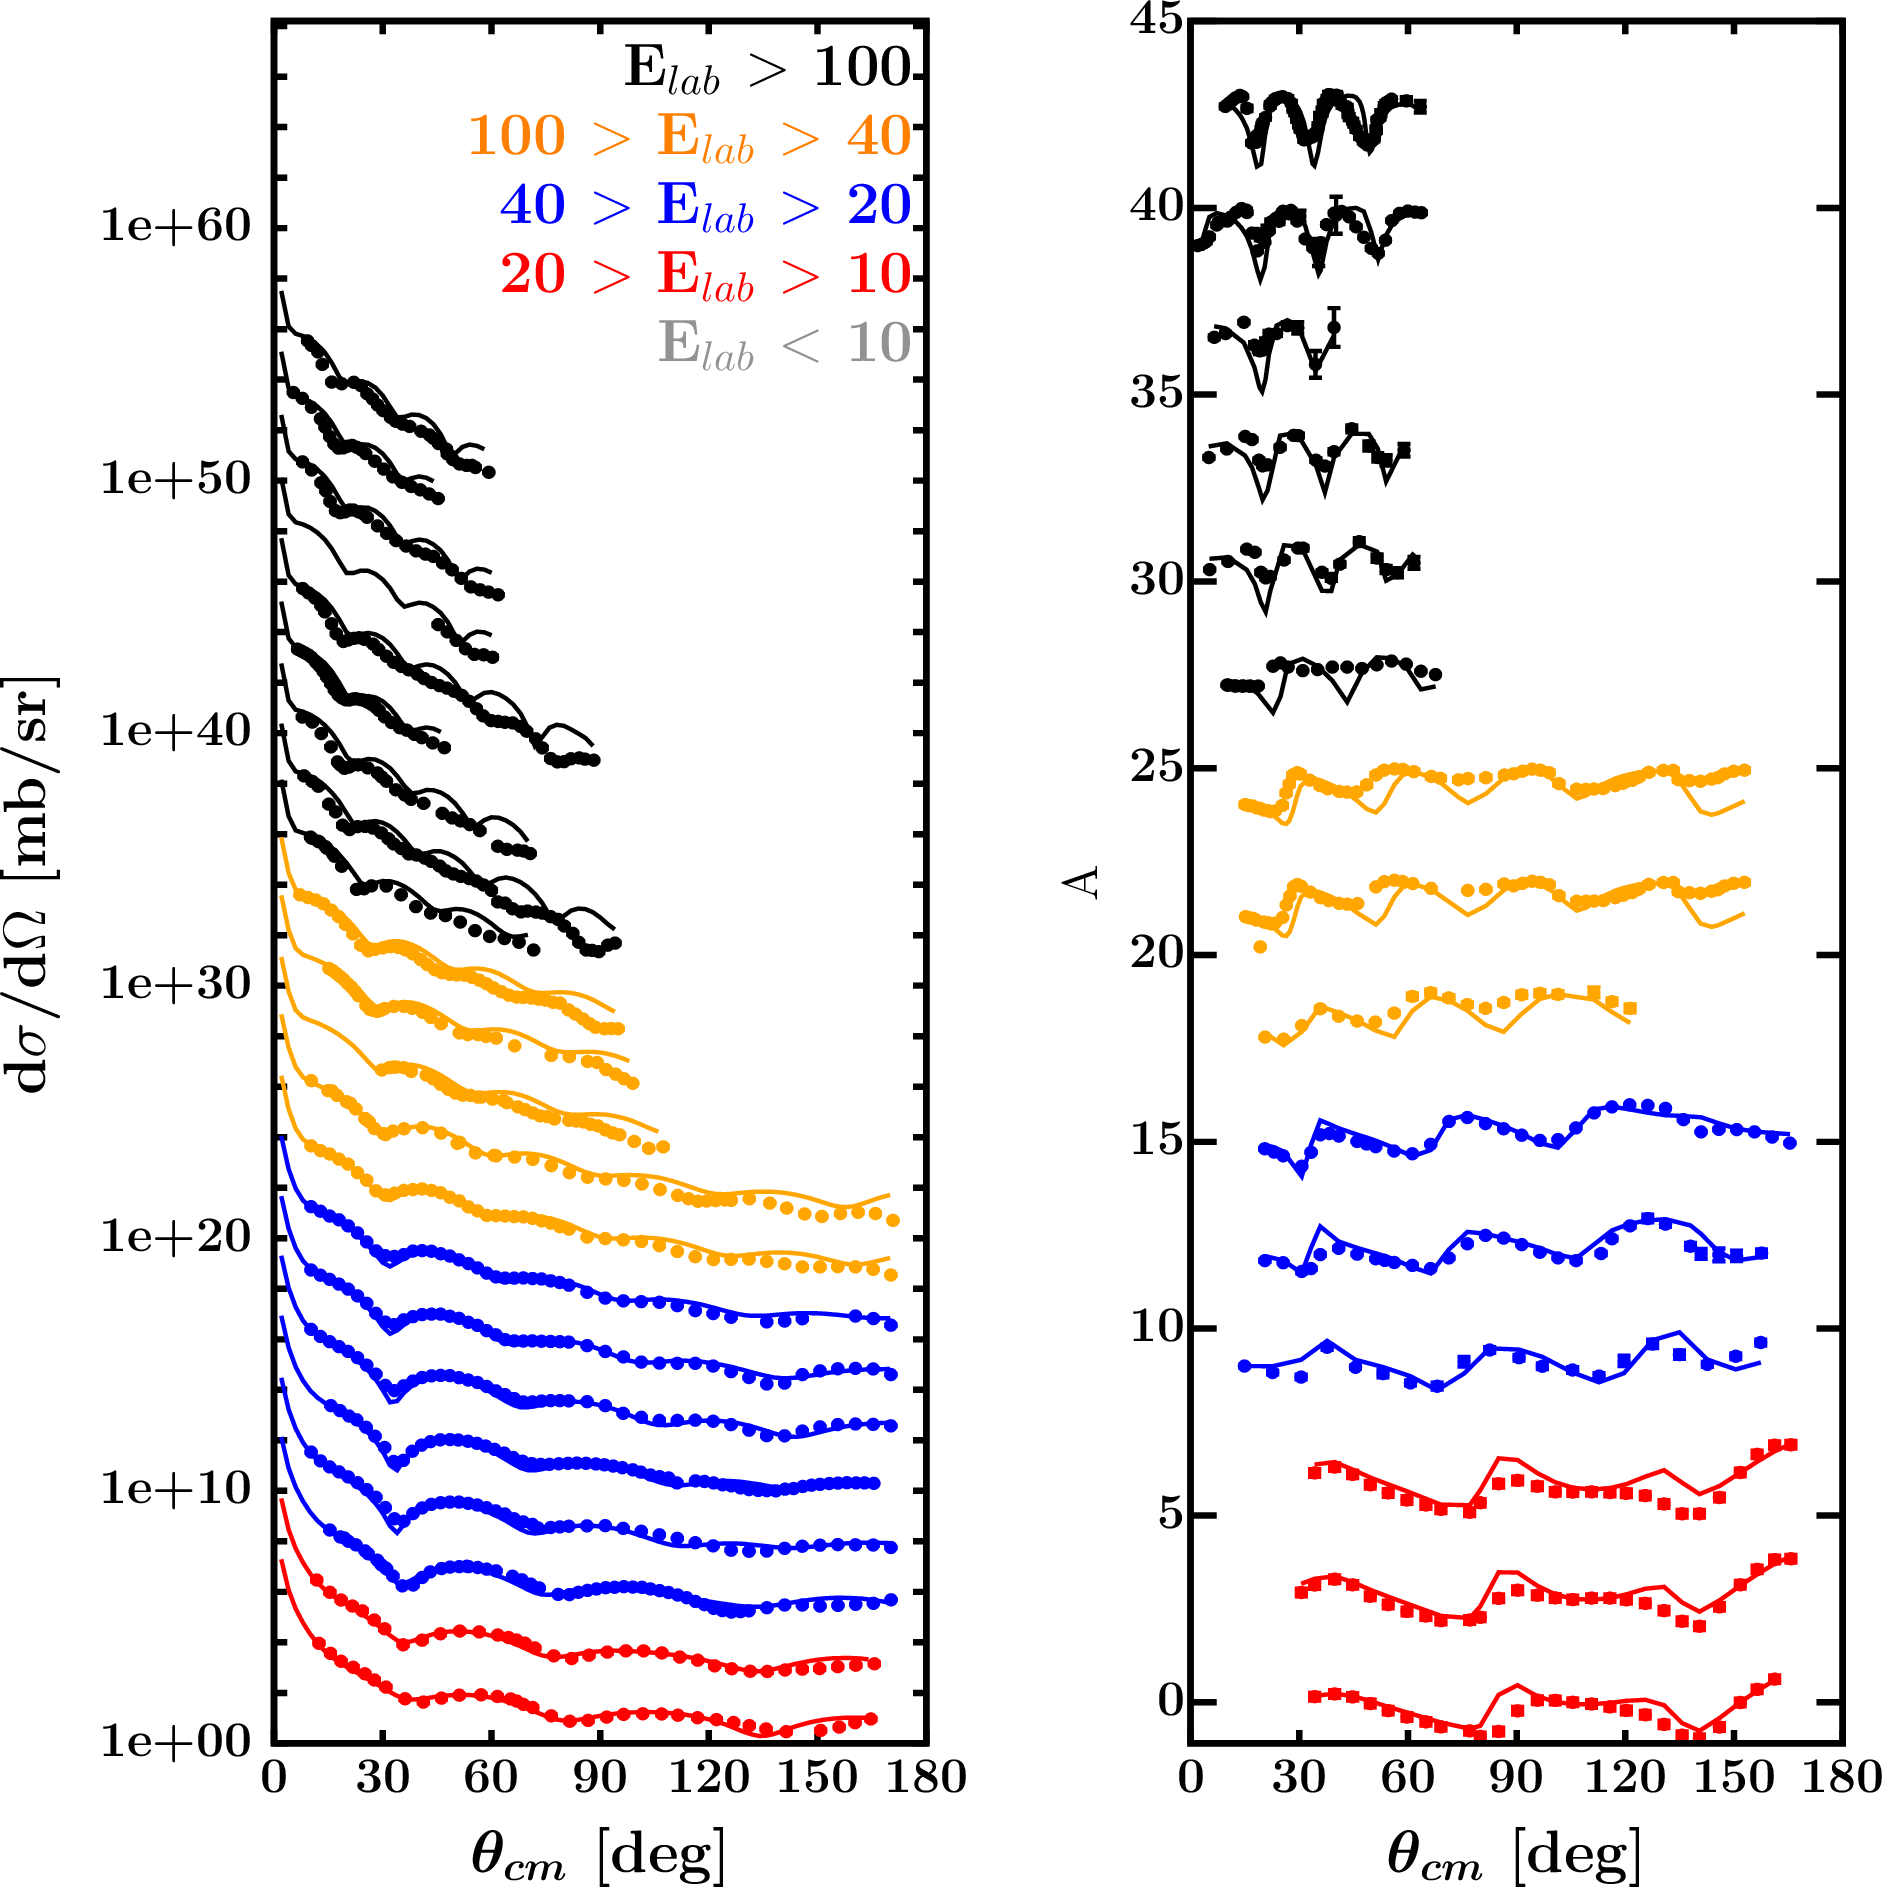
\includegraphics[width=\linewidth]{figures/ca40_protonElastic.png}
%        \caption{\caForty\ proton elastic scattering}
%        \label{DOMFitData_ca40_proton_elastic}
%    \end{subfigure}\hspace{6pt}
%    \begin{subfigure}[c]{0.39\textheight}
%        \centering
%        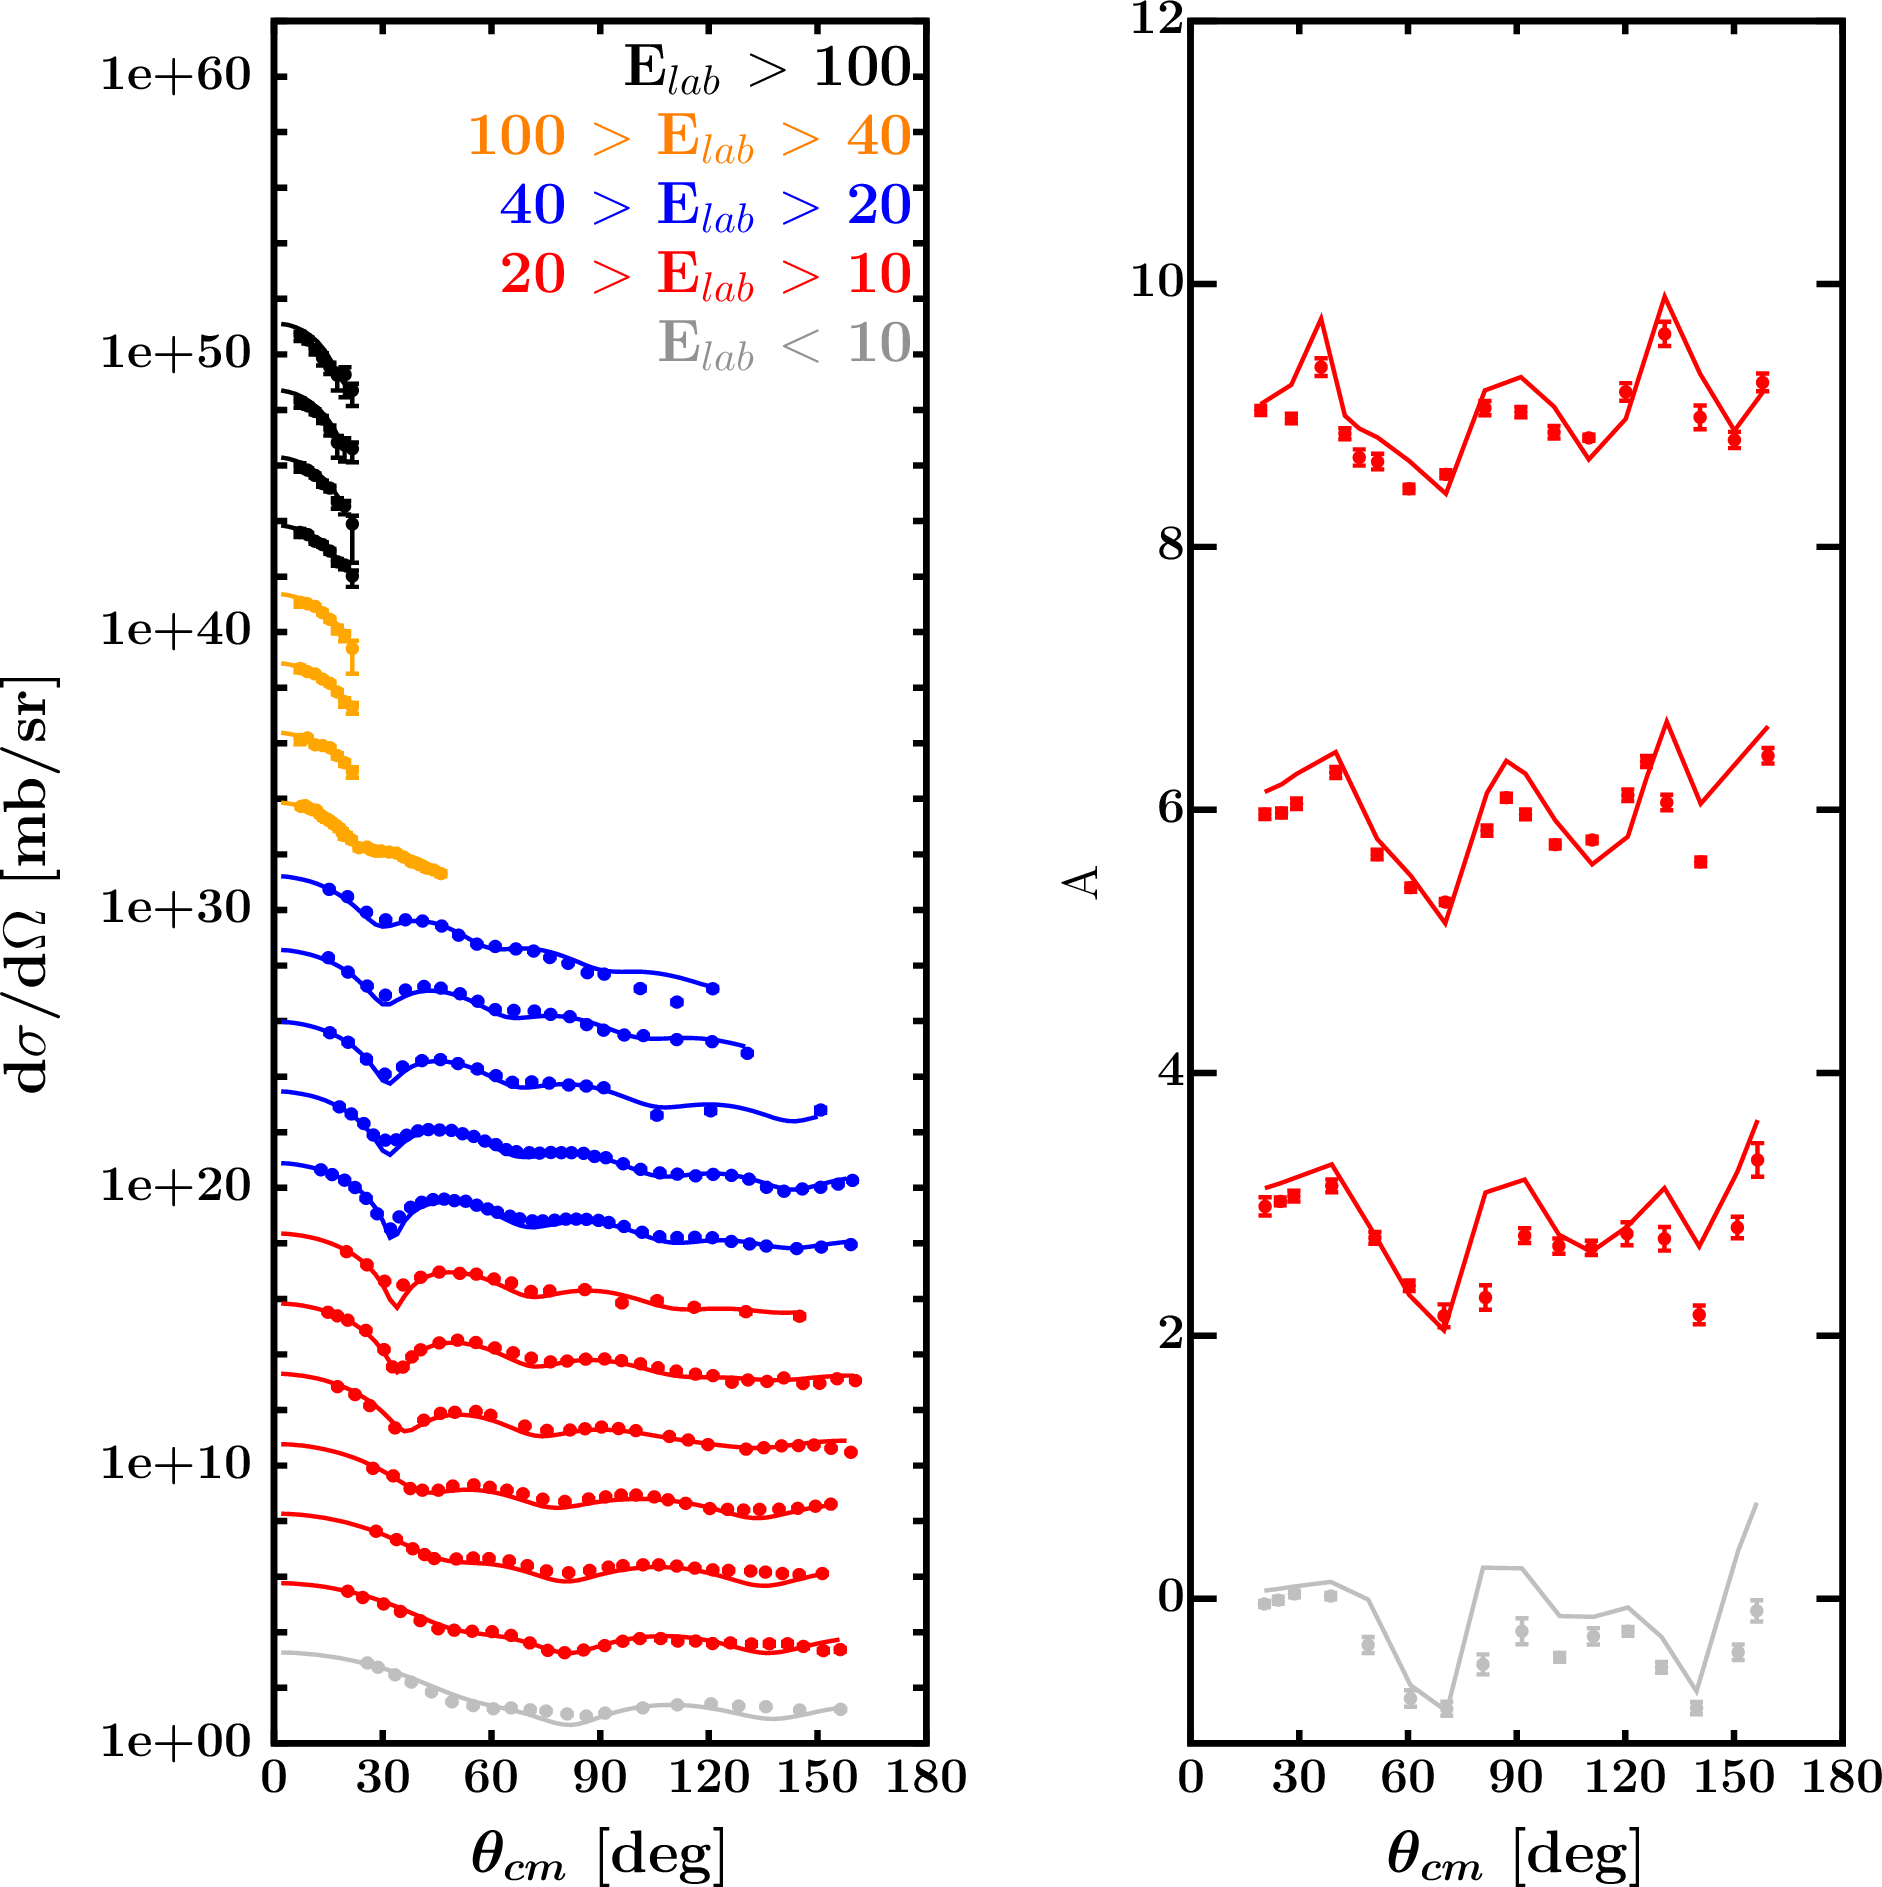
\includegraphics[width=0.52\linewidth]{figures/ca40_neutronElastic.png}
%        \caption{\caForty\ neutron elastic scattering}
%        \label{DOMFitData_ca40_neutron_elastic}
%    \end{subfigure}\vspace{0.70in}
%    \begin{subfigure}[c]{0.45\textwidth}
%        \centering
%        %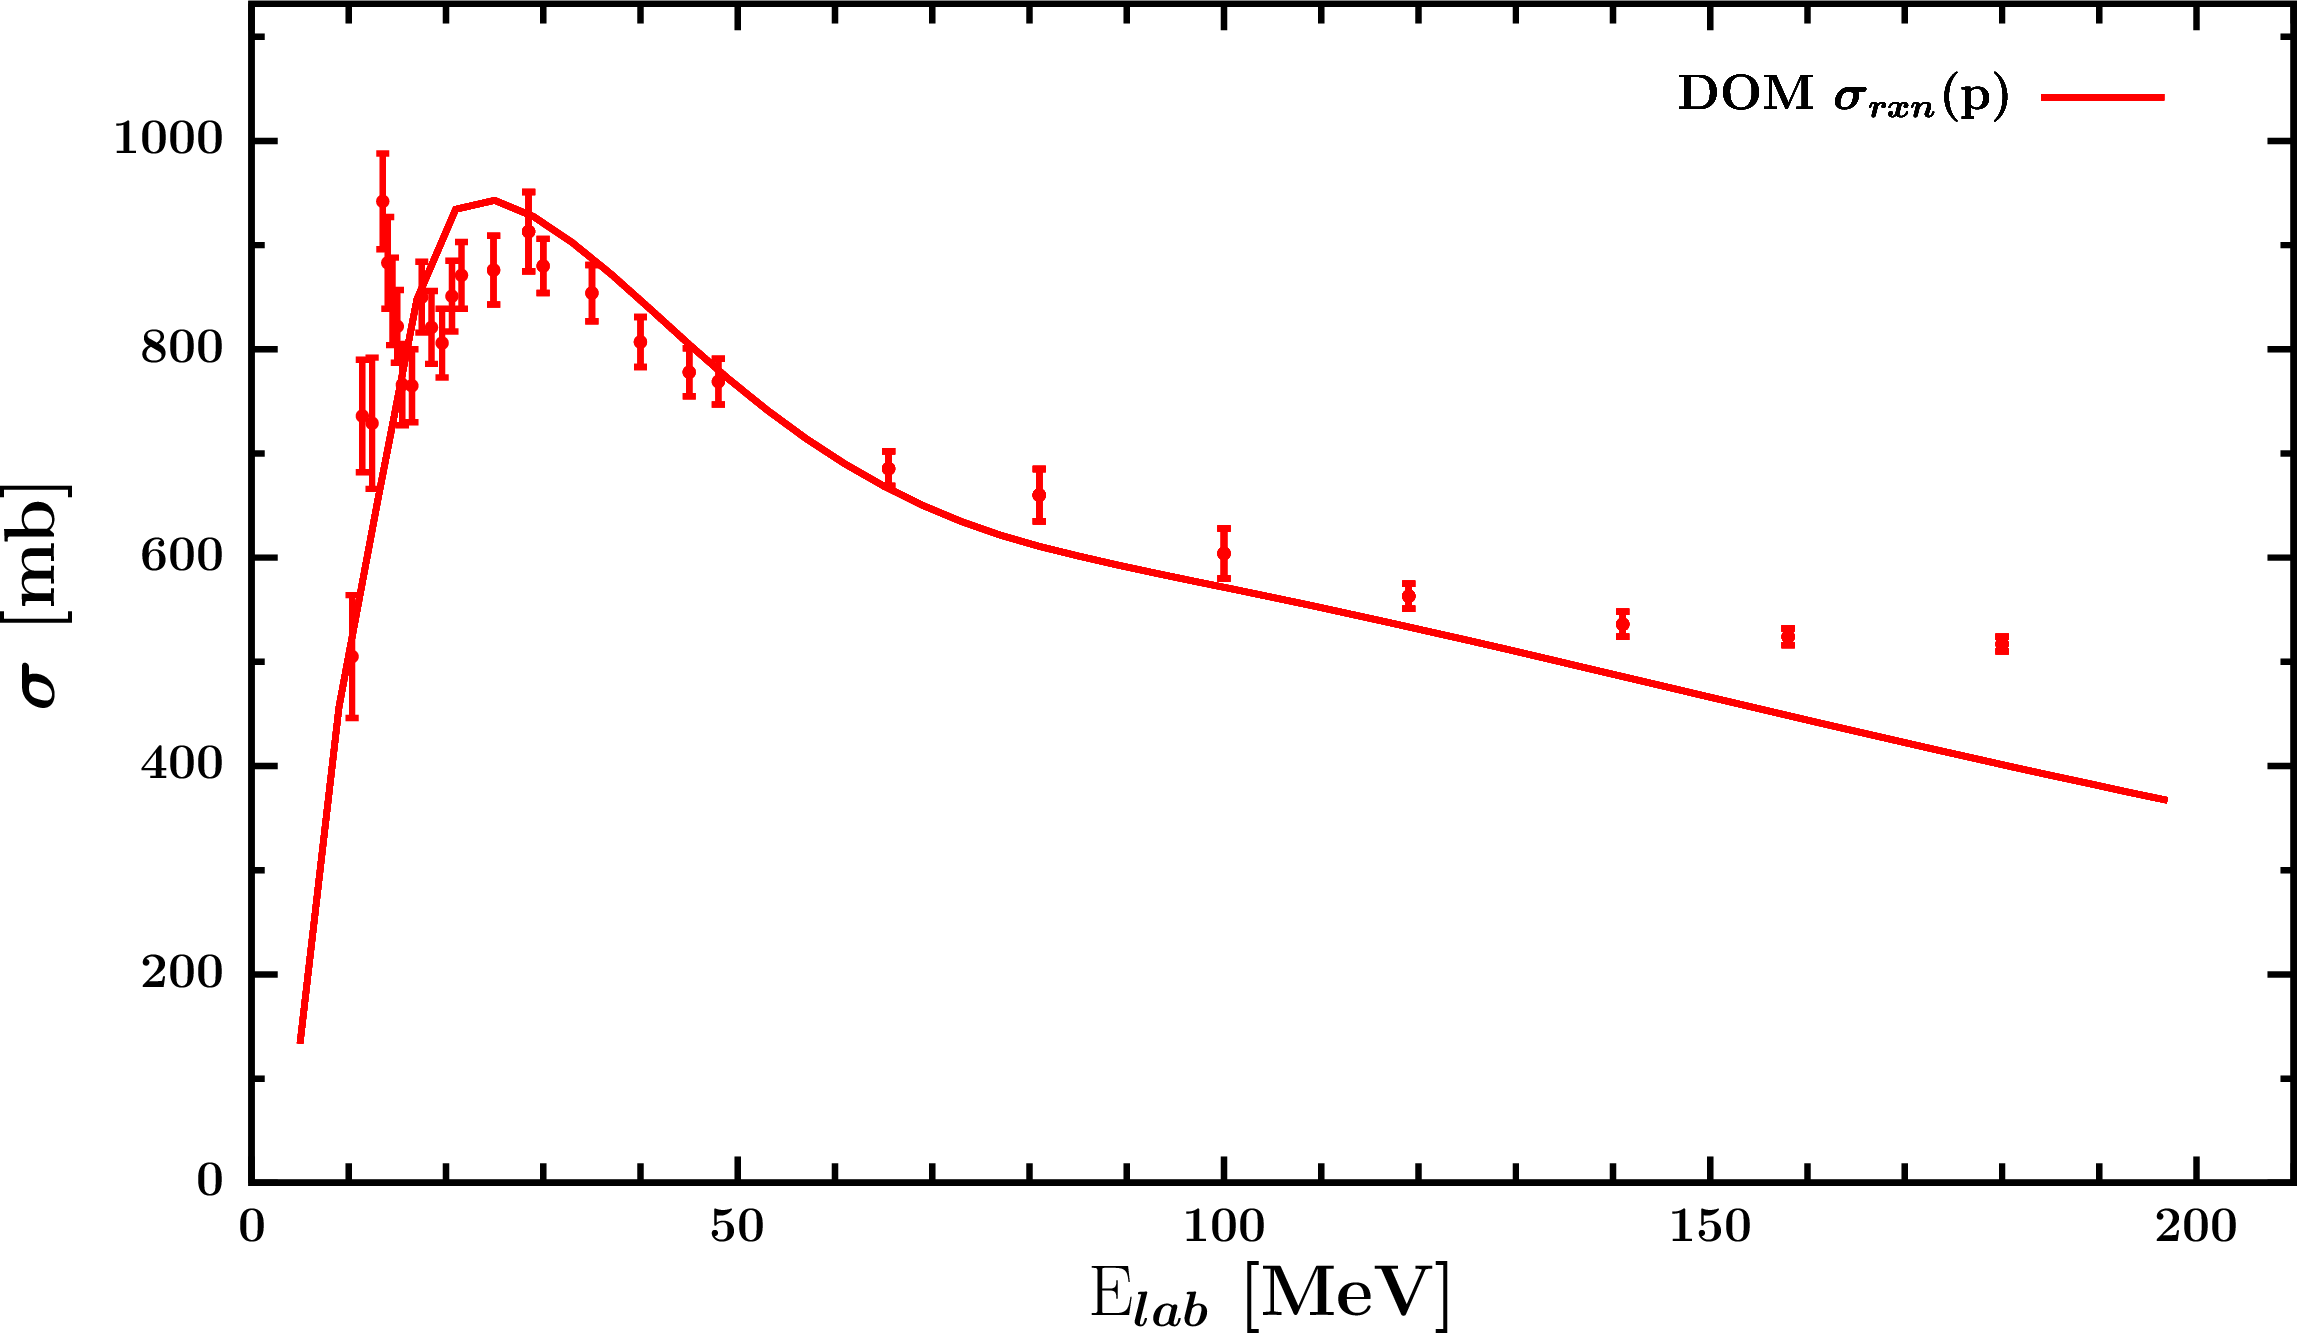
\includegraphics[width=\linewidth]{figures/ca40_protonInelastic.png}
%        \caption{No \caForty\ proton \rxn\\ data were available}
%        \label{DOMFitData_ca40_proton_inelastic}
%    \end{subfigure}\hspace{6pt}
%    \begin{subfigure}[c]{0.45\textwidth}
%        \centering
%        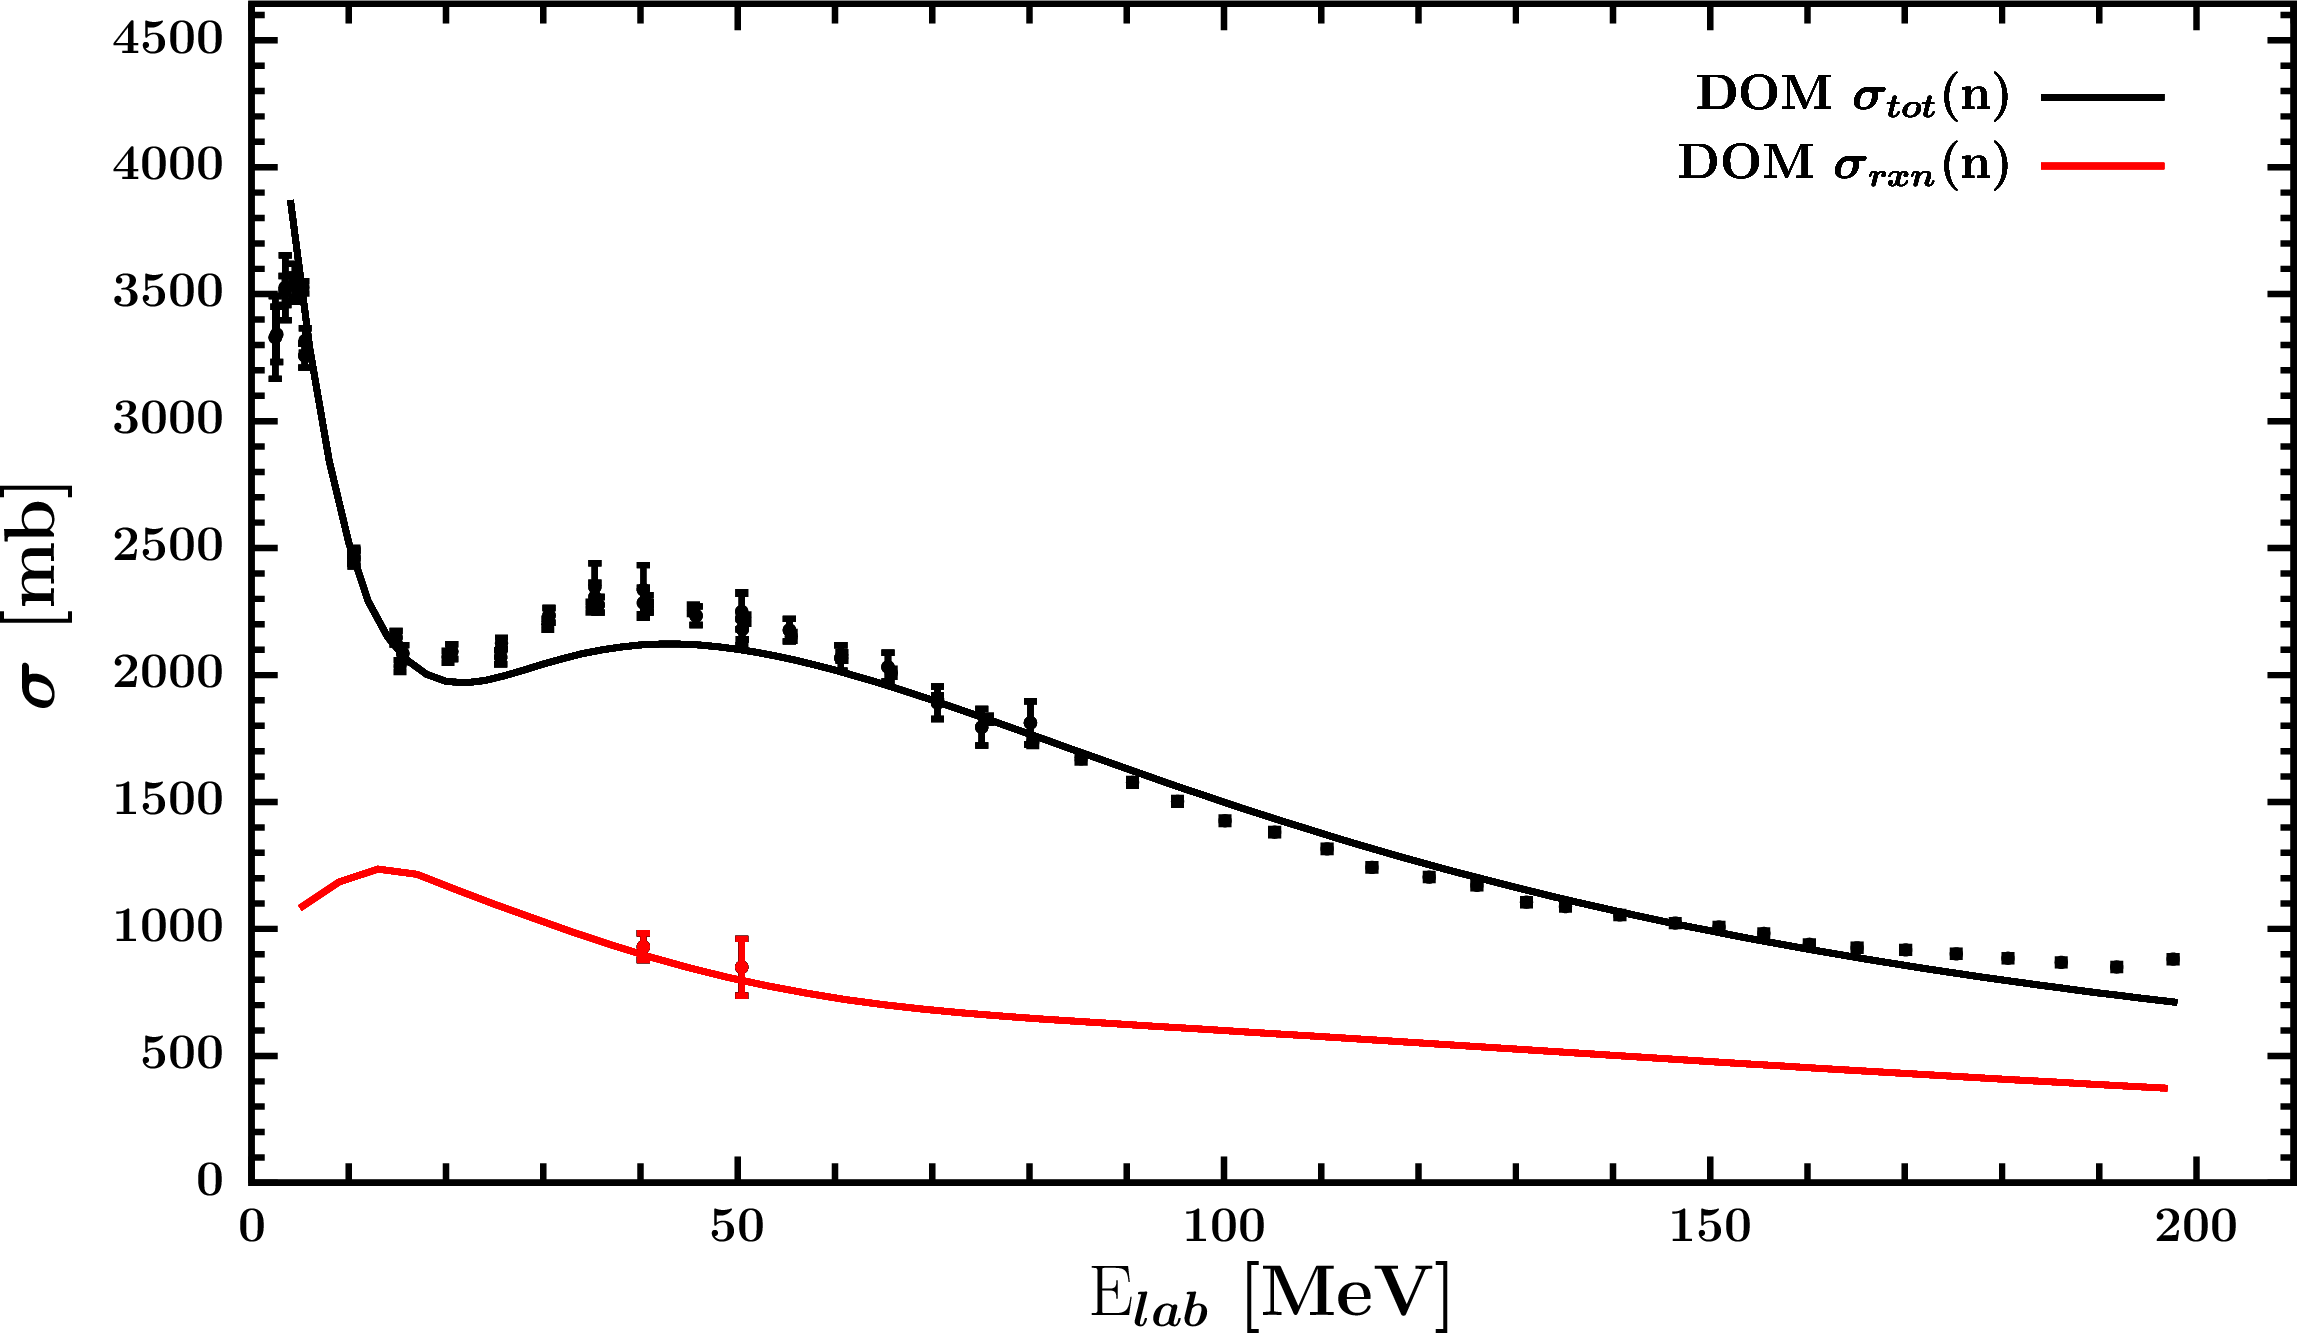
\includegraphics[width=\linewidth]{figures/ca40_neutronInelastic.png}
%        \caption{\caForty\ neutron \rxn\ and \tot}
%        \label{DOMFitData_ca40_neutron_inelastic}
%    \end{subfigure}
%\end{figure}
%\afterpage{\clearpage}
%\begin{figure}[hbtp]
%    \captionsetup[subfigure]{labelformat=empty}
%    \centering
%    \begin{subfigure}[b]{0.45\textwidth}
%        \centering
%        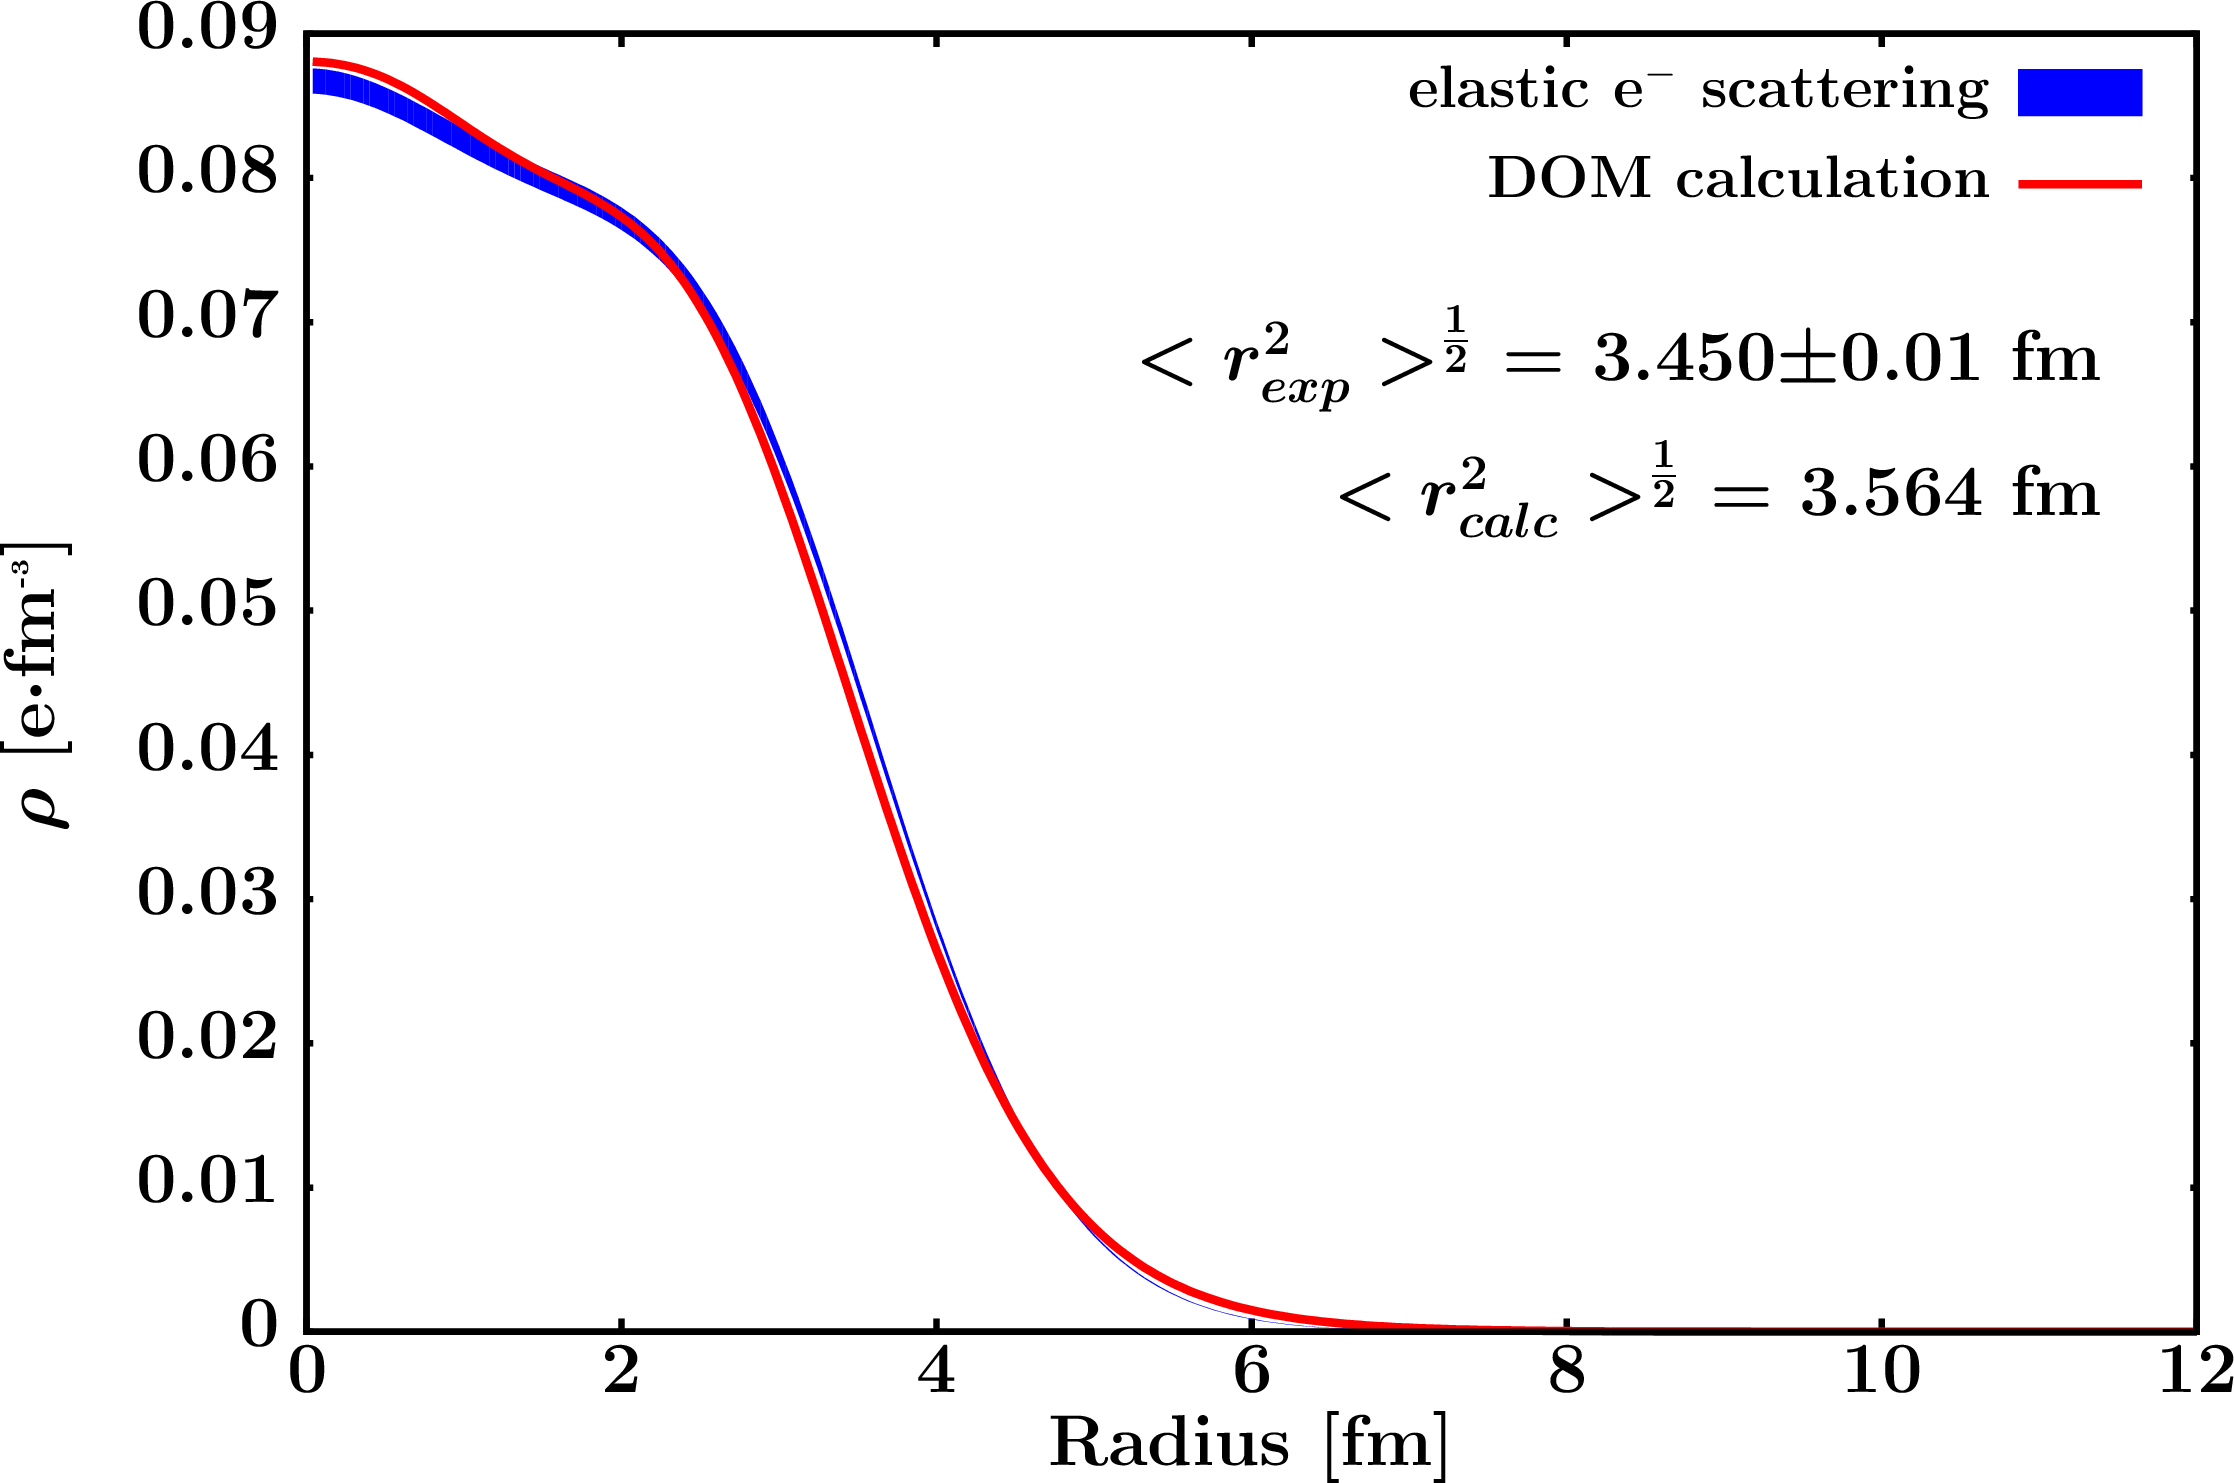
\includegraphics[width=\linewidth]{figures/ca40_chargeDensity.png}
%        \caption{\caForty\ charge density}
%        \label{DOMFitData_ca40_chargeDensity}
%    \end{subfigure}\hspace{6pt}
%    \begin{subfigure}[b]{0.45\textwidth}
%        \centering
%        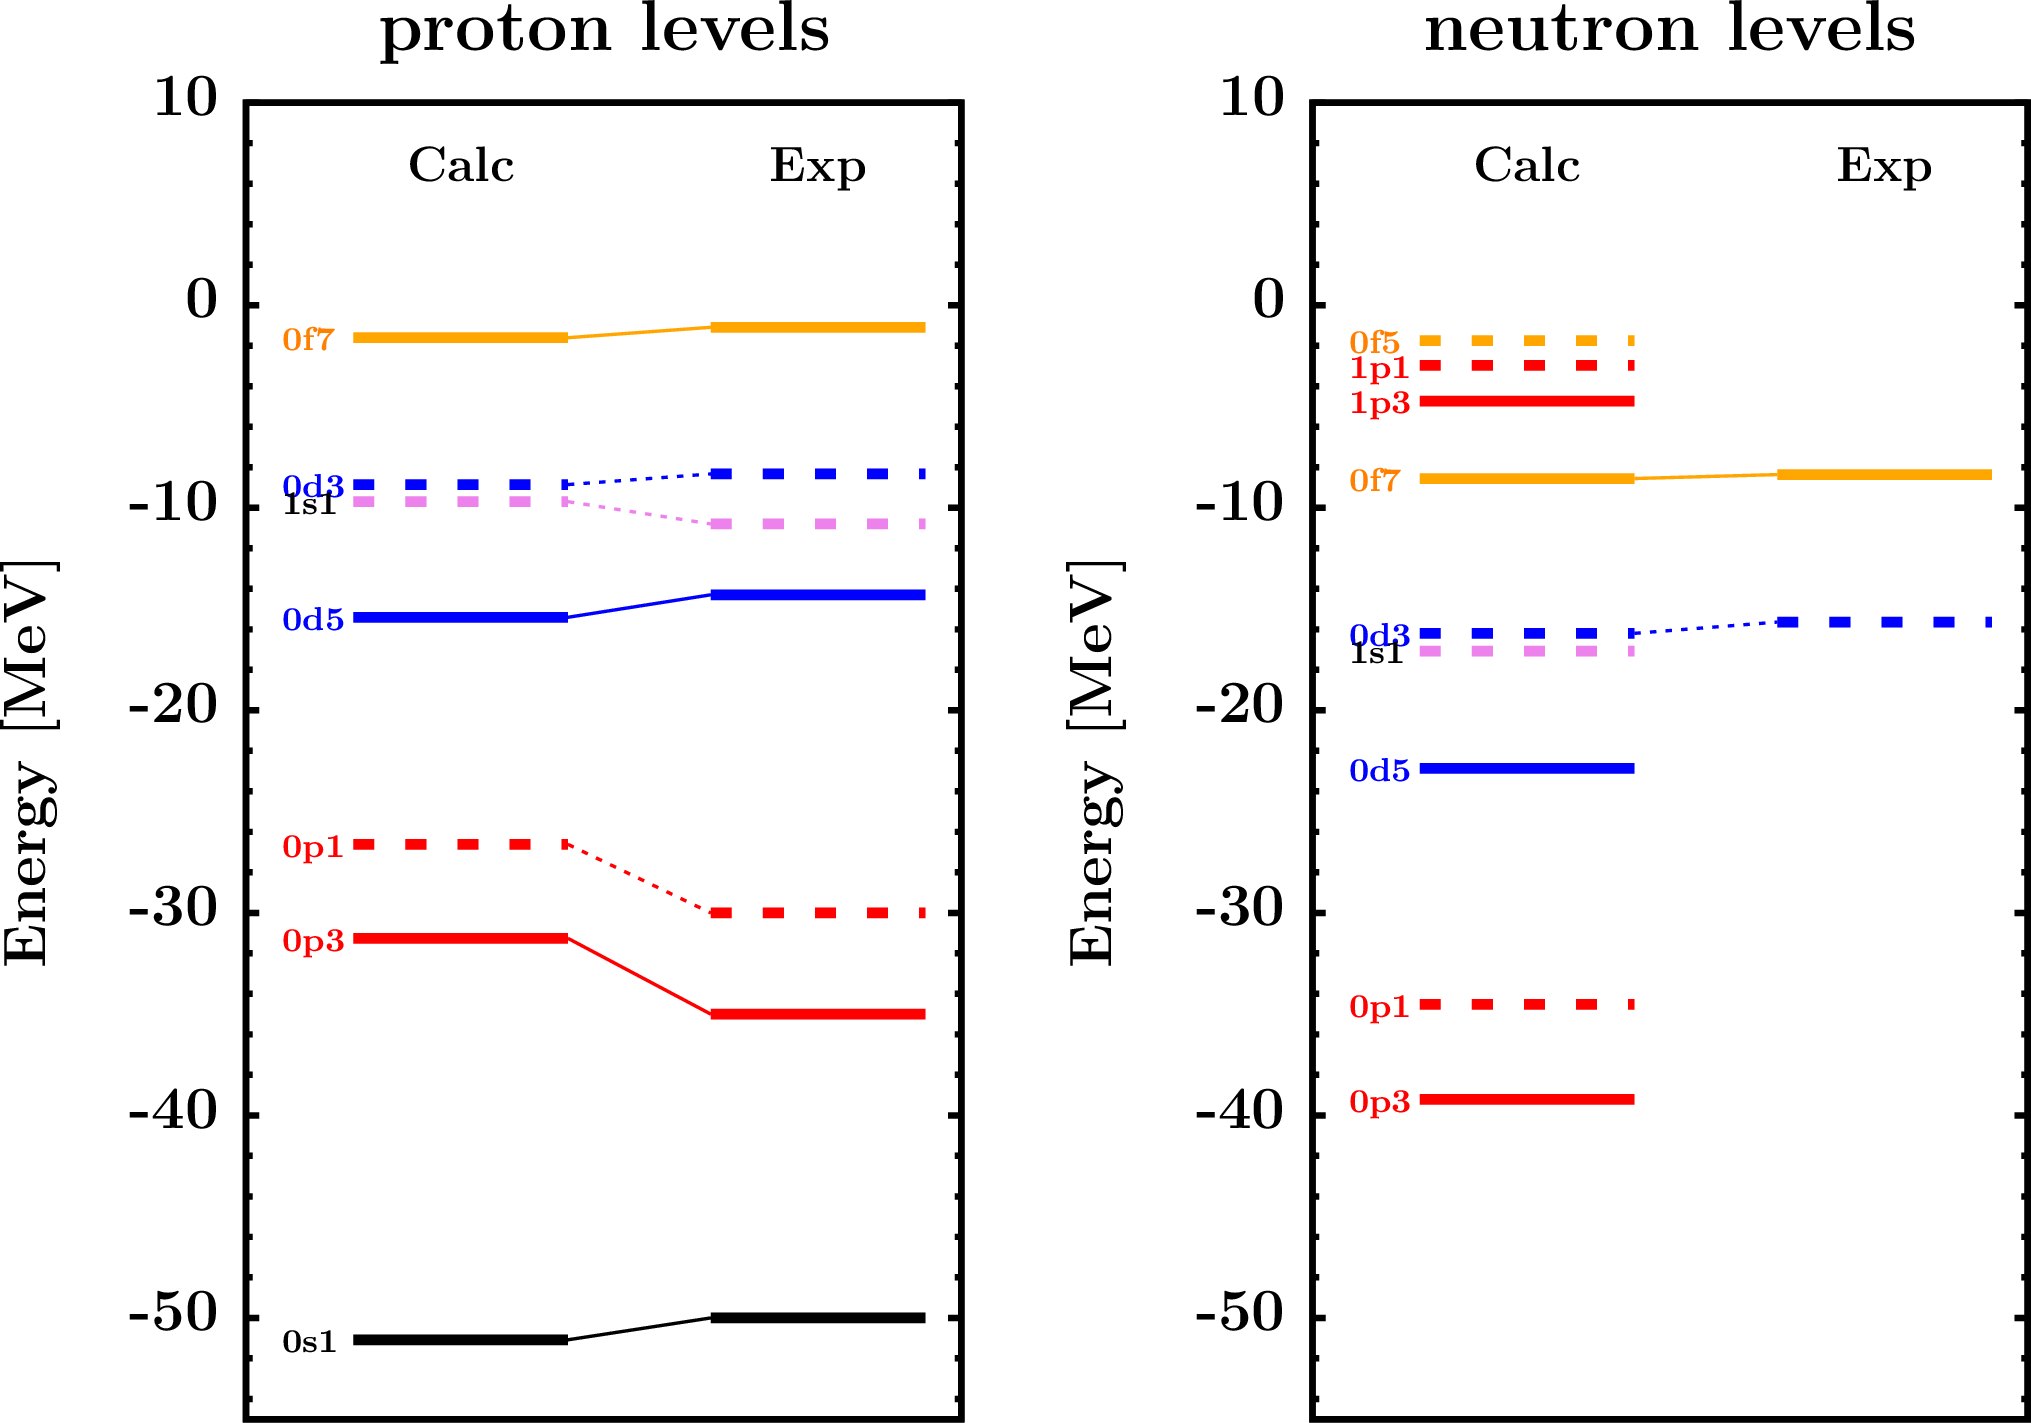
\includegraphics[width=\linewidth]{figures/ca40_SPLevels.png}
%        \caption{\caForty\ single-particle levels}
%        \label{DOMFitData_ca40_SPLevels}
%    \end{subfigure}\vspace{0.3in}
%    \begin{subfigure}[b]{0.45\textwidth}
%        \centering
%        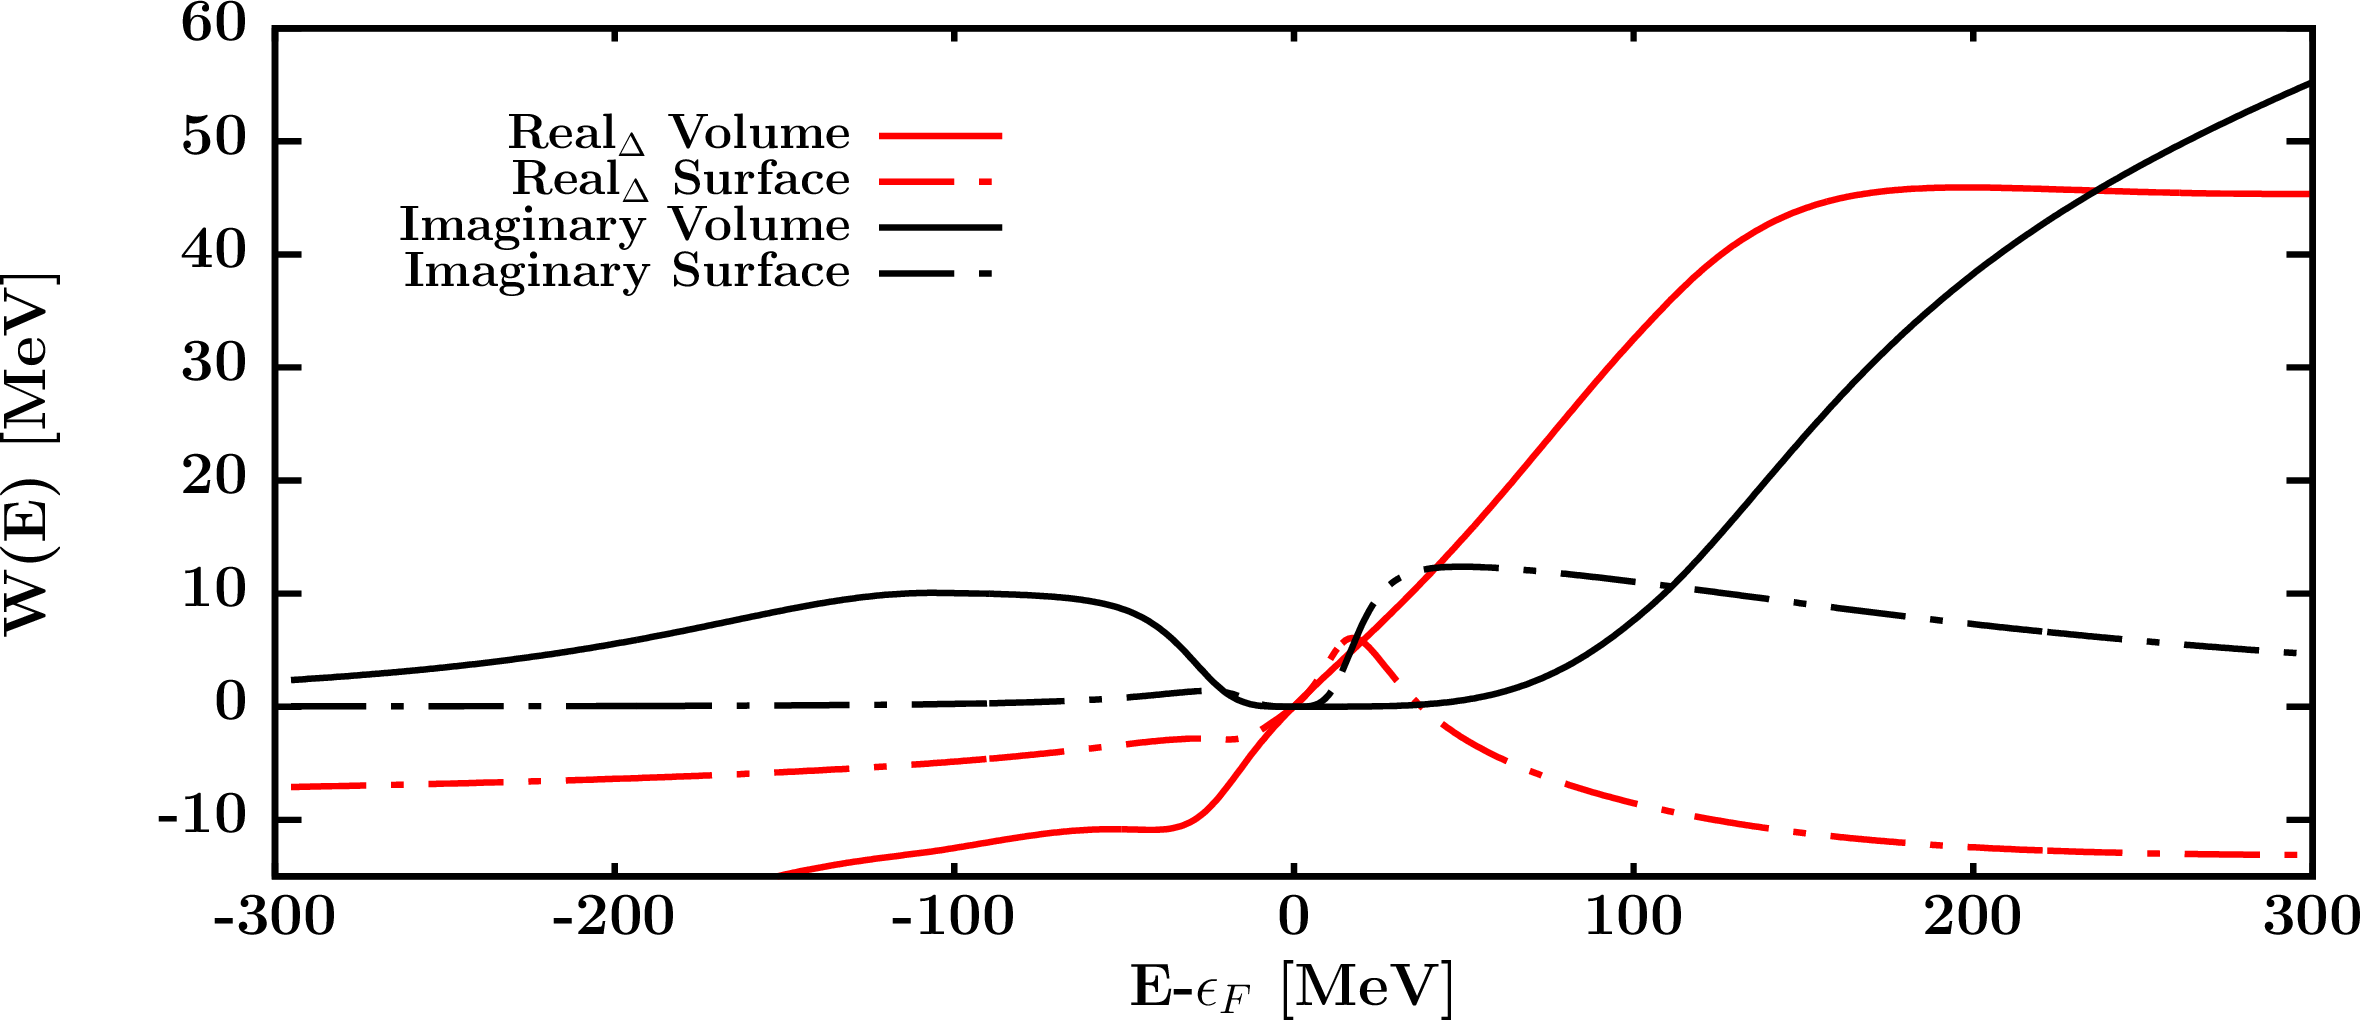
\includegraphics[width=\linewidth]{figures/ca40_protonPotentials.png}
%        \caption{\caForty\ proton potential energy-dependence}
%        \label{DOMFitData_ca40_proton_potentialComponent_energy}
%    \end{subfigure}\hspace{6pt}
%    \begin{subfigure}[b]{0.45\linewidth}
%        \centering
%        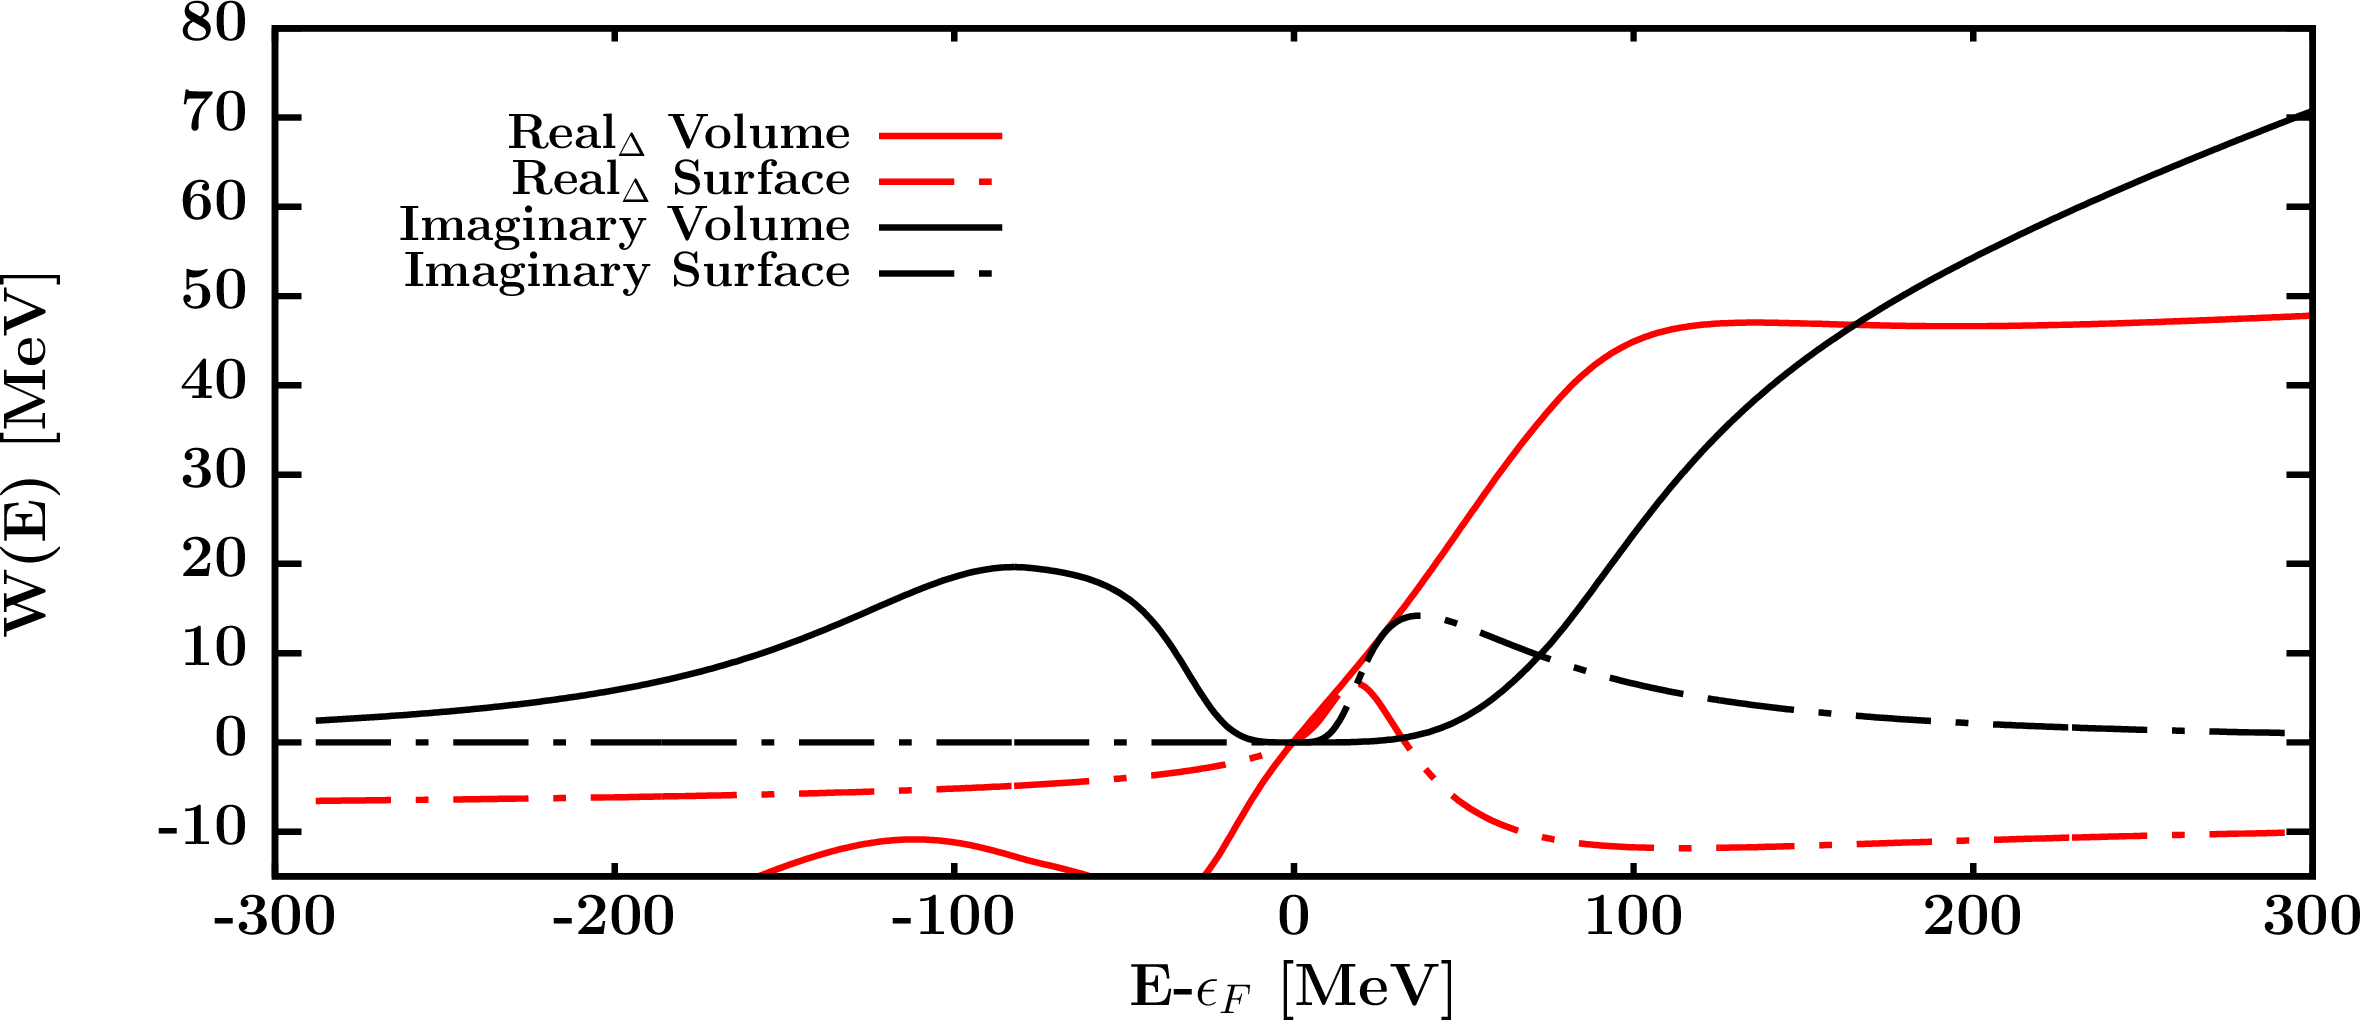
\includegraphics[width=\linewidth]{figures/ca40_neutronPotentials.png}
%        \caption{\caForty\ neutron potential energy-dependence}
%        \label{DOMFitData_ca40_neutron_potentialComponent_energy}
%    \end{subfigure}\vspace{0.3in}
%    \begin{subfigure}[b]{0.45\textwidth}
%        \centering
%        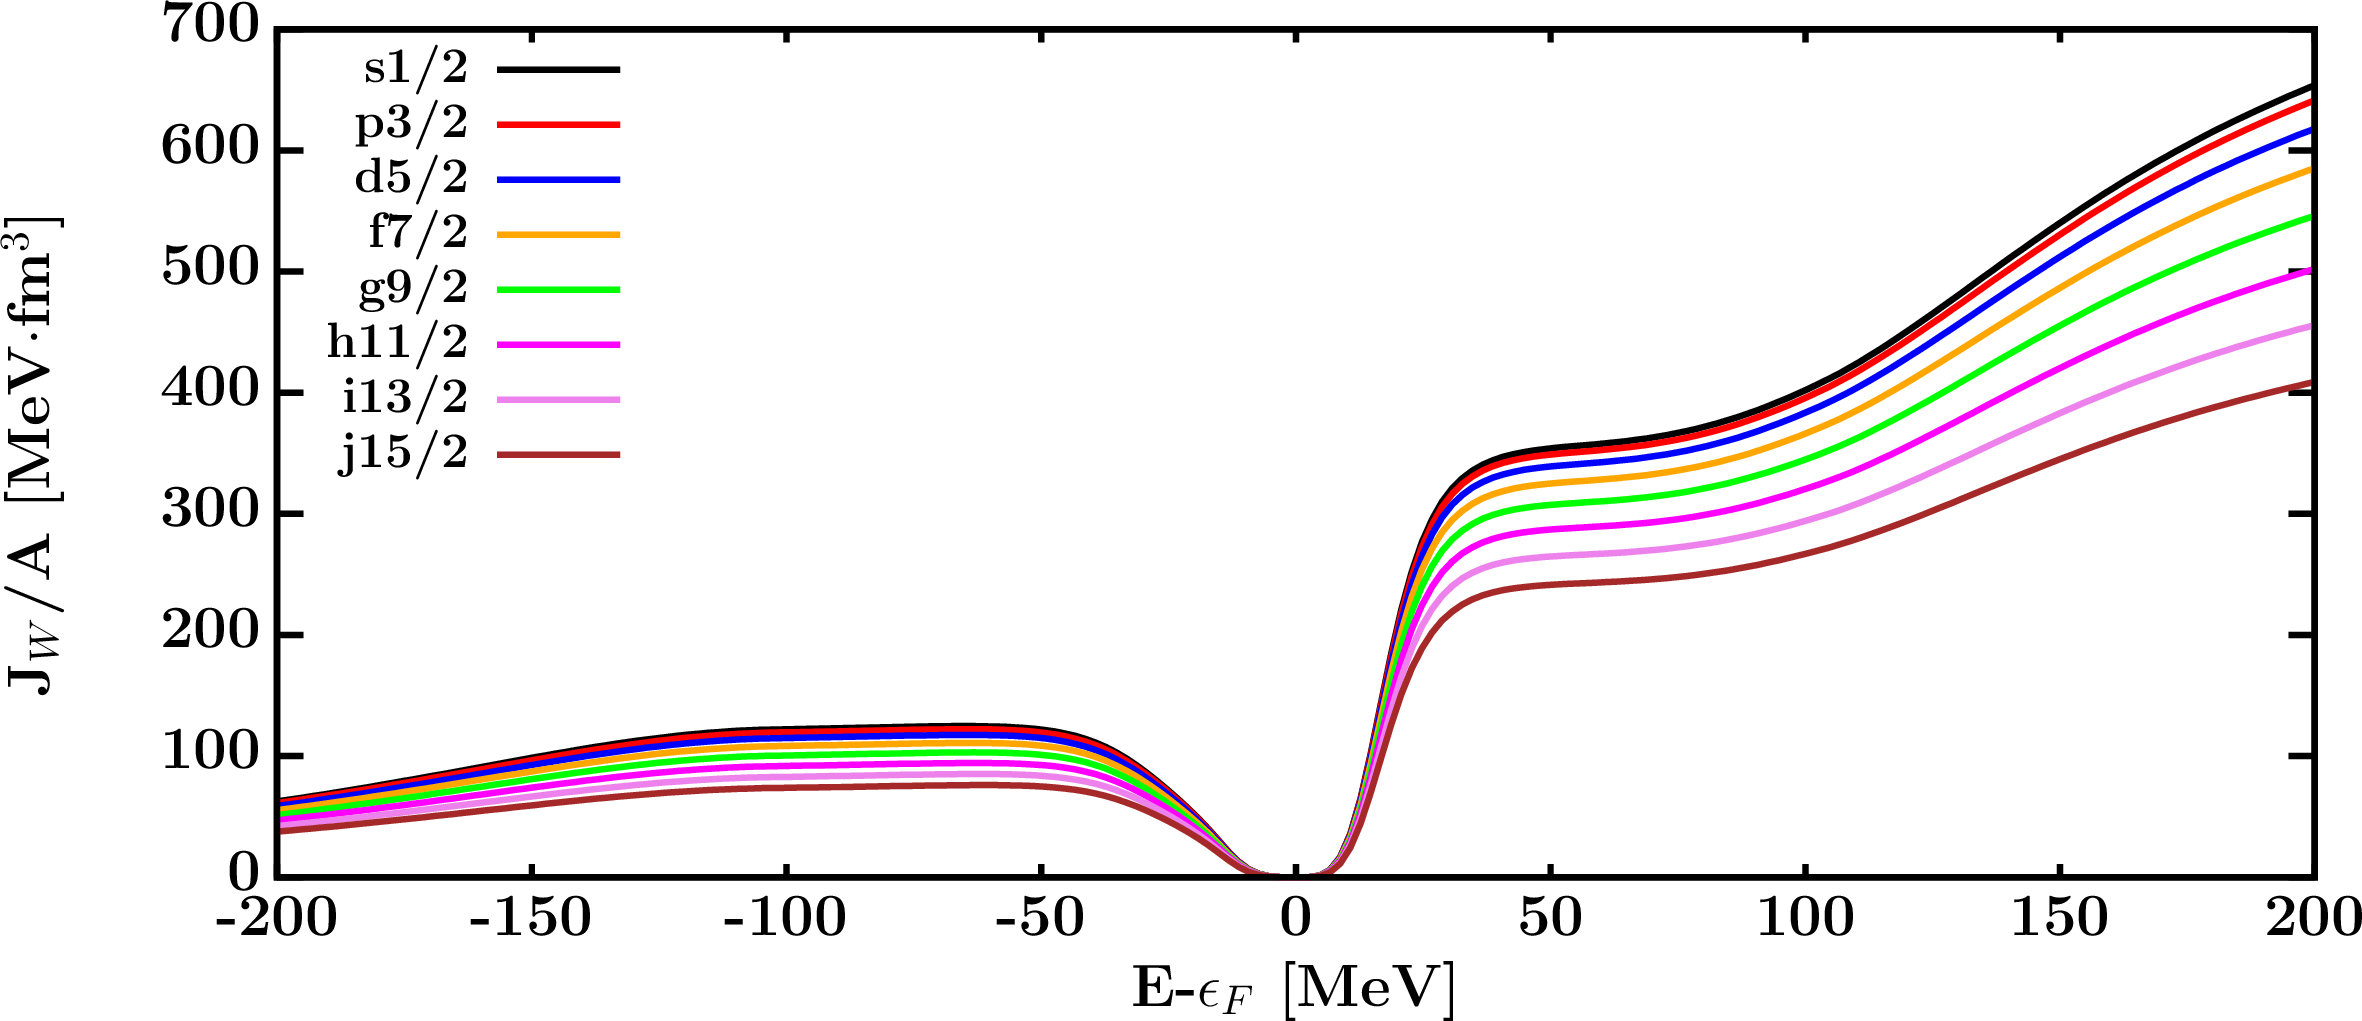
\includegraphics[width=\linewidth]{figures/ca40_protonVolumeIntegrals.png}
%        \caption{\caForty\ proton volume integral}
%        \label{DOMFitData_ca40_proton_potentialIntegral}
%    \end{subfigure}\hspace{6pt}
%    \begin{subfigure}[b]{0.45\textwidth}
%        \centering
%        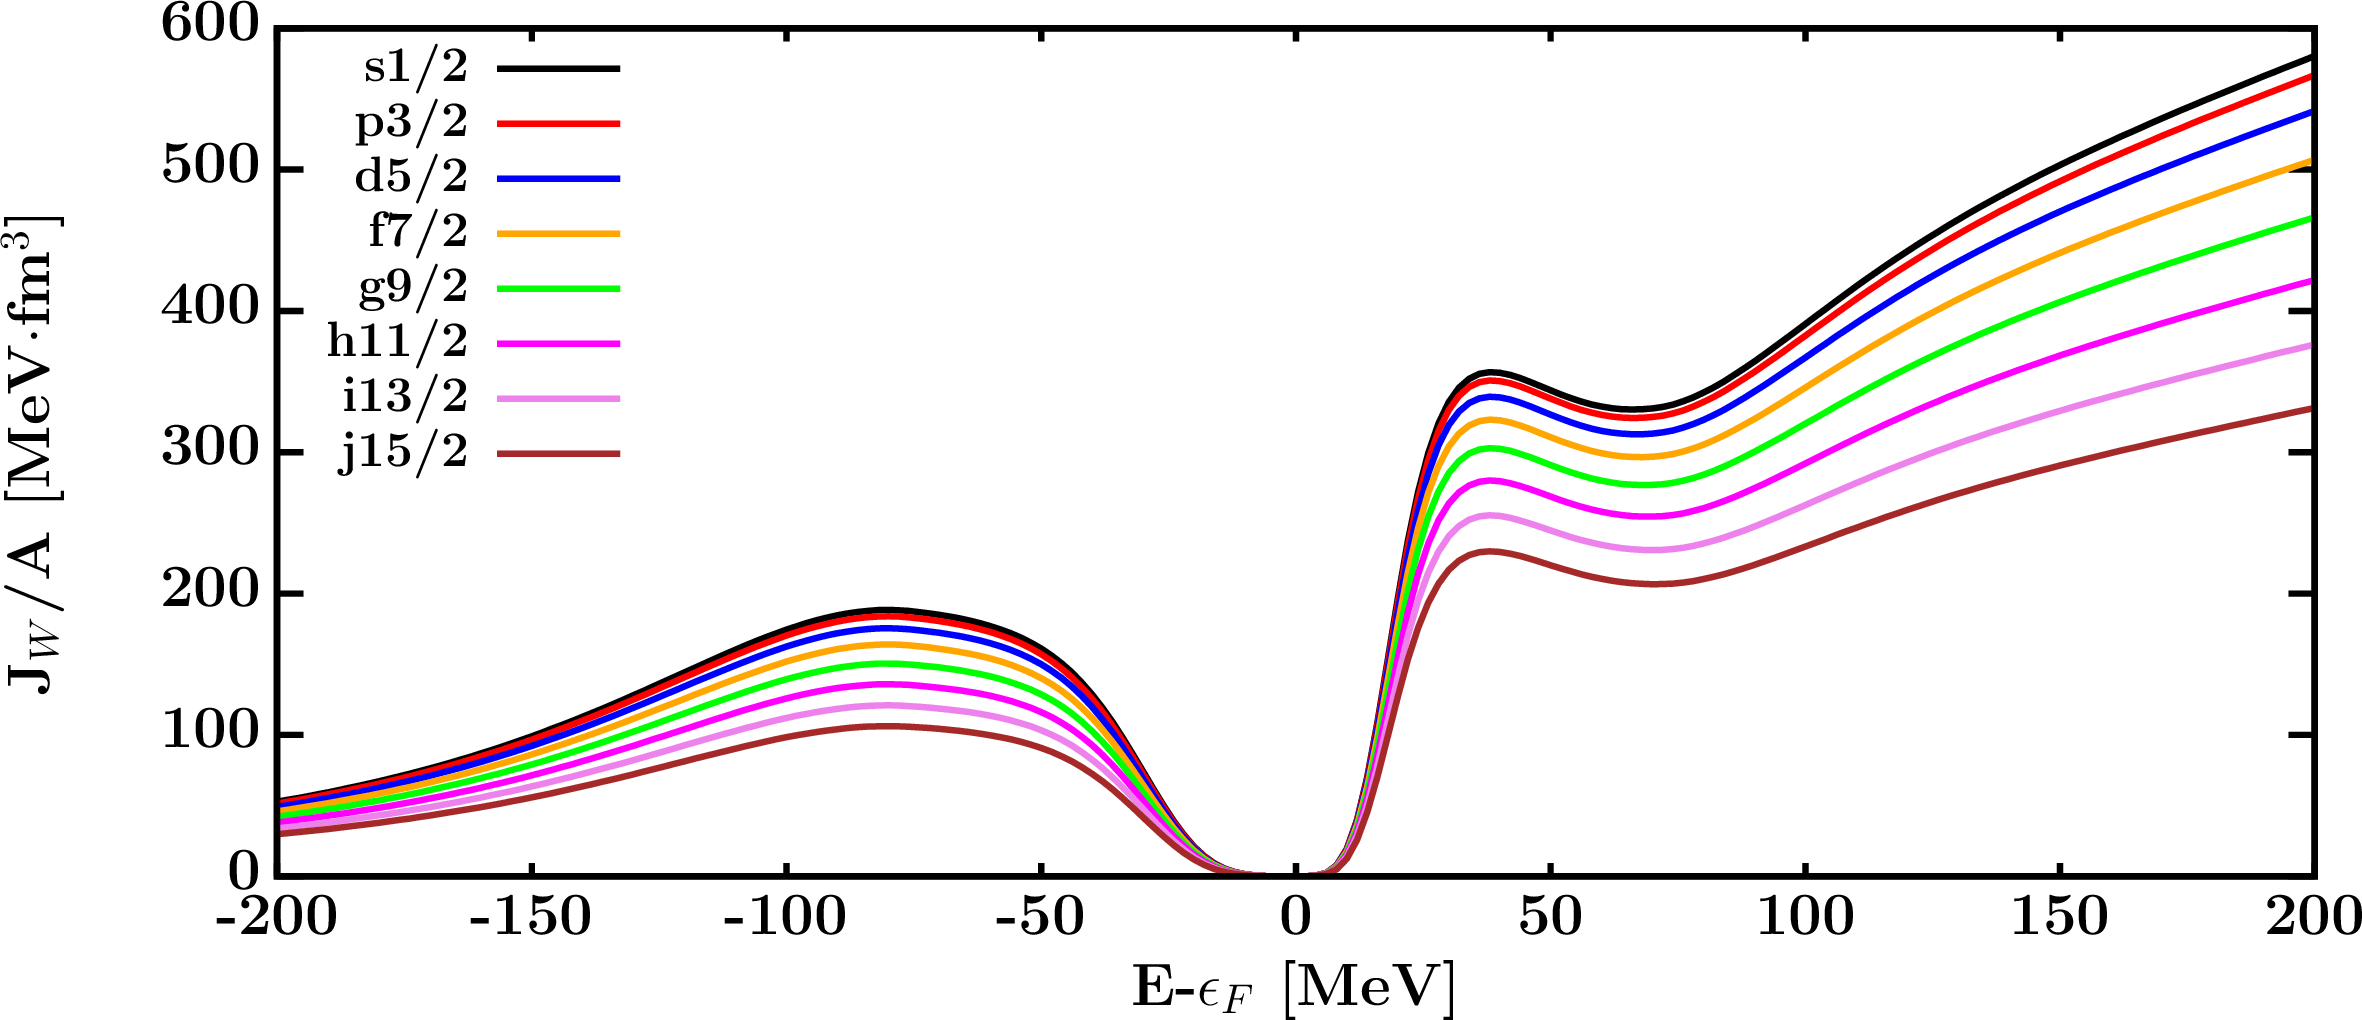
\includegraphics[width=\linewidth]{figures/ca40_neutronVolumeIntegrals.png}
%        \caption{\caForty\ neutron volume integral}
%        \label{DOMFitData_ca40_neutron_potentialIntegral}
%    \end{subfigure}\vspace{0.3in}
%    \begin{subfigure}[b]{0.45\textwidth}
%        \centering
%        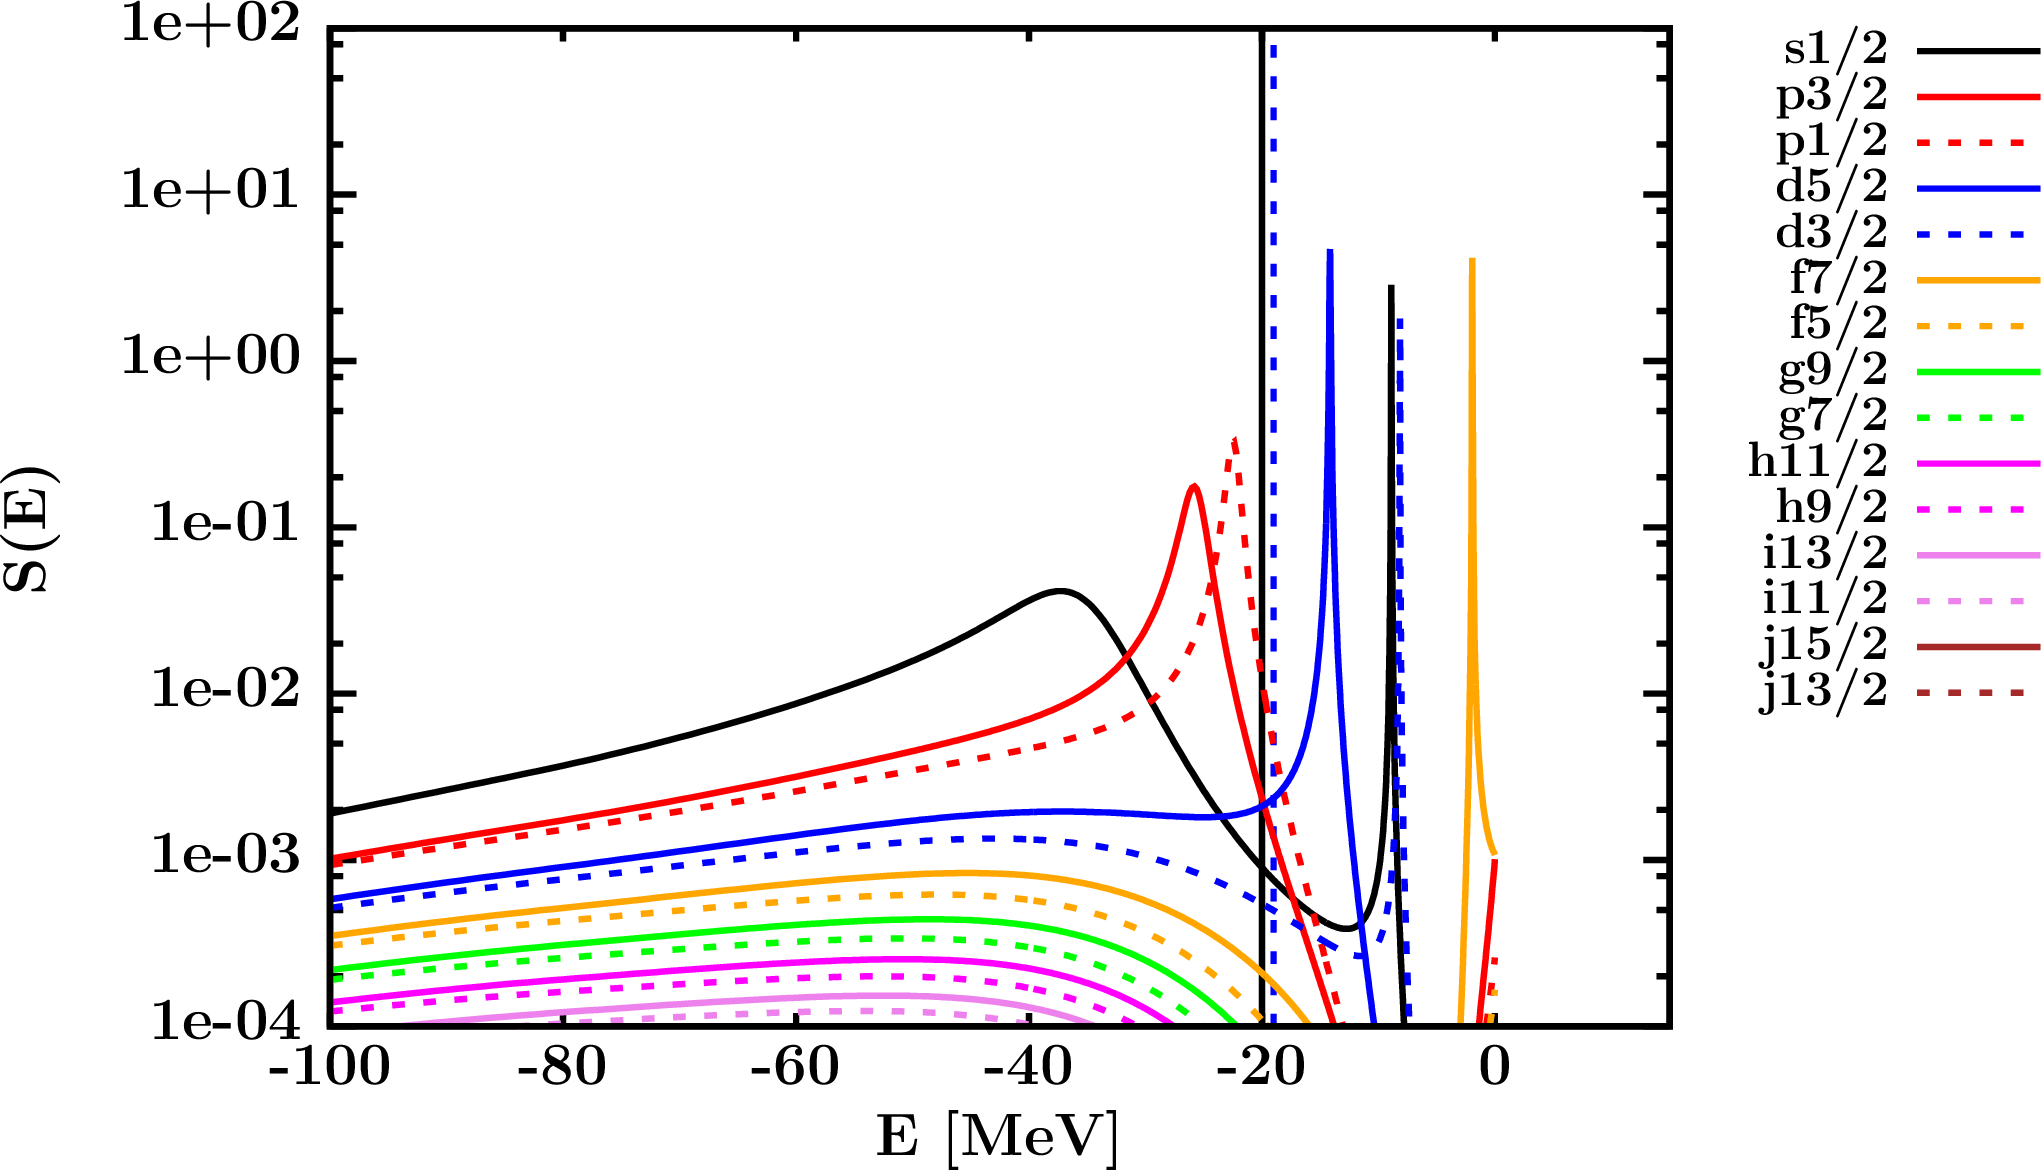
\includegraphics[width=\linewidth]{figures/ca40_protonSpectralFunctions.png}
%        \caption{\caForty\ proton spectral functions}
%        \label{DOMFitData_ca40_proton_spectralFunctions}
%    \end{subfigure}\hspace{6pt}
%    \begin{subfigure}[b]{0.45\textwidth}
%        \centering
%        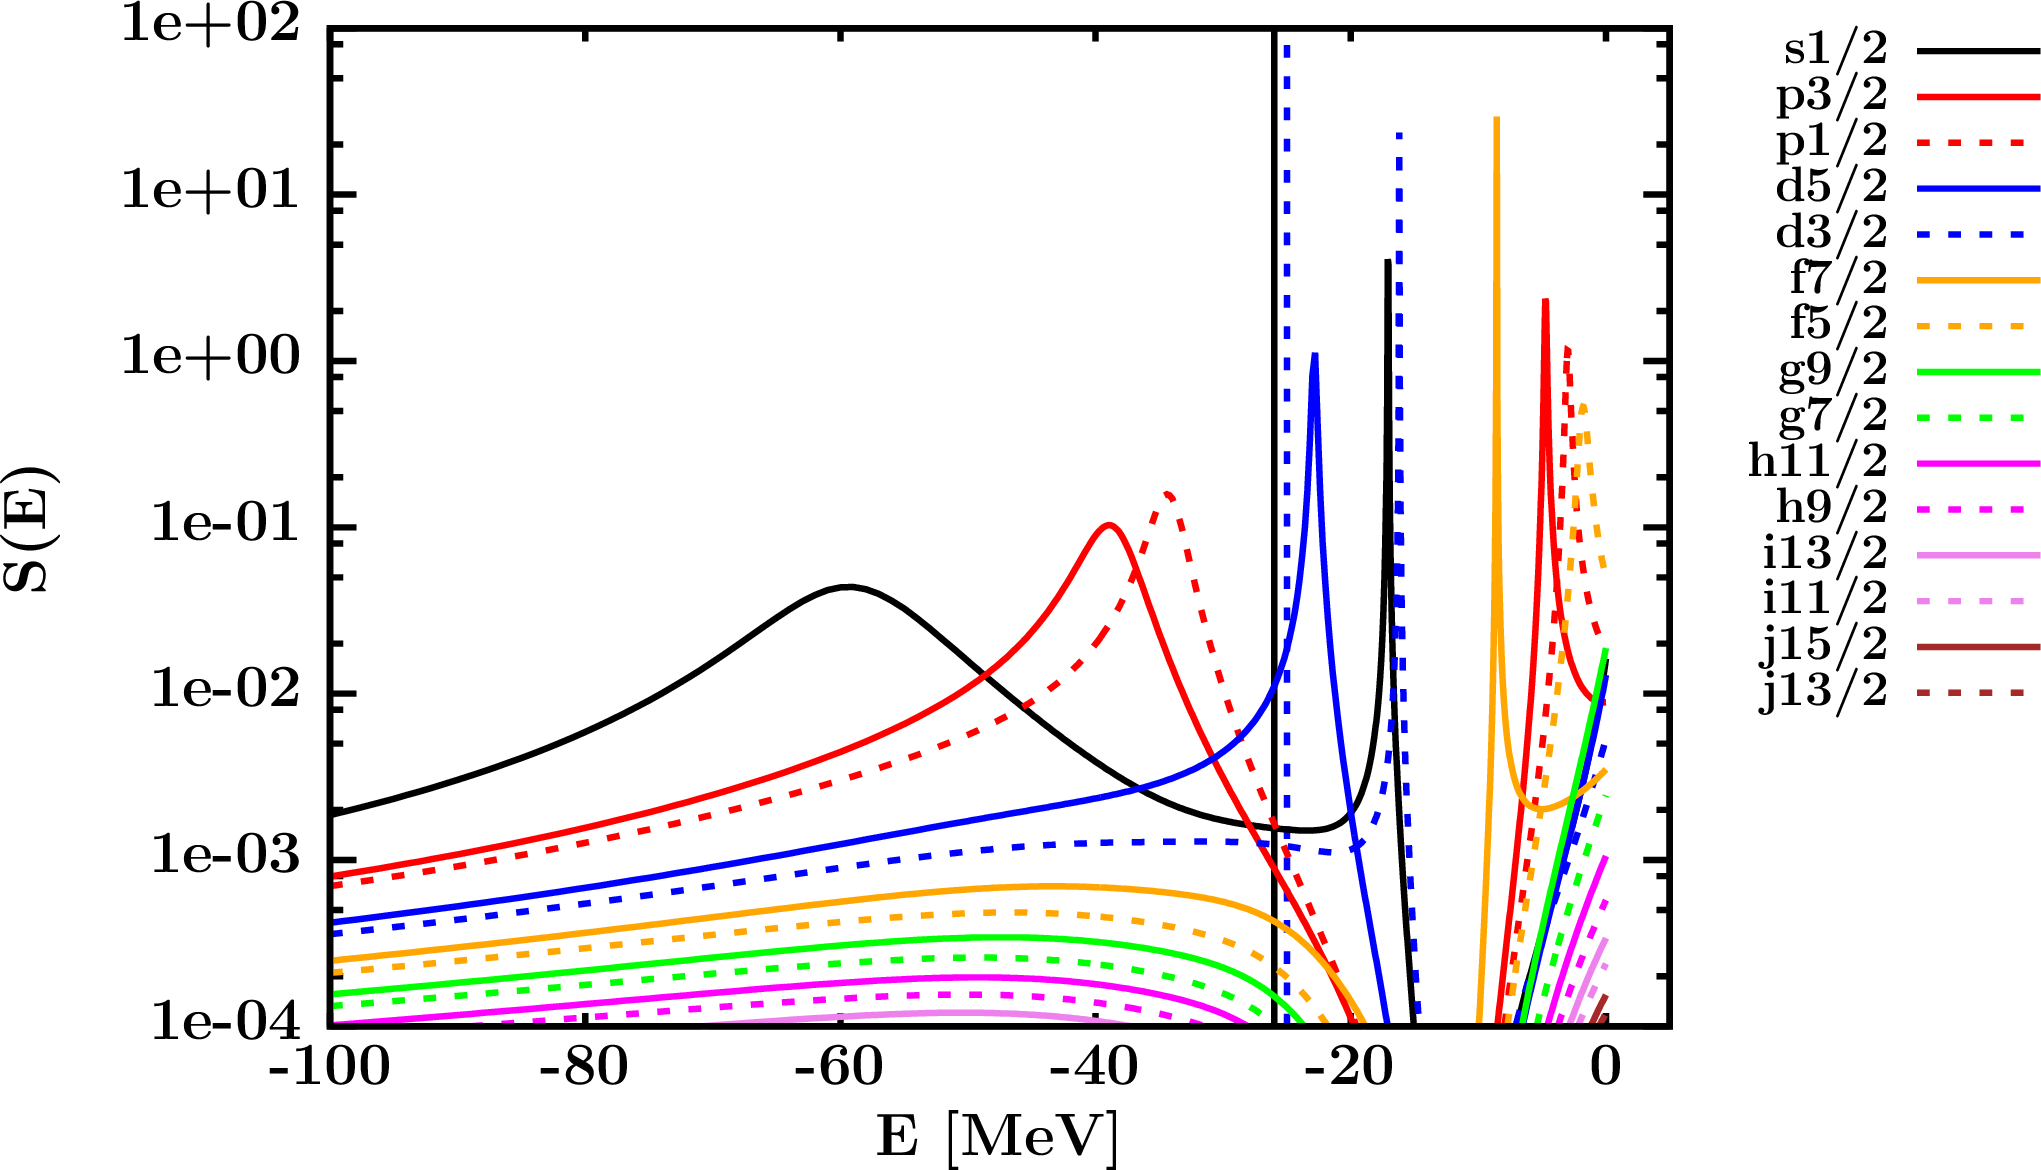
\includegraphics[width=\linewidth]{figures/ca40_neutronSpectralFunctions.png}
%        \caption{\caForty\ neutron spectral functions}
%        \label{DOMFitData_ca40_neutron_spectralFunctions}
%    \end{subfigure}
%\end{figure}
%\afterpage{\clearpage}
%\begin{figure}[hbtp]
%    \captionsetup[subfigure]{labelformat=empty}
%    \centering
%    \begin{subfigure}[b]{0.45\textwidth}
%        \centering
%        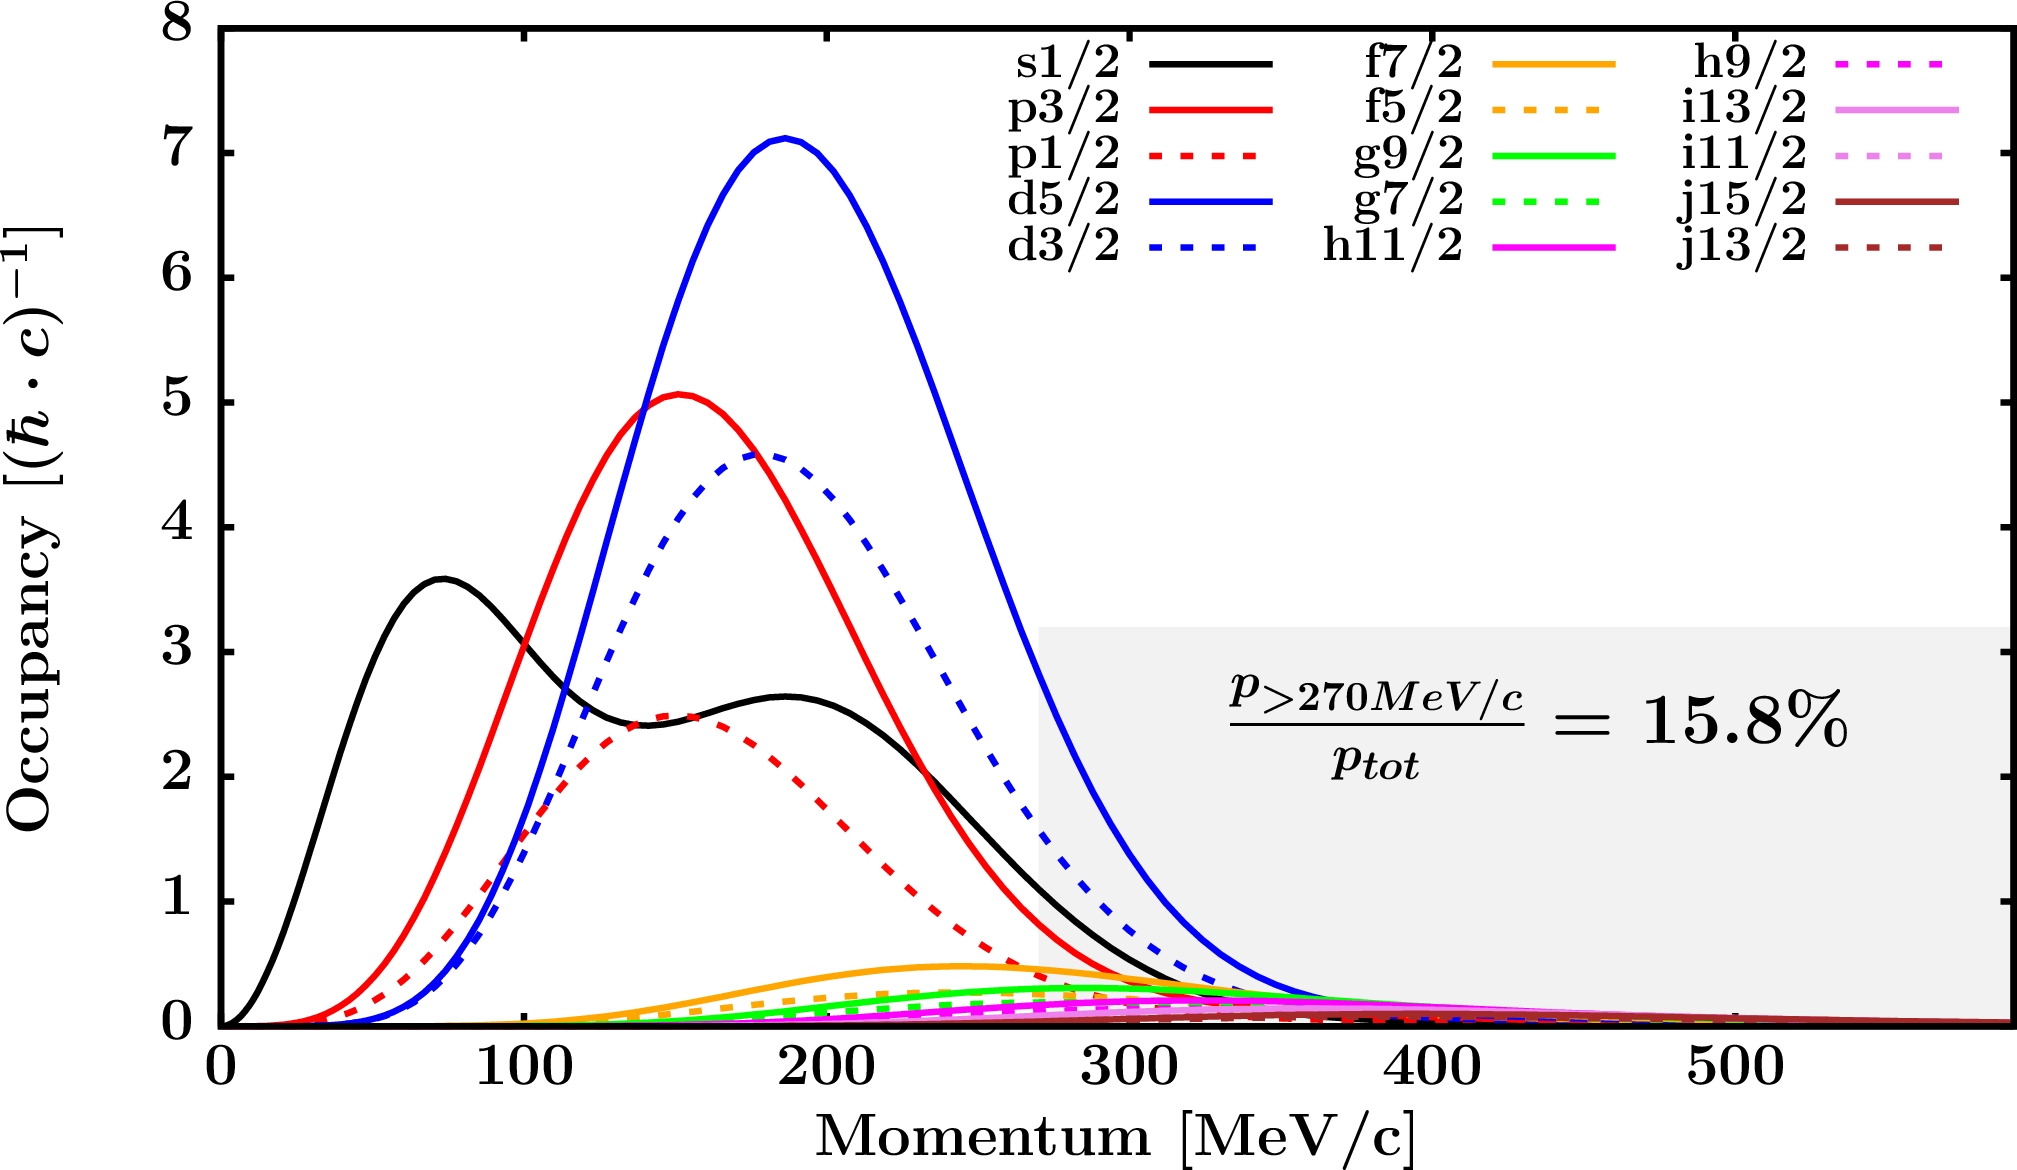
\includegraphics[width=\linewidth]{figures/ca40_protonLJMomentumDistIntegral.png}
%        \caption{\caForty\ proton momentum distribution}
%        \label{DOMFitData_ca40_proton_momentumDist}
%    \end{subfigure}\hspace{6pt}
%    \begin{subfigure}[b]{0.45\textwidth}
%        \centering
%        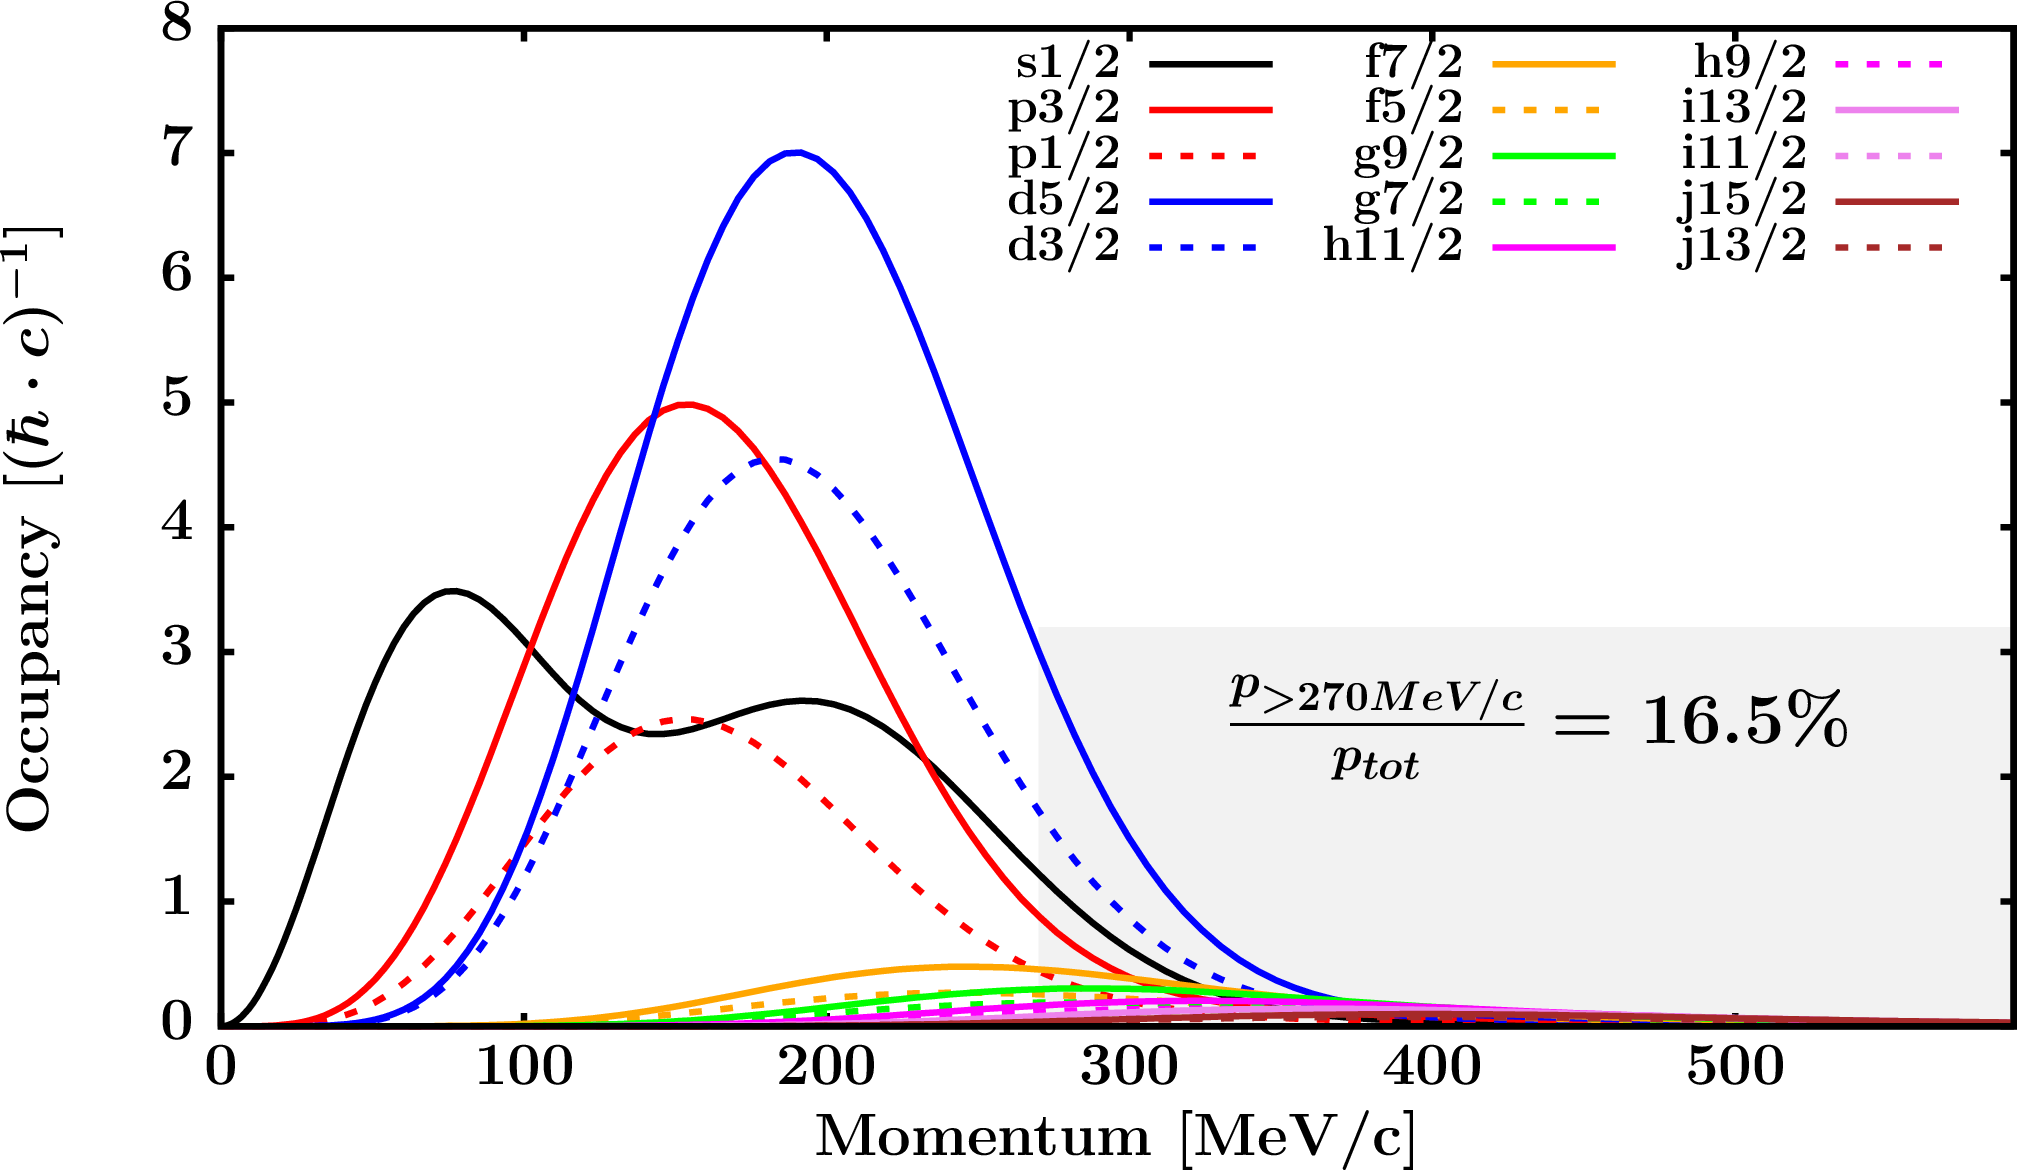
\includegraphics[width=\linewidth]{figures/ca40_neutronLJMomentumDistIntegral.png}
%        \caption{\caForty\ neutron momentum distribution}
%        \label{DOMFitData_ca40_neutron_momentumDist}
%    \end{subfigure}\vspace{0.3in}
%    \begin{subfigure}{0.45\textwidth}
%        \centering
%        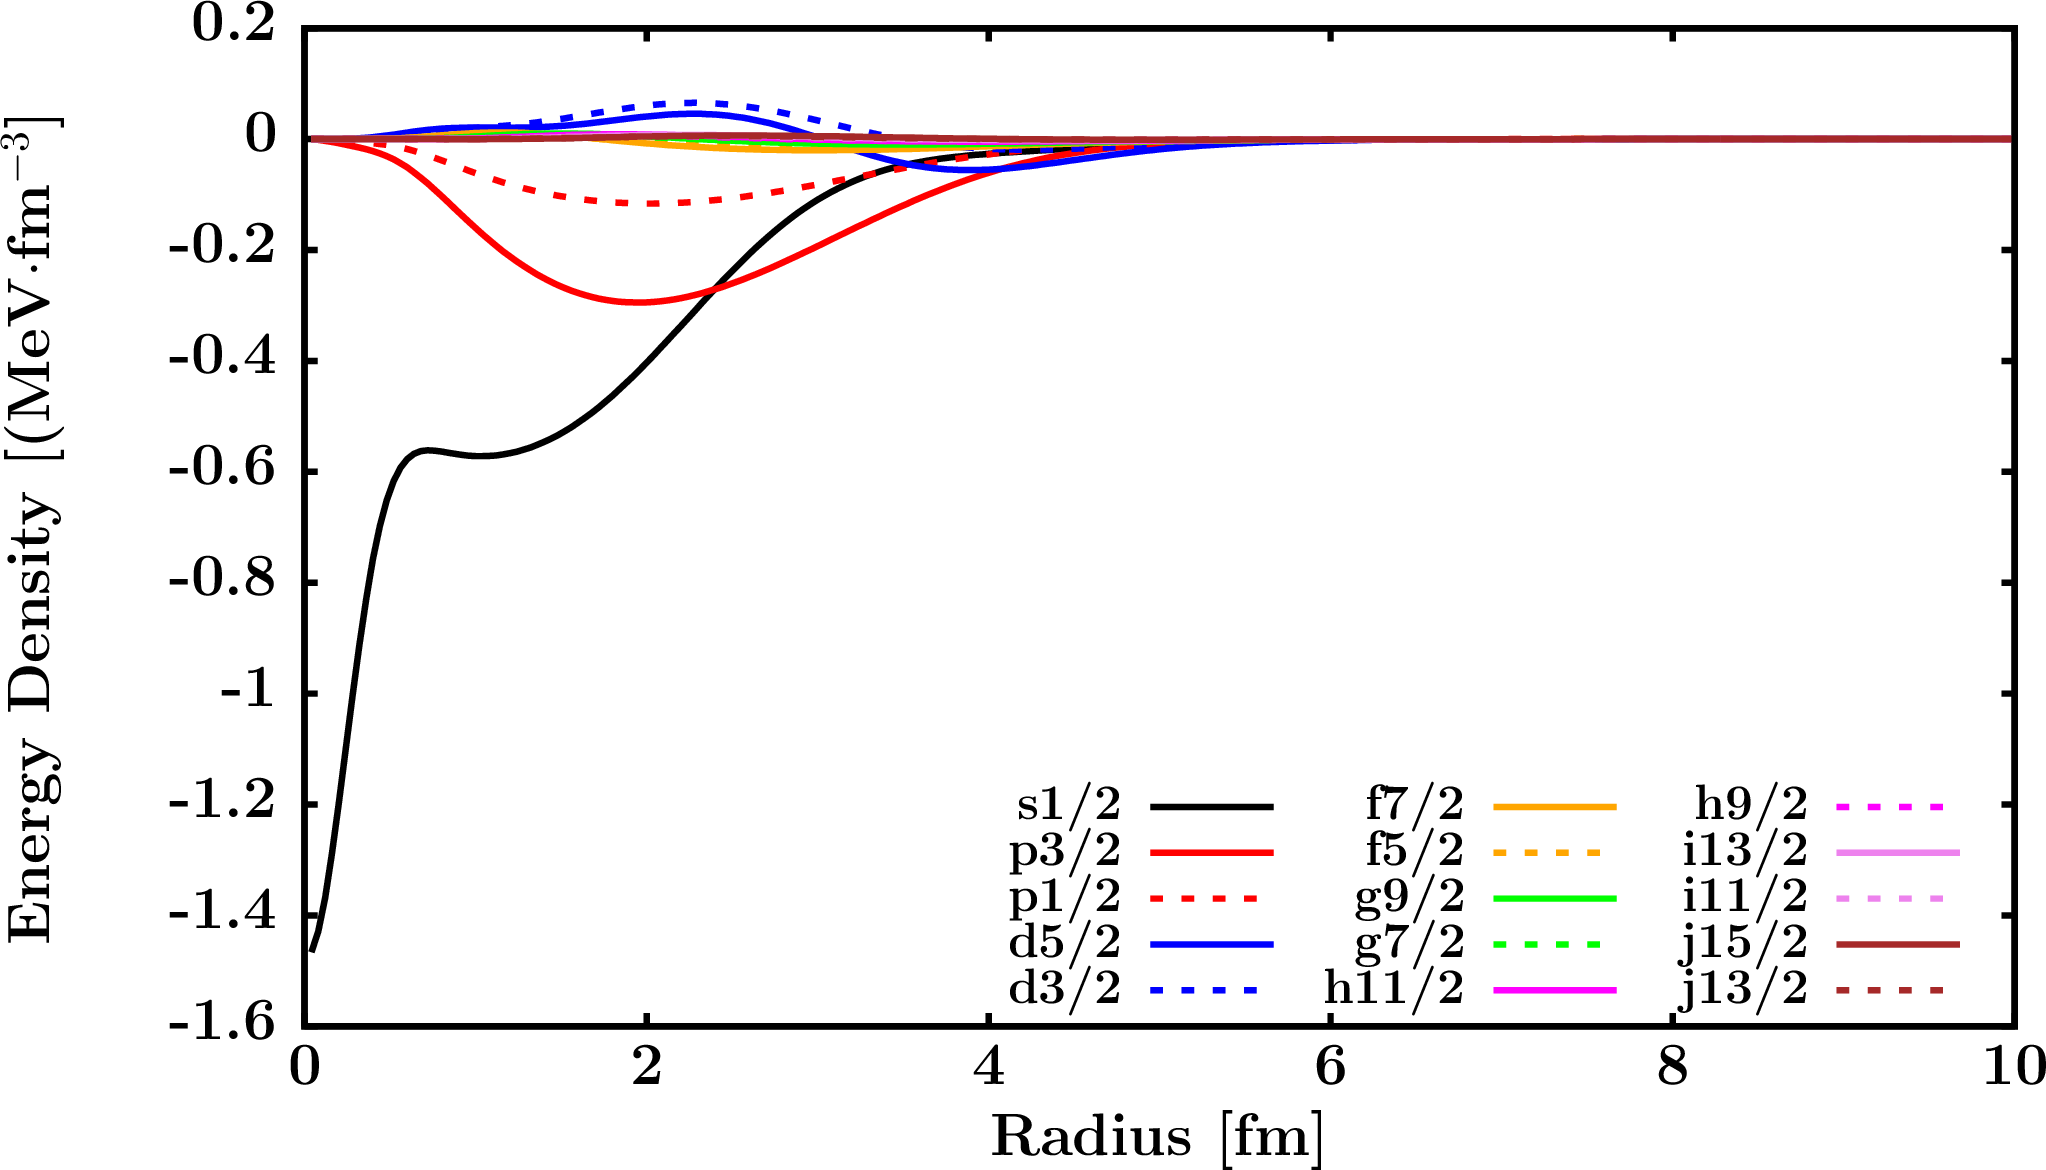
\includegraphics[width=\linewidth]{figures/ca40_EnergyDist.png}
%        \caption{\caForty\ energy distribution by LJ}
%        \label{DOMFitData_ca40_proton_energyDistInt}
%    \end{subfigure}\hspace{6pt}
%    \begin{subfigure}{0.45\textwidth}
%        \centering
%        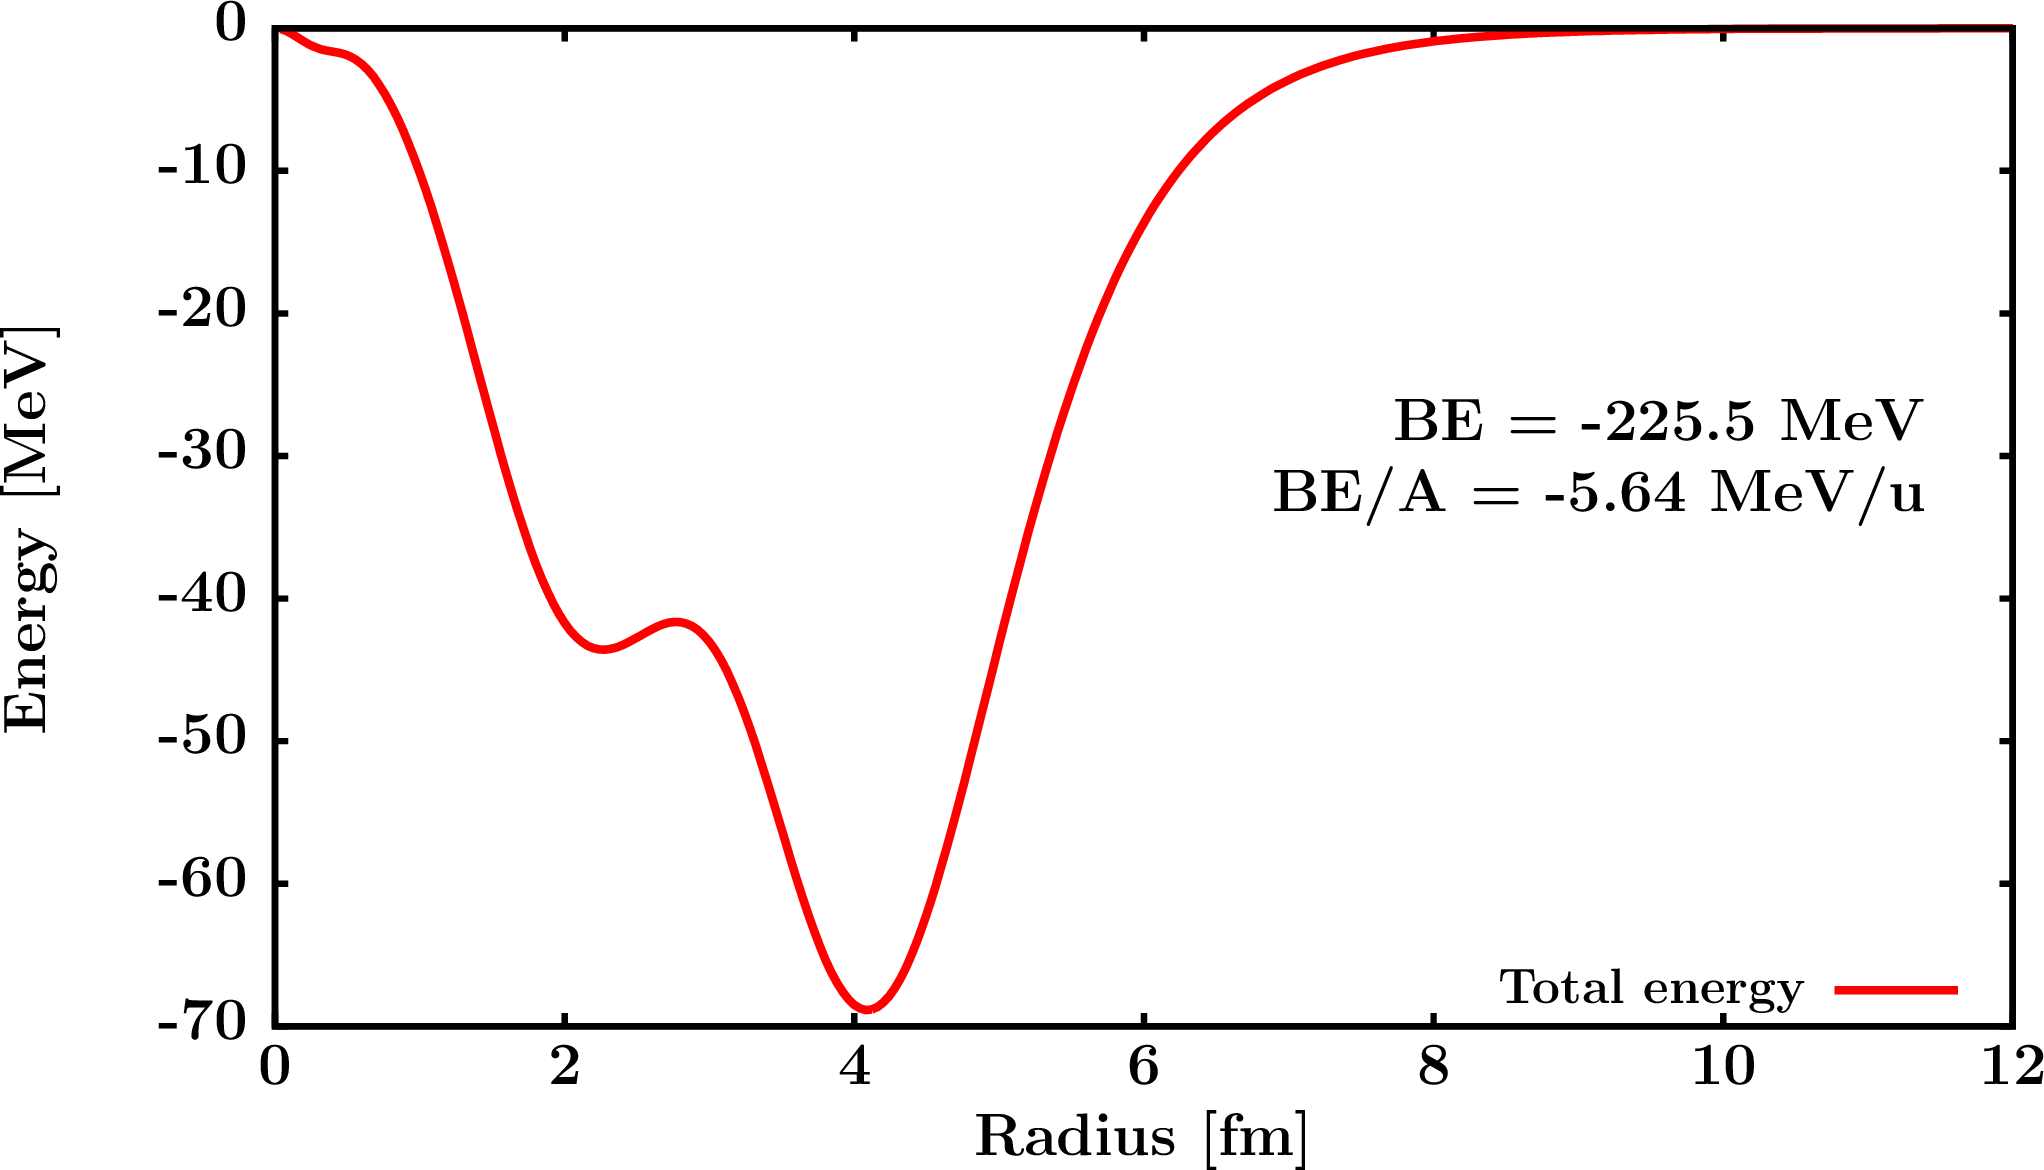
\includegraphics[width=\linewidth]{figures/ca40_EnergyDistIntegral.png}
%        \caption{\caForty\ energy distribution integral}
%        \label{DOMFitData_ca40_neutron_energyDistInt}
%    \end{subfigure}\vspace{0.4in}
%    \begin{subfigure}{0.70\textwidth}
%        \centering
%        \includegraphics[width=\linewidth]{figures/ca40_matterDensity.png}
%        \caption{\caForty\ matter density distribution}
%        \label{DOMFitData_ca40_matterDensity}
%    \end{subfigure}
%\end{figure}
%
%\newpage
%\section{DOM fit of \caEight}
%\label{ca48DOMOutput}
%\begin{figure}[hbtp]
%    \captionsetup[subfigure]{labelformat=empty}
%    \centering
%    \begin{subfigure}[c]{0.39\textheight}
%        \centering
%        \includegraphics[width=\linewidth]{figures/ca48_protonElastic.png}
%        \caption{\caEight\ proton elastic scattering}
%        \label{DOMFitData_ca48_proton_elastic}
%    \end{subfigure}\hspace{6pt}
%    \begin{subfigure}[c]{0.39\textheight}
%        \centering
%        \includegraphics[width=0.52\linewidth]{figures/ca48_neutronElastic.png}
%        \caption{\caEight\ neutron elastic scattering}
%        \label{DOMFitData_ca48_neutron_elastic}
%    \end{subfigure}\vspace{0.70in}
%    \begin{subfigure}[c]{0.45\textwidth}
%        \centering
%        %\includegraphics[width=\linewidth]{figures/ca48_protonInelastic.png}
%        \caption{No \caEight\ proton \rxn\\ data were available}
%        \label{DOMFitData_ca48_proton_inelastic}
%    \end{subfigure}\hspace{6pt}
%    \begin{subfigure}[c]{0.45\textwidth}
%        \centering
%        \includegraphics[width=\linewidth]{figures/ca48_neutronInelastic.png}
%        \caption{\caEight\ neutron \rxn\ and \tot}
%        \label{DOMFitData_ca48_neutron_inelastic}
%    \end{subfigure}
%\end{figure}
%\afterpage{\clearpage}
%\begin{figure}[hbtp]
%    \captionsetup[subfigure]{labelformat=empty}
%    \centering
%    \begin{subfigure}[b]{0.45\textwidth}
%        \centering
%        \includegraphics[width=\linewidth]{figures/ca48_chargeDensity.png}
%        \caption{\caEight\ charge density}
%        \label{DOMFitData_ca48_chargeDensity}
%    \end{subfigure}\hspace{6pt}
%    \begin{subfigure}[b]{0.45\textwidth}
%        \centering
%        \includegraphics[width=\linewidth]{figures/ca48_SPLevels.png}
%        \caption{\caEight\ single-particle levels}
%        \label{DOMFitData_ca48_SPLevels}
%    \end{subfigure}\vspace{0.3in}
%    \begin{subfigure}[b]{0.45\textwidth}
%        \centering
%        \includegraphics[width=\linewidth]{figures/ca48_protonPotentials.png}
%        \caption{\caEight\ proton potential energy-dependence}
%        \label{DOMFitData_ca48_proton_potentialComponent_energy}
%    \end{subfigure}\hspace{6pt}
%    \begin{subfigure}[b]{0.45\linewidth}
%        \centering
%        \includegraphics[width=\linewidth]{figures/ca48_neutronPotentials.png}
%        \caption{\caEight\ neutron potential energy-dependence}
%        \label{DOMFitData_ca48_neutron_potentialComponent_energy}
%    \end{subfigure}\vspace{0.3in}
%    \begin{subfigure}[b]{0.45\textwidth}
%        \centering
%        \includegraphics[width=\linewidth]{figures/ca48_protonVolumeIntegrals.png}
%        \caption{\caEight\ proton volume integral}
%        \label{DOMFitData_ca48_proton_potentialIntegral}
%    \end{subfigure}\hspace{6pt}
%    \begin{subfigure}[b]{0.45\textwidth}
%        \centering
%        \includegraphics[width=\linewidth]{figures/ca48_neutronVolumeIntegrals.png}
%        \caption{\caEight\ neutron volume integral}
%        \label{DOMFitData_ca48_neutron_potentialIntegral}
%    \end{subfigure}\vspace{0.3in}
%    \begin{subfigure}[b]{0.45\textwidth}
%        \centering
%        \includegraphics[width=\linewidth]{figures/ca48_protonSpectralFunctions.png}
%        \caption{\caEight\ proton spectral functions}
%        \label{DOMFitData_ca48_proton_spectralFunctions}
%    \end{subfigure}\hspace{6pt}
%    \begin{subfigure}[b]{0.45\textwidth}
%        \centering
%        \includegraphics[width=\linewidth]{figures/ca48_neutronSpectralFunctions.png}
%        \caption{\caEight\ neutron spectral functions}
%        \label{DOMFitData_ca48_neutron_spectralFunctions}
%    \end{subfigure}
%\end{figure}
%\afterpage{\clearpage}
%\begin{figure}[hbtp]
%    \captionsetup[subfigure]{labelformat=empty}
%    \centering
%    \begin{subfigure}[b]{0.45\textwidth}
%        \centering
%        \includegraphics[width=\linewidth]{figures/ca48_protonLJMomentumDistIntegral.png}
%        \caption{\caEight\ proton momentum distribution}
%        \label{DOMFitData_ca48_proton_momentumDist}
%    \end{subfigure}\hspace{6pt}
%    \begin{subfigure}[b]{0.45\textwidth}
%        \centering
%        \includegraphics[width=\linewidth]{figures/ca48_neutronLJMomentumDistIntegral.png}
%        \caption{\caEight\ neutron momentum distribution}
%        \label{DOMFitData_ca48_neutron_momentumDist}
%    \end{subfigure}\vspace{0.3in}
%    \begin{subfigure}{0.45\textwidth}
%        \centering
%        \includegraphics[width=\linewidth]{figures/ca48_EnergyDist.png}
%        \caption{\caEight\ energy distribution by LJ}
%        \label{DOMFitData_ca48_proton_energyDistInt}
%    \end{subfigure}\hspace{6pt}
%    \begin{subfigure}{0.45\textwidth}
%        \centering
%        \includegraphics[width=\linewidth]{figures/ca48_EnergyDistIntegral.png}
%        \caption{\caEight\ energy distribution integral}
%        \label{DOMFitData_ca48_neutron_energyDistInt}
%    \end{subfigure}\vspace{0.4in}
%    \begin{subfigure}{0.70\textwidth}
%        \centering
%        \includegraphics[width=\linewidth]{figures/ca48_matterDensity.png}
%        \caption{\caEight\ matter density distribution}
%        \label{DOMFitData_ca48_matterDensity}
%    \end{subfigure}
%\end{figure}
%
%\section{DOM fit of \niEight}
%
%\label{ni58DOMOutput}
%\begin{figure}[H]
%    \centering
%    \begin{minipage}{0.45\textwidth}
%        \centering
%        \includegraphics[width=1.0\textwidth]{figures/ni58_protonElastic.png}
%        \caption{\niEight\ proton elastic scattering data}
%        \label{DOMFitData_ni58_proton_elastic}
%    \end{minipage}\hfill
%    \begin{minipage}{0.45\textwidth}
%        \centering
%        \includegraphics[width=1.0\textwidth]{figures/ni58_neutronElastic.png}
%        \caption{\niEight\ neutron elastic scattering data}
%        \label{DOMFitData_ni58_neutron_elastic}
%    \end{minipage}
%\end{figure}
%
%\begin{figure}[H]
%    \centering
%    \begin{minipage}{0.45\textwidth}
%        \centering
%        \includegraphics[width=1.0\textwidth]{figures/ni58_protonInelastic.png}
%        \caption{\niEight\ proton \rxn data}
%        \label{DOMFitData_ni58_proton_inelastic}
%    \end{minipage}\hfill
%    \begin{minipage}{0.45\textwidth}
%        \centering
%        \includegraphics[width=1.0\textwidth]{figures/ni58_neutronInelastic.png}
%        \caption{\niEight\ neutron \rxn and \tot data}
%        \label{DOMFitData_ni58_neutron_inelastic}
%    \end{minipage}
%\end{figure}
%
%\afterpage{\clearpage}
%
%\begin{figure}[H]
%    \centering
%    \begin{minipage}{0.45\textwidth}
%        \centering
%        \includegraphics[width=1.0\textwidth]{figures/ni58_chargeDensity.png}
%        \caption{\niEight\ charge density data}
%        \label{DOMFitData_ni58_chargeDensity}
%    \end{minipage}\hfill
%    \begin{minipage}{0.45\textwidth}
%        \centering
%        \includegraphics[width=1.0\textwidth]{figures/ni58_SPLevels.png}
%        \caption{\niEight\ single-particle levels}
%        \label{DOMFitData_ni58_SPLevels}
%    \end{minipage}
%\end{figure}
%
%\afterpage{\clearpage}
%
%\begin{figure}[H]
%    \centering
%    \begin{minipage}{0.45\textwidth}
%        \centering
%        \includegraphics[width=1.0\textwidth]{figures/ni58_protonPotentials.png}
%        \caption{\niEight\ proton potential energy-dependence}
%        \label{DOMFitData_ni58_proton_potentialComponent_energy}
%    \end{minipage}\hfill
%    \begin{minipage}{0.45\textwidth}
%        \centering
%        \includegraphics[width=1.0\textwidth]{figures/ni58_neutronPotentials.png}
%        \caption{\niEight\ proton potential energy-dependence}
%        \label{DOMFitData_ni58_neutron_potentialComponent_energy}
%    \end{minipage}
%\end{figure}
%
%\begin{figure}[H]
%    \centering
%    \begin{minipage}{0.45\textwidth}
%        \centering
%        \includegraphics[width=1.0\textwidth]{figures/ni58_protonVolumeIntegrals.png}
%        \caption{\niEight\ proton potential, integrated over r-space}
%        \label{DOMFitData_ni58_proton_potentialIntegral}
%    \end{minipage}\hfill
%    \begin{minipage}{0.45\textwidth}
%        \centering
%        \includegraphics[width=1.0\textwidth]{figures/ni58_neutronVolumeIntegrals.png}
%        \caption{\niEight\ neutron potential, integrated over r-space}
%        \label{DOMFitData_ni58_neutron_potentialIntegral}
%    \end{minipage}
%\end{figure}
%
%\afterpage{\clearpage}
%
%\begin{figure}[H]
%    \centering
%    \begin{minipage}{0.45\textwidth}
%        \centering
%        \includegraphics[width=1.0\textwidth]{figures/ni58_protonSpectralFunctions.png}
%        \caption{\niEight\ proton spectral functions}
%        \label{DOMFitData_ni58_proton_spectralFunctions}
%    \end{minipage}\hfill
%    \begin{minipage}{0.45\textwidth}
%        \centering
%        \includegraphics[width=1.0\textwidth]{figures/ni58_neutronSpectralFunctions.png}
%        \caption{\niEight\ neutron spectral functions}
%        \label{DOMFitData_ni58_neutron_spectralFunctions}
%    \end{minipage}
%\end{figure}
%
%\begin{figure}[H]
%    \centering
%    \includegraphics[width = 0.5\textwidth]{figures/ni58_matterDensity.png}
%    \caption{\niEight\ matter density distribution}
%    \label{DOMFitData_ni58_matterDensity}
%\end{figure}
%
%\begin{figure}[H]
%    \centering
%    \includegraphics[width = 0.5\textwidth]{figures/ni58_momentumDistribution.png}
%    \caption{\niEight\ momentum distribution}
%    \label{DOMFitData_ni58_momentumDistribution}
%\end{figure}
%
%\begin{figure}[H]
%    \centering
%    \includegraphics[width = 0.5\textwidth]{figures/ni58_energyDensity.png}
%    \caption{\niEight\ energy density distribution}
%    \label{DOMFitData_ni58_energyDensity}
%\end{figure}
%
%\section{DOM fit of \niFour}
%
%\label{ni64DOMOutput}
%\begin{figure}[H]
%    \centering
%    \begin{minipage}{0.45\textwidth}
%        \centering
%        \includegraphics[width=1.0\textwidth]{figures/ni64_protonElastic.png}
%        \caption{\niFour\ proton elastic scattering data}
%        \label{DOMFitData_ni64_proton_elastic}
%    \end{minipage}\hfill
%    \begin{minipage}{0.45\textwidth}
%        \centering
%        \includegraphics[width=1.0\textwidth]{figures/ni64_neutronElastic.png}
%        \caption{\niFour\ neutron elastic scattering data}
%        \label{DOMFitData_ni64_neutron_elastic}
%    \end{minipage}
%\end{figure}
%
%\begin{figure}[H]
%    \centering
%    \begin{minipage}{0.45\textwidth}
%        \centering
%        \includegraphics[width=1.0\textwidth]{figures/ni64_protonInelastic.png}
%        \caption{\niFour\ proton \rxn data}
%        \label{DOMFitData_ni64_proton_inelastic}
%    \end{minipage}\hfill
%    \begin{minipage}{0.45\textwidth}
%        \centering
%        \includegraphics[width=1.0\textwidth]{figures/ni64_neutronInelastic.png}
%        \caption{\niFour\ neutron \rxn and \tot data}
%        \label{DOMFitData_ni64_neutron_inelastic}
%    \end{minipage}
%\end{figure}
%
%\afterpage{\clearpage}
%
%\begin{figure}[H]
%    \centering
%    \begin{minipage}{0.45\textwidth}
%        \centering
%        \includegraphics[width=1.0\textwidth]{figures/ni64_chargeDensity.png}
%        \caption{\niFour\ charge density data}
%        \label{DOMFitData_ni64_chargeDensity}
%    \end{minipage}\hfill
%    \begin{minipage}{0.45\textwidth}
%        \centering
%        \includegraphics[width=1.0\textwidth]{figures/ni64_SPLevels.png}
%        \caption{\niFour\ single-particle levels}
%        \label{DOMFitData_ni64_SPLevels}
%    \end{minipage}
%\end{figure}
%
%\afterpage{\clearpage}
%
%\begin{figure}[H]
%    \centering
%    \begin{minipage}{0.45\textwidth}
%        \centering
%        \includegraphics[width=1.0\textwidth]{figures/ni64_protonPotentials.png}
%        \caption{\niFour\ proton potential energy-dependence}
%        \label{DOMFitData_ni64_proton_potentialComponent_energy}
%    \end{minipage}\hfill
%    \begin{minipage}{0.45\textwidth}
%        \centering
%        \includegraphics[width=1.0\textwidth]{figures/ni64_neutronPotentials.png}
%        \caption{\niFour\ proton potential energy-dependence}
%        \label{DOMFitData_ni64_neutron_potentialComponent_energy}
%    \end{minipage}
%\end{figure}
%
%\begin{figure}[H]
%    \centering
%    \begin{minipage}{0.45\textwidth}
%        \centering
%        \includegraphics[width=1.0\textwidth]{figures/ni64_protonVolumeIntegrals.png}
%        \caption{\niFour\ proton potential, integrated over r-space}
%        \label{DOMFitData_ni64_proton_potentialIntegral}
%    \end{minipage}\hfill
%    \begin{minipage}{0.45\textwidth}
%        \centering
%        \includegraphics[width=1.0\textwidth]{figures/ni64_neutronVolumeIntegrals.png}
%        \caption{\niFour\ neutron potential, integrated over r-space}
%        \label{DOMFitData_ni64_neutron_potentialIntegral}
%    \end{minipage}
%\end{figure}
%
%\afterpage{\clearpage}
%
%\begin{figure}[H]
%    \centering
%    \begin{minipage}{0.45\textwidth}
%        \centering
%        \includegraphics[width=1.0\textwidth]{figures/ni64_protonSpectralFunctions.png}
%        \caption{\niFour\ proton spectral functions}
%        \label{DOMFitData_ni64_proton_spectralFunctions}
%    \end{minipage}\hfill
%    \begin{minipage}{0.45\textwidth}
%        \centering
%        \includegraphics[width=1.0\textwidth]{figures/ni64_neutronSpectralFunctions.png}
%        \caption{\niFour\ neutron spectral functions}
%        \label{DOMFitData_ni64_neutron_spectralFunctions}
%    \end{minipage}
%\end{figure}
%
%\begin{figure}[H]
%    \centering
%    \includegraphics[width = 0.5\textwidth]{figures/ni64_matterDensity.png}
%    \caption{\niFour\ matter density distribution}
%    \label{DOMFitData_ni64_matterDensity}
%\end{figure}
%
%\begin{figure}[H]
%    \centering
%    \includegraphics[width = 0.5\textwidth]{figures/ni64_momentumDistribution.png}
%    \caption{\niFour\ momentum distribution}
%    \label{DOMFitData_ni64_momentumDistribution}
%\end{figure}
%
%\begin{figure}[H]
%    \centering
%    \includegraphics[width = 0.5\textwidth]{figures/ni64_energyDensity.png}
%    \caption{\niFour\ energy density distribution}
%    \label{DOMFitData_ni64_energyDensity}
%\end{figure}
%
%\section{DOM fit of \snTwelve}
%
%\label{sn112DOMOutput}
%\begin{figure}[H]
%    \centering
%    \begin{minipage}{0.45\textwidth}
%        \centering
%        \includegraphics[width=1.0\textwidth]{figures/sn112_protonElastic.png}
%        \caption{\snTwelve\ proton elastic scattering data}
%        \label{DOMFitData_sn112_proton_elastic}
%    \end{minipage}\hfill
%    \begin{minipage}{0.45\textwidth}
%        \centering
%        \includegraphics[width=1.0\textwidth]{figures/sn112_neutronElastic.png}
%        \caption{\snTwelve\ neutron elastic scattering data}
%        \label{DOMFitData_sn112_neutron_elastic}
%    \end{minipage}
%\end{figure}
%
%\begin{figure}[H]
%    \centering
%    \begin{minipage}{0.45\textwidth}
%        \centering
%        \includegraphics[width=1.0\textwidth]{figures/sn112_protonInelastic.png}
%        \caption{\snTwelve\ proton \rxn data}
%        \label{DOMFitData_sn112_proton_inelastic}
%    \end{minipage}\hfill
%    \begin{minipage}{0.45\textwidth}
%        \centering
%        \includegraphics[width=1.0\textwidth]{figures/sn112_neutronInelastic.png}
%        \caption{\snTwelve\ neutron \rxn and \tot data}
%        \label{DOMFitData_sn112_neutron_inelastic}
%    \end{minipage}
%\end{figure}
%
%\afterpage{\clearpage}
%
%\begin{figure}[H]
%    \centering
%    \begin{minipage}{0.45\textwidth}
%        \centering
%        \includegraphics[width=1.0\textwidth]{figures/sn112_chargeDensity.png}
%        \caption{\snTwelve\ charge density data}
%        \label{DOMFitData_sn112_chargeDensity}
%    \end{minipage}\hfill
%    \begin{minipage}{0.45\textwidth}
%        \centering
%        \includegraphics[width=1.0\textwidth]{figures/sn112_SPLevels.png}
%        \caption{\snTwelve\ single-particle levels}
%        \label{DOMFitData_sn112_SPLevels}
%    \end{minipage}
%\end{figure}
%
%\afterpage{\clearpage}
%
%\begin{figure}[H]
%    \centering
%    \begin{minipage}{0.45\textwidth}
%        \centering
%        \includegraphics[width=1.0\textwidth]{figures/sn112_protonPotentials.png}
%        \caption{\snTwelve\ proton potential energy-dependence}
%        \label{DOMFitData_sn112_proton_potentialComponent_energy}
%    \end{minipage}\hfill
%    \begin{minipage}{0.45\textwidth}
%        \centering
%        \includegraphics[width=1.0\textwidth]{figures/sn112_neutronPotentials.png}
%        \caption{\snTwelve\ proton potential energy-dependence}
%        \label{DOMFitData_sn112_neutron_potentialComponent_energy}
%    \end{minipage}
%\end{figure}
%
%\begin{figure}[H]
%    \centering
%    \begin{minipage}{0.45\textwidth}
%        \centering
%        \includegraphics[width=1.0\textwidth]{figures/sn112_protonVolumeIntegrals.png}
%        \caption{\snTwelve\ proton potential, integrated over r-space}
%        \label{DOMFitData_sn112_proton_potentialIntegral}
%    \end{minipage}\hfill
%    \begin{minipage}{0.45\textwidth}
%        \centering
%        \includegraphics[width=1.0\textwidth]{figures/sn112_neutronVolumeIntegrals.png}
%        \caption{\snTwelve\ neutron potential, integrated over r-space}
%        \label{DOMFitData_sn112_neutron_potentialIntegral}
%    \end{minipage}
%\end{figure}
%
%\afterpage{\clearpage}
%
%\begin{figure}[H]
%    \centering
%    \begin{minipage}{0.45\textwidth}
%        \centering
%        \includegraphics[width=1.0\textwidth]{figures/sn112_protonSpectralFunctions.png}
%        \caption{\snTwelve\ proton spectral functions}
%        \label{DOMFitData_sn112_proton_spectralFunctions}
%    \end{minipage}\hfill
%    \begin{minipage}{0.45\textwidth}
%        \centering
%        \includegraphics[width=1.0\textwidth]{figures/sn112_neutronSpectralFunctions.png}
%        \caption{\snTwelve\ neutron spectral functions}
%        \label{DOMFitData_sn112_neutron_spectralFunctions}
%    \end{minipage}
%\end{figure}
%
%\begin{figure}[H]
%    \centering
%    \includegraphics[width = 0.5\textwidth]{figures/sn112_matterDensity.png}
%    \caption{\snTwelve\ matter density distribution}
%    \label{DOMFitData_sn112_matterDensity}
%\end{figure}
%
%\begin{figure}[H]
%    \centering
%    \includegraphics[width = 0.5\textwidth]{figures/sn112_momentumDistribution.png}
%    \caption{\snTwelve\ momentum distribution}
%    \label{DOMFitData_sn112_momentumDistribution}
%\end{figure}
%
%\begin{figure}[H]
%    \centering
%    \includegraphics[width = 0.5\textwidth]{figures/sn112_energyDensity.png}
%    \caption{\snTwelve\ energy density distribution}
%    \label{DOMFitData_sn112_energyDensity}
%\end{figure}
%
%\section{DOM fit of \snFour}
%
%\label{sn124DOMOutput}
%\begin{figure}[H]
%    \centering
%    \begin{minipage}{0.45\textwidth}
%        \centering
%        \includegraphics[width=1.0\textwidth]{figures/sn124_protonElastic.png}
%        \caption{\snFour\ proton elastic scattering data}
%        \label{DOMFitData_sn124_proton_elastic}
%    \end{minipage}\hfill
%    \begin{minipage}{0.45\textwidth}
%        \centering
%        \includegraphics[width=1.0\textwidth]{figures/sn124_neutronElastic.png}
%        \caption{\snFour\ neutron elastic scattering data}
%        \label{DOMFitData_sn124_neutron_elastic}
%    \end{minipage}
%\end{figure}
%
%\begin{figure}[H]
%    \centering
%    \begin{minipage}{0.45\textwidth}
%        \centering
%        \includegraphics[width=1.0\textwidth]{figures/sn124_protonInelastic.png}
%        \caption{\snFour\ proton \rxn data}
%        \label{DOMFitData_sn124_proton_inelastic}
%    \end{minipage}\hfill
%    \begin{minipage}{0.45\textwidth}
%        \centering
%        \includegraphics[width=1.0\textwidth]{figures/sn124_neutronInelastic.png}
%        \caption{\snFour\ neutron \rxn and \tot data}
%        \label{DOMFitData_sn124_neutron_inelastic}
%    \end{minipage}
%\end{figure}
%
%\afterpage{\clearpage}
%
%\begin{figure}[H]
%    \centering
%    \begin{minipage}{0.45\textwidth}
%        \centering
%        \includegraphics[width=1.0\textwidth]{figures/sn124_chargeDensity.png}
%        \caption{\snFour\ charge density data}
%        \label{DOMFitData_sn124_chargeDensity}
%    \end{minipage}\hfill
%    \begin{minipage}{0.45\textwidth}
%        \centering
%        \includegraphics[width=1.0\textwidth]{figures/sn124_SPLevels.png}
%        \caption{\snFour\ single-particle levels}
%        \label{DOMFitData_sn124_SPLevels}
%    \end{minipage}
%\end{figure}
%
%\afterpage{\clearpage}
%
%\begin{figure}[H]
%    \centering
%    \begin{minipage}{0.45\textwidth}
%        \centering
%        \includegraphics[width=1.0\textwidth]{figures/sn124_protonPotentials.png}
%        \caption{\snFour\ proton potential energy-dependence}
%        \label{DOMFitData_sn124_proton_potentialComponent_energy}
%    \end{minipage}\hfill
%    \begin{minipage}{0.45\textwidth}
%        \centering
%        \includegraphics[width=1.0\textwidth]{figures/sn124_neutronPotentials.png}
%        \caption{\snFour\ proton potential energy-dependence}
%        \label{DOMFitData_sn124_neutron_potentialComponent_energy}
%    \end{minipage}
%\end{figure}
%
%\begin{figure}[H]
%    \centering
%    \begin{minipage}{0.45\textwidth}
%        \centering
%        \includegraphics[width=1.0\textwidth]{figures/sn124_protonVolumeIntegrals.png}
%        \caption{\snFour\ proton potential, integrated over r-space}
%        \label{DOMFitData_sn124_proton_potentialIntegral}
%    \end{minipage}\hfill
%    \begin{minipage}{0.45\textwidth}
%        \centering
%        \includegraphics[width=1.0\textwidth]{figures/sn124_neutronVolumeIntegrals.png}
%        \caption{\snFour\ neutron potential, integrated over r-space}
%        \label{DOMFitData_sn124_neutron_potentialIntegral}
%    \end{minipage}
%\end{figure}
%
%\afterpage{\clearpage}
%
%\begin{figure}[H]
%    \centering
%    \begin{minipage}{0.45\textwidth}
%        \centering
%        \includegraphics[width=1.0\textwidth]{figures/sn124_protonSpectralFunctions.png}
%        \caption{\snFour\ proton spectral functions}
%        \label{DOMFitData_sn124_proton_spectralFunctions}
%    \end{minipage}\hfill
%    \begin{minipage}{0.45\textwidth}
%        \centering
%        \includegraphics[width=1.0\textwidth]{figures/sn124_neutronSpectralFunctions.png}
%        \caption{\snFour\ neutron spectral functions}
%        \label{DOMFitData_sn124_neutron_spectralFunctions}
%    \end{minipage}
%\end{figure}
%
%\begin{figure}[H]
%    \centering
%    \includegraphics[width = 0.5\textwidth]{figures/sn124_matterDensity.png}
%    \caption{\snFour\ matter density distribution}
%    \label{DOMFitData_sn124_matterDensity}
%\end{figure}
%
%\begin{figure}[H]
%    \centering
%    \includegraphics[width = 0.5\textwidth]{figures/sn124_momentumDistribution.png}
%    \caption{\snFour\ momentum distribution}
%    \label{DOMFitData_sn124_momentumDistribution}
%\end{figure}
%
%\begin{figure}[H]
%    \centering
%    \includegraphics[width = 0.5\textwidth]{figures/sn124_energyDensity.png}
%    \caption{\snFour\ energy density distribution}
%    \label{DOMFitData_sn124_energyDensity}
%\end{figure}
%
%\section{DOM fit of \pbEight}
%
%\label{pb208DOMOutput}
%\begin{figure}[H]
%    \centering
%    \begin{minipage}{0.45\textwidth}
%        \centering
%        \includegraphics[width=1.0\textwidth]{figures/pb208_protonElastic.png}
%        \caption{\pbEight\ proton elastic scattering data}
%        \label{DOMFitData_pb208_proton_elastic}
%    \end{minipage}\hfill
%    \begin{minipage}{0.45\textwidth}
%        \centering
%        \includegraphics[width=1.0\textwidth]{figures/pb208_neutronElastic.png}
%        \caption{\pbEight\ neutron elastic scattering data}
%        \label{DOMFitData_pb208_neutron_elastic}
%    \end{minipage}
%\end{figure}
%
%\begin{figure}[H]
%    \centering
%    \begin{minipage}{0.45\textwidth}
%        \centering
%        \includegraphics[width=1.0\textwidth]{figures/pb208_protonInelastic.png}
%        \caption{\pbEight\ proton \rxn data}
%        \label{DOMFitData_pb208_proton_inelastic}
%    \end{minipage}\hfill
%    \begin{minipage}{0.45\textwidth}
%        \centering
%        \includegraphics[width=1.0\textwidth]{figures/pb208_neutronInelastic.png}
%        \caption{\pbEight\ neutron \rxn and \tot data}
%        \label{DOMFitData_pb208_neutron_inelastic}
%    \end{minipage}
%\end{figure}
%
%\afterpage{\clearpage}
%
%\begin{figure}[H]
%    \centering
%    \begin{minipage}{0.45\textwidth}
%        \centering
%        \includegraphics[width=1.0\textwidth]{figures/pb208_chargeDensity.png}
%        \caption{\pbEight\ charge density data}
%        \label{DOMFitData_pb208_chargeDensity}
%    \end{minipage}\hfill
%    \begin{minipage}{0.45\textwidth}
%        \centering
%        \includegraphics[width=1.0\textwidth]{figures/pb208_SPLevels.png}
%        \caption{\pbEight\ single-particle levels}
%        \label{DOMFitData_pb208_SPLevels}
%    \end{minipage}
%\end{figure}
%
%\afterpage{\clearpage}
%
%\begin{figure}[H]
%    \centering
%    \begin{minipage}{0.45\textwidth}
%        \centering
%        \includegraphics[width=1.0\textwidth]{figures/pb208_protonPotentials.png}
%        \caption{\pbEight\ proton potential energy-dependence}
%        \label{DOMFitData_pb208_proton_potentialComponent_energy}
%    \end{minipage}\hfill
%    \begin{minipage}{0.45\textwidth}
%        \centering
%        \includegraphics[width=1.0\textwidth]{figures/pb208_neutronPotentials.png}
%        \caption{\pbEight\ proton potential energy-dependence}
%        \label{DOMFitData_pb208_neutron_potentialComponent_energy}
%    \end{minipage}
%\end{figure}
%
%\begin{figure}[H]
%    \centering
%    \begin{minipage}{0.45\textwidth}
%        \centering
%        \includegraphics[width=1.0\textwidth]{figures/pb208_protonVolumeIntegrals.png}
%        \caption{\pbEight\ proton potential, integrated over r-space}
%        \label{DOMFitData_pb208_proton_potentialIntegral}
%    \end{minipage}\hfill
%    \begin{minipage}{0.45\textwidth}
%        \centering
%        \includegraphics[width=1.0\textwidth]{figures/pb208_neutronVolumeIntegrals.png}
%        \caption{\pbEight\ neutron potential, integrated over r-space}
%        \label{DOMFitData_pb208_neutron_potentialIntegral}
%    \end{minipage}
%\end{figure}
%
%\afterpage{\clearpage}
%
%\begin{figure}[H]
%    \centering
%    \begin{minipage}{0.45\textwidth}
%        \centering
%        \includegraphics[width=1.0\textwidth]{figures/pb208_protonSpectralFunctions.png}
%        \caption{\pbEight\ proton spectral functions}
%        \label{DOMFitData_pb208_proton_spectralFunctions}
%    \end{minipage}\hfill
%    \begin{minipage}{0.45\textwidth}
%        \centering
%        \includegraphics[width=1.0\textwidth]{figures/pb208_neutronSpectralFunctions.png}
%        \caption{\pbEight\ neutron spectral functions}
%        \label{DOMFitData_pb208_neutron_spectralFunctions}
%    \end{minipage}
%\end{figure}
%
%\begin{figure}[H]
%    \centering
%    \includegraphics[width = 0.5\textwidth]{figures/pb208_matterDensity.png}
%    \caption{\pbEight\ matter density distribution}
%    \label{DOMFitData_pb208_matterDensity}
%\end{figure}
%
%\begin{figure}[H]
%    \centering
%    \includegraphics[width = 0.5\textwidth]{figures/pb208_momentumDistribution.png}
%    \caption{\pbEight\ momentum distribution}
%    \label{DOMFitData_pb208_momentumDistribution}
%\end{figure}
%
%\begin{figure}[H]
%    \centering
%    \includegraphics[width = 0.5\textwidth]{figures/pb208_energyDensity.png}
%    \caption{\pbEight\ energy density distribution}
%    \label{DOMFitData_pb208_energyDensity}
%\end{figure}
